%This is the third chapter of the dissertation

%The following command starts your chapter. If you want different titles used in your ToC and at the top of the page throughout the chapter, you can specify those values here. Since Columbia doesn't want extra information in the headers and footers, the "Top of Page Title" value won't actually appear.

\pagestyle{cu}
\graphicspath{{./Chapter3/Figures/}}
\chapter[The XENON1T Dark Matter Search][The XENON1T Dark Matter Search]{The XENON1T Dark Matter Search}

% https://arxiv.org/pdf/1801.07231.pdf for electron emission from wires


XENON1T is the third generation experiment of the XENON collaboration.  With a fiducial mass of $> 1000\ \mathrm{kg}$ it is the first
liquid xenon dark matter detector to reach the ton-scale era of DM detection.  Its large target mass and low radioactive background
make it the most sensitive detector to spin-independent WIMPs at $> 6\ \mathrm{GeV / c^2}$.

This chapter begins with a description of the XENON1T experiment (\secref{sec:xenon1t_detector}), followed by a discussion on detector
characterization (\secref{sec:det_char}), and backgrounds
(\secref{sec:backgrounds}).  The electronic and nuclear recoil band fittings are
then detailed (\secref{sec:er_nr_calibrations}) and finally dark matter search results (\secref{sec:dark_matter_results}).

This chapter presents the run-combined analysis of Science Run 0 (SR0) and Science Run 1 (SR1) - the first two XENON1T science
runs.  The original SR0-only analysis (\citeref{Aprile2017f}) is referred to as ``First Results'' and is cited for comparison.

\section{The XENON1T Detector}
\label{sec:xenon1t_detector}




\subsection{PMTs}
\label{subsec:xenon1t_pmts}
A total of 248 Hamamatsu R11410-21 PMTs are installed in XENON1T.  The 127 PMTs in the top array are placed in a radial distribution to
maximize resolution of $r$ position reconstruction (\secref{subsec:det_char_position_reconstruction}).  The 121 in the bottom array
are packed as densely as possible to maximize light collection.  The most important characteristic of a PMT is its quantum efficiency
(QE), or the ratio of photoelectrons (electrons produced in the photocathode) divided by number of incident photons.  The R11410 window is
76.2 mm in diameter and the photocathode yields an average quantum efficiency to 178 nm of 34.5\% with 2.8\%
standard deviation (\citeref{Aprile2017b, Barrow2017}).

PMTs with the highest QE are placed in the bottom array while those with the lowest are stationed along the outside of the
top.  The difference in arrangement is strategic.  Due to liquid xenon's relatively large dielectric constant (1.95) an S1 will
often reflect off the surface and be redirected towards the bottom of the TPC.  For low-energy events - the relevant range for WIMP DM
searches - a nuclear recoils may only emit a small number ($\lesssim 100$) of photons, many of which never reach the PMTs.  Thus it is
most advantageous to position those with the highest quantum efficiency in the region most likely to see scintillation from an
S1.  Likewise, S2s easily produce enough scintillation to be observed by both arrays.  Therefore the QE of the top PMTs is comparatively
unimportant, and may even be advantageous for larger S2s where saturation can occur.  The layout of the PMTs with respect to QE is shown
in \figref{fig:xenon1t_pmt_qe}.

\begin{figure}
\centering
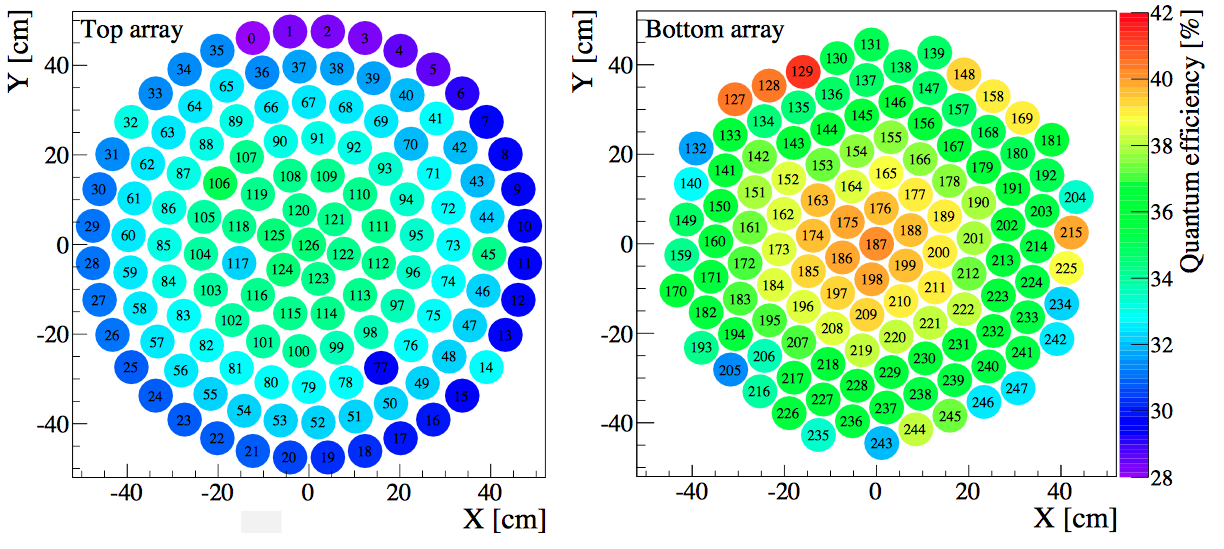
\includegraphics[width=\textwidth]{PMTQuantumEfficiency}
\caption{Quantum efficiency of top (left) and bottom (right) PMT arrays.  PMTs with highest QE are placed in the center of the bottom
array to maximize light collection while those with the lowest are placed in the outer region of the top.  Image credit:
\citeref{Aprile2017b}.}
\label{fig:xenon1t_pmt_qe}
\end{figure}

The two PMT arrays are supported by oxygen-free high thermal conductivity (OFHC) copper, with holes in which the PMTs are placed.  The
copper is then covered with polytetrafluoroethylene (PTFE) on the TPC-facing sides.  Screening meshes are situated between the bottom
array and cathode as well as the anode and top array.  Each can be biased to minimize electrical interference between the
phototubes and the drift and extraction fields.  While \citeref{Baudis2013} showed normal operation of R11410 PMTs at
$\geq 11\ \mathrm{kV\ cm^{-1}}$ the expected voltage for the cathode was $10 \mdash 100\ \mathrm{kV\ cm^{-1}}$ and decreasing the stress
on the phototubes is likely to be beneficial longterm.  The finished arrays are shown in \figref{fig:xenon1t_pmt_array}.

\begin{figure}
    \centering
    \begin{subfigure}[t]{0.5\textwidth}
        \centering
        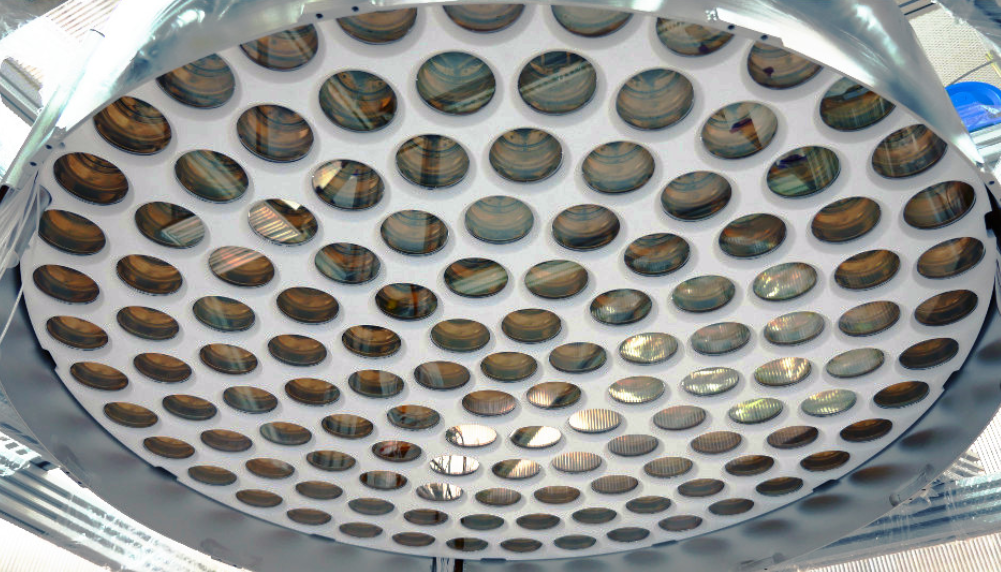
\includegraphics[height=4cm]{PMTTopArray}
    \end{subfigure}%
    \begin{subfigure}[t]{0.5\textwidth}
        \centering
        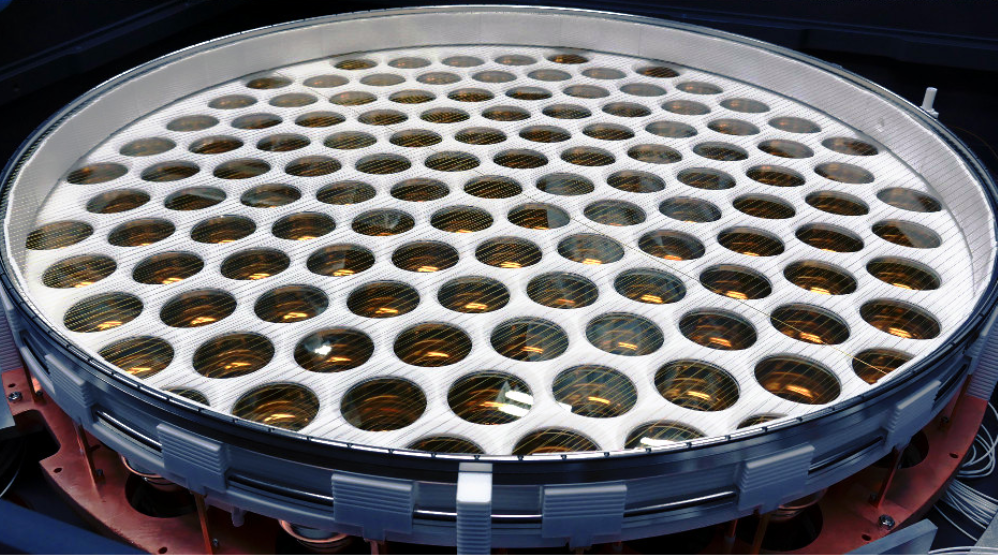
\includegraphics[height=4cm]{PMTBottomArray}
    \end{subfigure}
    \caption{XENON1T top (left) and bottom (right) PMT arrays.  Top PMTs are installed inside the diving bell in a radial distribution
    to minimize uncertainty in radial position reconstruction.  Bottom PMTs are installed below the cathode and screening mesh that
    limits interference between the PMT and cathode electric fields, both of which can be seen.  They are packed tightly
    together to maximize light collection.  Image credit: \citeref{Aprile2017b}.}
	\label{fig:xenon1t_pmt_array}
\end{figure}

\begin{figure}
\centering
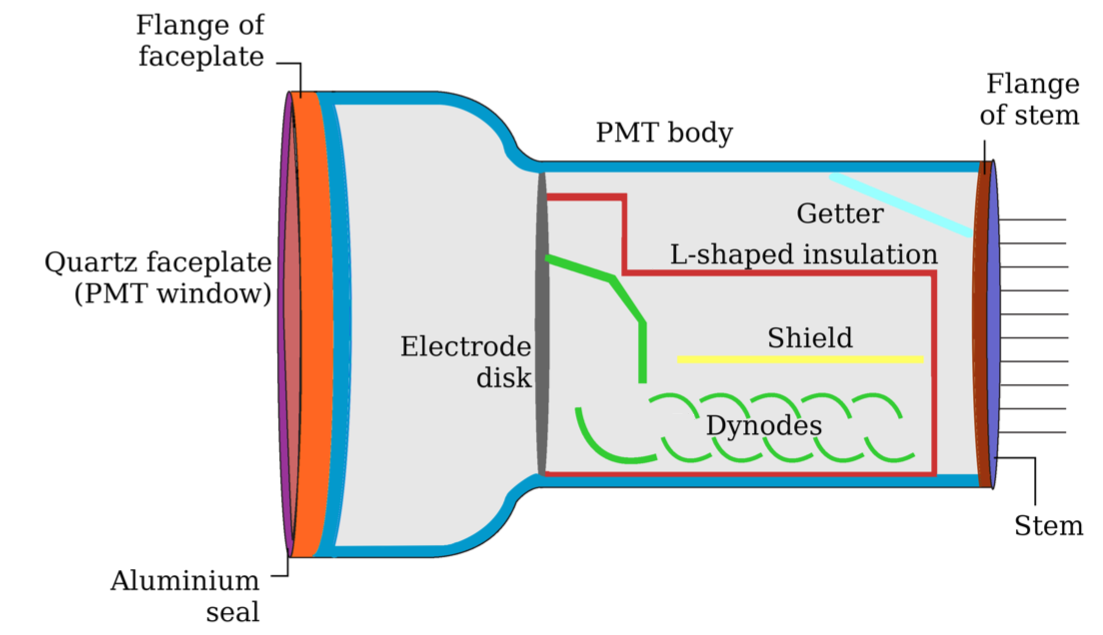
\includegraphics[width=0.8\textwidth]{PMTSchematic}
\caption{Schematic of the R11410-21 PMT.}
\label{fig:xenon1t_hamamatsu_pmt}
\end{figure}

The R11410-21 has 12 dynodes following the focusing electrode disk.  The first dynode is the largest and extends to the electrode to
maximize the probability of capturing photoelectrons.  A schematic can be be seen in \figref{fig:xenon1t_hamamatsu_pmt}.  The electrode,
dynode, and shield are stainless steel and are insulated with L-shaped quartz plates.  The window is
also made of quartz, since it is transparent to vacuum ultraviolet (VUV) photons.  Deposited on it is a low-temperature bialkali
photocathode.  The window is fixed with an aluminum seal to the faceplate flange, which along with the stem flange is constructed from
Kovar.  Because of the PMT body's large mass (71\% of total Kovar, 35\% of total) a low-\ce{^{60}Co} Kovar is chosen.  Finally, to insulate
the connections to each dynode the stem is ceramic.

Because radioactivity limits the fiducial volume and increases the event rate, making accidental coincidence and outlier events more
likely, XENON and Hamamatsu worked together to develop a highly radio-pure PMT.  There were several iterations of the R11410 model before
the R11410-21 was determined to be adequate.  Nearly all the \ce{^{137}Cs} and \ce{^{60}Co} comes from the Kovar, though the \ce{^{137}Cs}
content is negligible and the \ce{^{60}Co} is 3-10 times lower than older models.  The remaining screened isotopes, \ce{^{238}U},
\ce{^{228}Th}, \ce{^{228}Ra}, \ce{^{226}Ra}, and \ce{^{40}K}, are dominated by the ceramic stem (\citeref{Aprile2015}).  Unfortunately a
material that is more radio-pure and can insulate the dynode connections has not been found.  Sapphire was used in an iteration but
ultimately showed any improvement was minimal.

The dark count rate, or the number of signals per second above a threshold without a light source, is an important property to
characterize.  At ambient temperatures the primary cause is thermal electrons that scale with PMT voltage.  This becomes subdominant at
cryogenic temperatures to electron field emission and radioactivity (internal and external) as well as cosmic rays.  In a detector such
as XENON1T higher dark count rates make accidental coincidence more likely, which produces fake additional background and in the worst case
can place fake events in the signal region.  Because the rate is dependent on the threshold it can effectively be tuned.  However, because
for DM search we would like as low of a threshold as possible, choosing PMTs with low dark count rate is essential.

Another problematic feature is light emission from the phototube itself, where light is created inside the PMT and escapes through the
window.  It has been observed to mainly occur in one of two ways.  The first is through a discharge of intense light that can last for
several seconds.  This so-called ``flash" is bright enough to be easily observable to itself and by PMTs that are facing its
window.  However, the intensity can be so strong that it can take anywhere from several minutes to several hours for them to
recover.  Because they seem to occur spontaneously and are not well understood it is impossible to predict when a flash will occur.

The second variety is a subtle but often continuous stream of light.  Known as ``micro light emission" it is considerably harder to
identify.  Doing so requires facing two phototubes towards one another and measuring the dark rate of each one with and without the other
on.  The level of emission increases with temperature and bias voltage.  Keeping the PMTs at cryogenic temperatures during DM runs reduces
such effects, and voltages can be lowered to help further.  Still, if micro light emission continues the PMT cannot be used as it risks
contaminating the detected light from the true event population.

Directly following the pulse of a PMT hit a secondary pulse may occur.  Known as afterpulses, they can occur within 10s of
nanoseconds.  This can make them difficult to resolve from true pulses - especially S2s - that can have widths of several
microseconds.  However, they are an inevitable side effect when using PMTs so characterizing them properly is important.  There are three
mechanisms known to cause afterpulses.

The first is elastic scattering of the photoelectron with the first dynode, freeing \electron that shortly return to the dynode.  This
prompts afterpulses in the range of a few to tens of nanoseconds.  A second kind is thought to stem
from dark noise and single electrons but is not well understood.  It has a relatively uniform distribution in delay time up to several
microseconds.  Both of these afterpulses have relatively small areas of $\lesssim 2\ \mathrm{PE}$.

A photoelectron may occasionally ionize residual gas inside the PMT along its trajectory to the first dynode.  The molecule then drifts
towards the photocathode, expelling additional electrons.  The number of newly ejected electrons (area of afterpulse) depends
on the ion and the position of ionization.  The responsible ion can be determined by calculating the time between the true pulse and
afterpulse.  For R11410-21 this gives

\begin{equation}
\delta t_{\mathrm{ap}} = \frac{\pi}{4} \sqrt{\frac{2 m}{q V_{0}}} L
\end{equation}

where $\delta t_{\mathrm{ap}}$ is the delay time, $m$ and $q$ are the ion's mass and charge, and $V_{0}$ and $L$ are the potential
difference and length between the photocathode and first dynode (see \citeref{Barrow2017} for details).  Note that $\delta t_{\mathrm{ap}}$
does not depend on where the ionization occurred.  Thus, if we know the time between the true and afterpulse the ion - or more specifically
charge to mass ratio - can be calculated.  Pulse time differences range from several hundred nanoseconds to several microseconds.  These
correspond to the ``lines" in \figref{fig:xenon1t_pmts_ap} that extend to larger afterpulses.  The short timescales of S1s make them
unlikely to be grouped with an afterpulse, though for S2s this is more likely.

\begin{figure}
\centering
\includegraphics[width=\textwidth]{afterpulse_spectrum_pmt_21}
\caption{Afterpulses for one of the PMTs from XENON1T.}
\label{fig:xenon1t_pmts_ap}
\end{figure}

Because it is not possible to remove all residual gas any PMT will suffer from some ionization-based afterpulsing.  A better vacuum
corresponds to fewer afterpulses and a healthier PMT in general.  If the concentration of gas in the PMT vacuum were to increase it would
escalate the afterpulse rate.  Therefore if when using in xenon the Xe peaks grow over time the PMT most likely has a leak and should
be removed, as continued worsening of the vacuum will lead to deterioration and inability to operate the PMT.  All PMTs were tested before
being installed in XENON1T.  73 were rejected and replaced: 12 due to high dark count rates, 53 for light emission, and 8 for
afterpulsing.

The transit time (TT) is the time between the freed photoelectron and the arrival of the electron avalanche at the anode.  Variations in
the photoelectron's initial position as well as emitted velocity and angle cause deviations in the TT, which is characterized by the
transit time spread (TTS).  Because an event is observed by many PMTs the TTS quantifies how close together there signals should be.  Thus
smaller TTSs lead to a smaller integration window, decreasing accidental coincidence.  The TTS for all R11410-21 PMTs was measured, giving
a mean of $9.1 \pm 1.3\ \mathrm{ns}$ - a fraction of an S1.

It was shown by \citeref{Faham2015} that the probability of double photoelectron emission (DPE) in a number of PMTs, including the
R11410, is generally in the range of 0.18-0.24 - much higher than previously thought.  For The R11410 in particular they found the
probability to be $p_{\mathrm{dpe}} = 0.225 \pm 0.01$.  Any $p_{\mathrm{dpe}} > 0$ has some effect on a number of elements in a DM
search - however, with such a large value these cannot be ignored.  First it may be useful to define a second quantity closely
related to but not the same as the QE.  Following \citeref{Faham2015} the QE will be denoted as $\eta_{\mathrm{\mu}}$ and the fraction of
incident photons that produce one or more photoelectrons denoted $\eta_{\mathrm{p}}$.  Then they are related to one another by

\begin{equation}
\eta_{\mathrm{\mu}} = (1 + p_{\mathrm{dpe}}) \eta_{\mathrm{p}}
\label{eq:xenon1t_pmts_dpe}
\end{equation}

\noindent and we see that the measured QE alone will be misleading.  For one, it is common to require a PMT coincidence for an event to
be considered good - that is, $n$ PMTs must see a signal within a predetermined time window.  Using $\eta_{\mathrm{\mu}}$ will
\textit{overestimate} the likelihood of this happening, and $\eta_{\mathrm{p}}$ should instead be used.  Additionally, when the PMT
response is easily over threshold DPEs lead to incorrect resolution and yields unless accounted for.  In
\secref{subsubsec:er_nr_calibrations_parameter_determ_det_phys} during the electronic and recoil band fitting details on how to
appropriately account for all of these effects are shown.

An additional six Hamamatsu R8520 PMTs reside in LXe outside the TPC near the top electrode for studying calibrations.  These PMTs have
been used in a number of LXe TPCs including XENON100, the predecessor to XENON1T (\citeref{Goetzke2017}, see \citeref{Aprile2012a} for
details on XENON100).




\subsection{TPC}
\label{subsec:xenon1t_tpc}
The XENON1T time projection chamber is cylindrical with a 96.9 cm height and 47.9 cm diamater.  It encloses a target mass of 2.0 tons where
light and charge can be measured.  A schematic is shown in \figref{fig:xenon1t_tpc_tpc}.  The interior of the vertical wall consists of 24
PTFE panels that were treated with diamond tools to
maximize VUV reflectivity.  Each interlocks with adjacent panels to achieve light-tightness, and the system is designed so that despite
the high thermal expansion coefficient the radius does not contract when lowered to $-96^{\circ}\ \mathrm{C}$.  Outside the PTFE are 74
field shaping rings made of low-radioactivity OFHC copper, each with a cross section of ${\sim} 10 \times 5\ \mathrm{mm^{2}}$.  They are
supported by 18 PTFE pillars stationed around the circumference.  Two redundant
chains connect adjoining rings via $5\ \mathrm{G \Omega}$ resistors, each with a $25\ \mathrm{G \Omega}$ resistor between the bottom and
cathode.

\begin{figure}
\centering
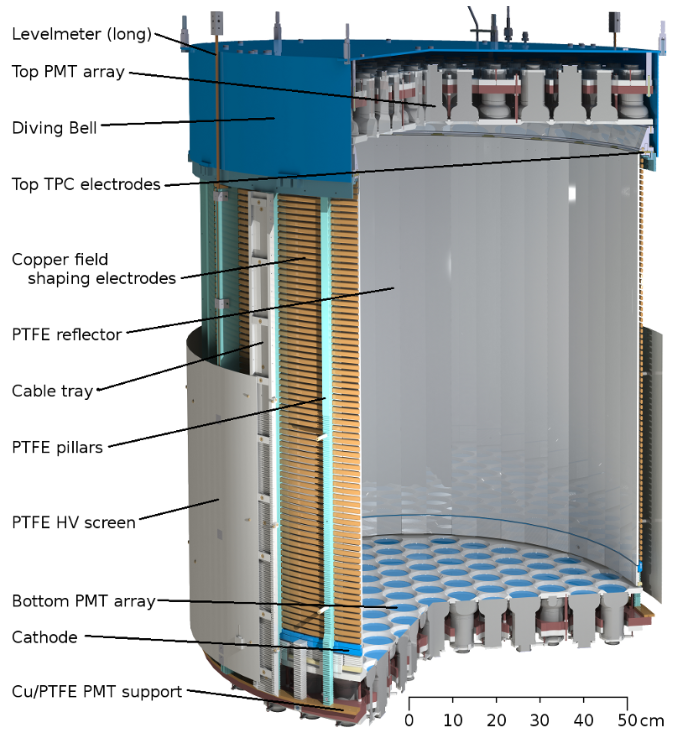
\includegraphics[width=0.8\textwidth]{XENON1TTPC}
\label{fig:xenon1t_tpc_tpc}
\end{figure}

There are five TPC electrodes that control the electric fields: the cathode, gate, anode, and top and bottom screening meshes.  They have
wired diameters of $\mathcal{O}(100)\ \mathrm{\mu m}$ and were designed to maximize S1 light collection.  The cathode is connected to a
PNC150000-1 NEG high voltage supply and pre-filling tests successfully reached voltages beyond -100 kV.  48
cm below the cathode is the bottom screening mesh (mentioned in \secref{subsec:xenon1t_pmts}).  The mesh is 12 mm above the bottom PMT
array and can be biased to reduce unwanted effects from the PMT and cathode E-fields.  The cathode and bottom screening mesh consist of
parallel wires and are gold-plated stainless steel, the latter of which increases the workfunction.  The gate rests just below the
liquid-gas interface and defines $z = 0$.  The anode is
situated 5 mm above the gate and is connected to a CAEN A1526P unit.  The fifth and final electrode is the top screening mesh 58 mm above
the anode and 11 mm below the top PMT array, and serves the same function is the same as the bottom mesh.  The top three electrodes are
made of stainless steel and are hex-etched.  Details for each electrode can be seen in \tabref{tab:xenon1t_tpc_electrodes} and
\figref{fig:xenon1t_tpc_efield} shows the simulated electric field for the settings during the first science run, Science Run 0.

\bgroup
\def\arraystretch{1.2}
\begin{table}
\centering
\resizebox{\textwidth}{!}{
\begin{tabular}{cccccc}
\hline
Electrode & Type & Diamater & Material & Transparency & Position \\
\hline
Top screening & hex meshed & $178\ \mathrm{\mu m}$ & stainless steel & 96.5\% & 63 mm \\
Anode & hex meshed & $178\ \mathrm{\mu m}$ & stainless steel & 89.8\% & 5 mm \\
Gate & hex meshed & $127\ \mathrm{\mu m}$ & stainless steel & 92.7\% & 0 mm \\
Cathode & parallel wires & $216\ \mathrm{\mu m}$ & gold-plated stainless steel & 97.2\% & -969 mm \\
Bottom screening & parallel wires & $216\ \mathrm{\mu m}$ & gold-plated stainless steel & 97.2\% & -1017 mm \\
\hline
\end{tabular}
}
\caption{Properties for TPC electrodes.  The cathode and bottom screening mesh have high transparency to optimize S1 light collection and
are gold-plated to increase workfunction.}
\label{tab:xenon1t_tpc_electrodes}
\end{table}

\egroup

\begin{figure}
\centering
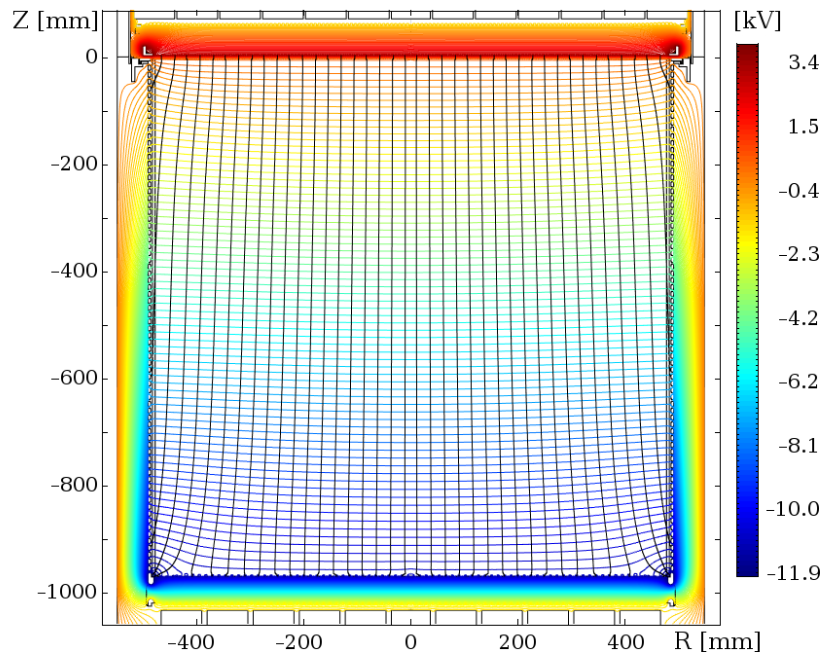
\includegraphics[width=0.8\textwidth]{ElectricField}
\caption{Finite element (COMSOL Multiphysics) simulation for E-field inside and around the TPC.  Field and equipotential lines are
shown.  The voltages for the cathode, gate, and anode are -12, 0, and 4 keV, respectively, or the settings for Science Run 0.  The field
is mostly uniform throughout the detector, minimizing possible biases that come from recombination, impurity attachment, etc.  Image
credit: \citeref{Aprile2017b}.}
\label{fig:xenon1t_tpc_efield}
\end{figure}

Four parallel-plate capacitors measure the liquid level.  They have a range of 10 mm with $30\ \mathrm{\mu s}$ precision and can be used
for observing tilts or raising (lowering) the TPC.  The liquid level's height is adjustable a gas-exhaust tube, and maintained with a
so-called ``diving bell" that uses controlled gas flow from purification to pressurize the GXe inside the TPC.  Two cylindrical levelmeters
with a range of 1360 mm extend from the bottom PMT array to above the diving bell and are used for filling and recovery.  Placed around the
field cage are cable trays that power and transfer signal from the PMTs.  They are made of PTFE and the cables are held
in place by PTFE spacers (\textbf{check if spacers is right word}).



\subsection{Cryogenics}
\label{subsec:xenon1t_cryo}
The TPC is stationed in the center of the water Cherenkov detector (\secref{subsec:xenon1t_water_shield}) and is encompassed by the inner
cryostat.  The cryostat
is stainless steel and electropolished to reduce radon emanation (\secref{subsubsec:backgrounds_electronic_radon}), since it is in direct
contact with the xenon.  It is 1960 mm tall by 1100 mm diamater and is metal-sealed
with Helicoflex.  Surrounding it is the 2490 mm tall by 1620 mm diamater outer cryostat.  It is also composed of stainless steel but
because there is no contact with xenon electropolishing is unncessary.  Materials were screened prior to construction for low-radioactivity
selection.  The two are thermally isolated by Torlon polyamide-imide spacers and
vacuum between them.  Heat loss is further mitigated to ${\sim} 75\ \mathrm{W}$ by aluminized mylar foil wrapped around the inner vessel.

A 10 m high stainless steel support structure was built inside the water tank.  Attached are three M20 rods that suspend the
cryostat.  They can be adjusted independently to tilt the cryostat, thereby changing the inclination of the LXe level with respect to the
TPC.  A chain secures the bottom of the outer vessel to the water tank floor to counteract buoyancy forces when the cryostat is empty.  A
double-walled pipe with inner and outer diameters 254 and 406 mm, respectively, connects with purification (\secref{subsec:xenon1t_pur}),
cooling,
pressurization for diving bell, and emergency recovery, and carries the PMT and auxiliary cables.  The voltage for the cathode is guided
in a separate pipe.  A schematic of the cryostat is shown

\begin{figure}
\centering
\includegraphics[width=0.8\textwidth]{CryostDiagram}
\caption{Diagram of the cryostat.  Image credit: \citeref{Aprile2017c}.}
\label{fig:xenon1t_cryo_cryostat_diagram}
\end{figure}

A total of 3.5 tons of xenon is stored in the cryostat.  In addition to the 2.0 inside the TPC, the extra 1.5 is LXe between the
TPC and inner vessel or GXe above the liquid level.  The nominal LXe temperature is $T_{0} = -96^{\circ}\ \mathrm{C}$.  Gas near the top of
the cryostat is liquified by pulse-tube refrigerators (PTRs) into a funnel and flows back to the TPC through a designated pipe and
deposited in the inner vessel beneath the TPC.  Because
the PTRs are higher than the TPC the flow is guided by gravity.  \figref{fig:xenon1t_cryogenics_schematic} shows the layout of the
cryogenic
system.  The two PTRs occupy independent cooling towers and can each deliver ${\sim} 250\ \mathrm{W}$ of cooling power, and with
a total heat xenon heat load of ${\sim} 150\ \mathrm{W}$ only one needs to be active at any time.  The cooling towers along with much of
the
GXe are located in the service building outside of the water tank  Each PTR connects to a copper cold finger
inside the inner cryostat so they can be removed without exposing the xenon to air.  A proportional-integral-derivative (PID) controller
monitors and adjusts the temperature of a resistive heater on the coldfinger to maintain stable pressure and temperature.

A third cooling tower uses liquid nitrogen ($\mathrm{LN_2}$) and is used in the case of an emergency if both PTRs are being serviced or the
heat load becomes too great from e.g. loss of power or insulation vacuum.  The $\mathrm{LN_2}$ flows from the $10 \mathrm{m^3}$ tank that
is used by ReStoX (\secref{subsec:xenon1t_restox}).  The cooling power can regulated by adjusting the $\mathrm{LN_2}$ evaporation rate.  In the event the PTRs
lose power the $\mathrm{LN_2}$ cooling tower must react immediately to prevent rising pressure that can be damaging to PMTs among other
things.  Sensors and controllers monitoring such a power loss are powered with uninterruptible power supplies (UPSs) to ensure a successful
transition and operation of $\mathrm{LN_2}$.

\begin{figure}
\centering
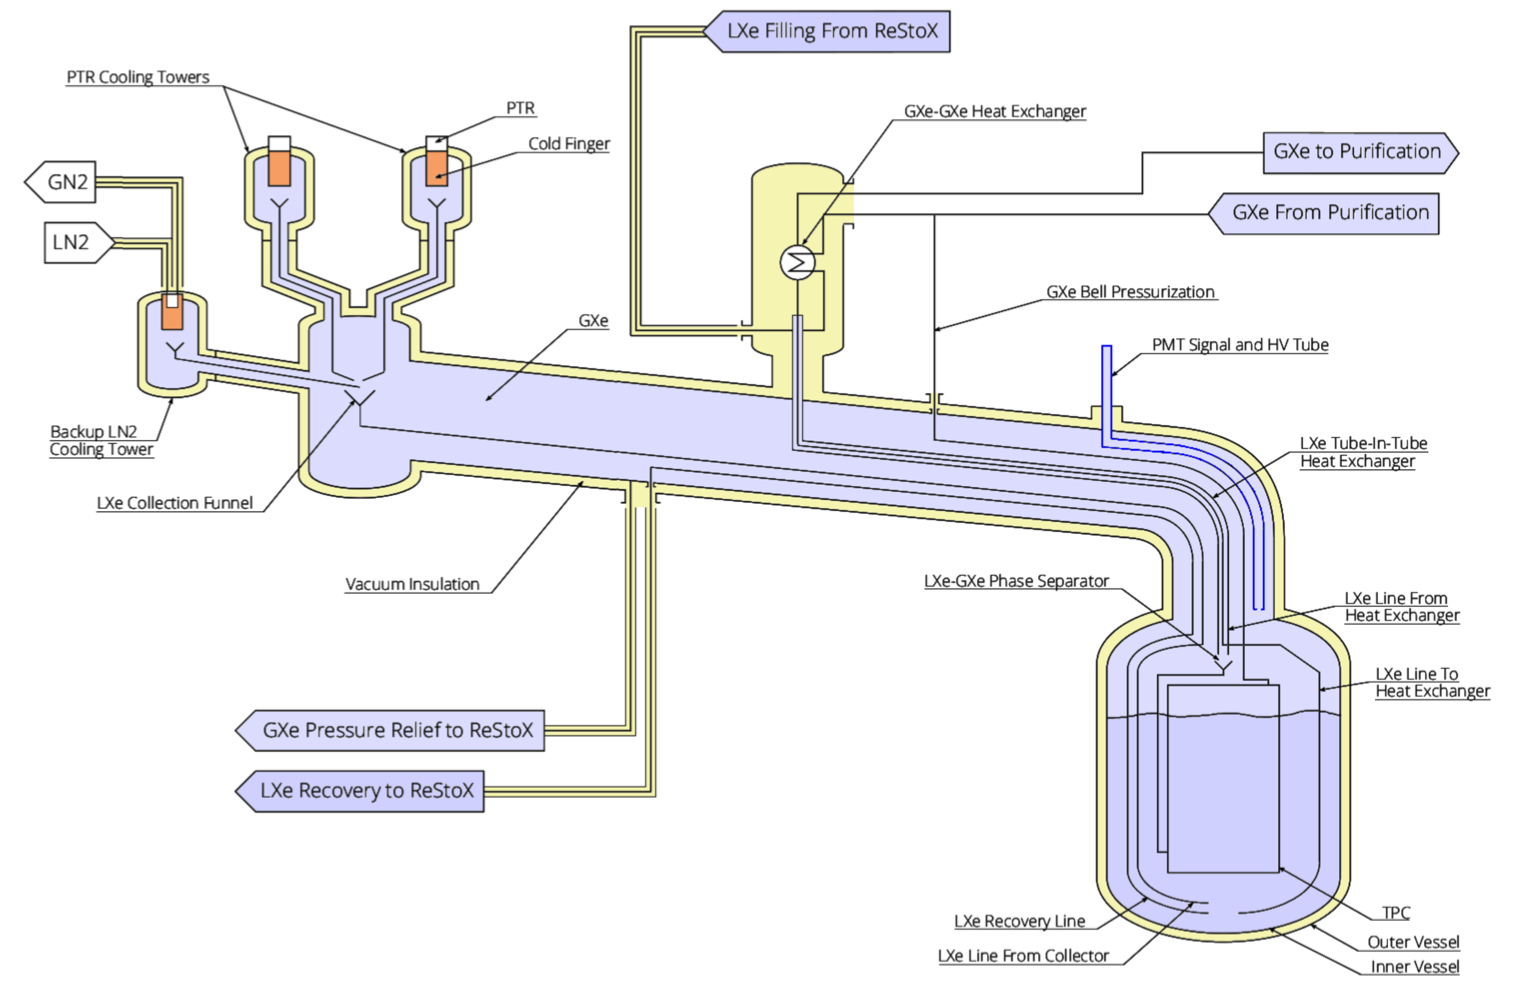
\includegraphics[width=\textwidth]{CryostatSchematic}
\caption{Layout of the cryogenic system.  Three cooling towers - two with PTRs and one backup $\mathrm{LN_2}$ - liquify GXe to return to
the TPC.  LXe is carried from the bottom of the cryostat to the purification system (\secref{subsec:xenon1t_pur}) through a heat
exchanger system, where
returning xenon is inserted into the bottom of the TPC with excess gas diffusing into the GXe.  A fraction of purified GXe is extracted
before the heat exchanger and used to maintain pressure inside the diving bell.  ReStoX (\secref{subsec:xenon1t_restox}) connections are
also shown.  Image credit: \citeref{Aprile2017b}.}
\label{fig:xenon1t_cryogenics_schematic}
\end{figure}

Connections to purification and ReStoX are shown in \figref{fig:xenon1t_cryogenics_schematic}.  The LXe carried to the purification system
passes through a heat exchanger system discussed in \secref{subsec:xenon1t_pur}.  This is not the case for recuperation since the xenon
does not need to be gaseous.

LXe from the beneath the TPC (near liquid line from PTRs) is removed for purification.  Once the xenon removed from the LXe it passes
through a two-phase heat exchanger system.  The function of the heat exchanger is for GXe (returning to the TPC) and LXe (leaving) to
exchange thermal energy.  This way the returning xenon is cooled before it reaches the TPC, and likewise removed xenon is heated before
the purification.  The first step of the system is the ``tube-in-tube" component where two concentric tubes carrying LXe (GXe) away from
(towards)
the TPC.  The second component is a plate heat exchanger and is closer to the purification system (i.e. returning xenon passes through
before tube-in-tube).

We can define the heat exchange
efficiency $\epsilon$ as the fraction of heat necessary for temperature change and vaporization that stays outside of the system.  A higher
efficiency results in greater thermal energy transferred between the GXe and LXe and thus decreases the heat load on the system.  This is
because instead of GXe entering the cryostat at roughly
room temperature, it returns at approximately that of LXe, with much of it having condensed to LXe, putting less stress on the
PTRs.  An essential ingredient of the heat transfer is the latent heat, which comprises ${\sim} 80\%$ of the total exchange.  The
difference in vaporization temperature of the outgoing xenon and condensation temperature of incoming xenon is given by

\begin{equation}
\Delta T_{\mathrm{ph}} = T_{\mathrm{gl}} (P_i) - T_{\mathrm{gl}} (P_o)
\label{eq:xenon1t_cryo_latent}
\end{equation}

where $T_{\mathrm{gl}} (P)$ is the temperature of the gas-liquid phase transition that depends on pressure, and $P_i$ and $P_o$ are the
pressures of the incoming and outgoing xenon, respectively.  Because the conditions of the dynamical gas flow
(\secref{subsec:xenon1t_pur}) cause $P_i > P_o$, $\Delta T_{\mathrm{ph}} > 0$, making it effective at heat transfer
(\citeref{Aprile2012b}).  A study with the Demonstrator - the
experiment used to for research and development for XENON1T - showed a heat exchange efficiency of
two heat exchangers in series of $\geq 96\%$ (\citeref{Aprile2012b}).  Following the parallel-plate exchanger a heater provides additional
thermal energy to the xenon moving towards the purification system.  The different systems that handle the xenon can be seen in
\figref{fig:xenon1t_cryo_overview}.

\begin{figure}
\centering
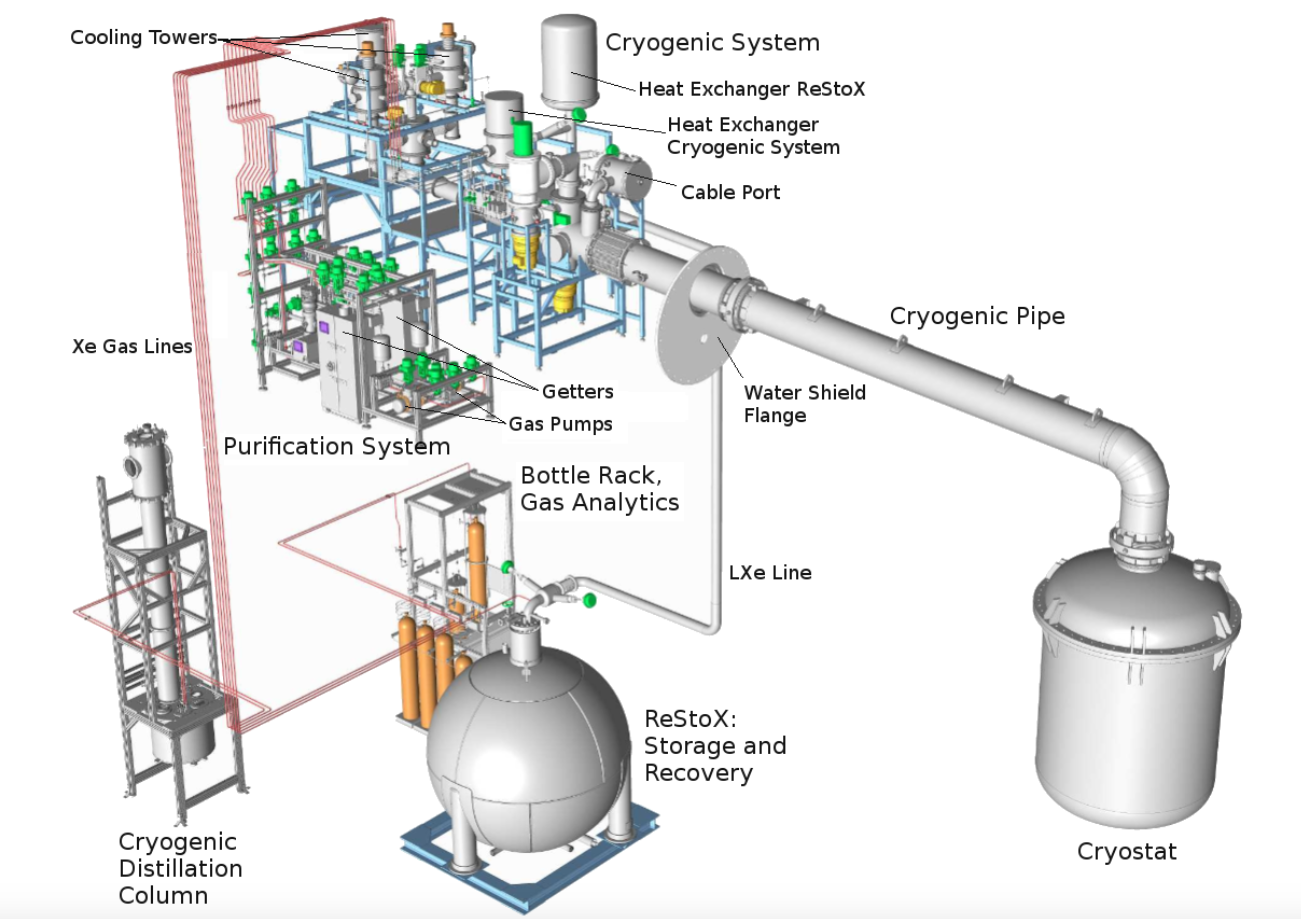
\includegraphics[width=\textwidth]{CryoOverview}
\caption{The various systems that handle xenon in the experiment: cryostat, cryogenics, purification, cryogenic distillation column,
ReStoX, bottle racks, and gas analytics station.  The water shield flange defines the region between the service building and the water
Cherenkov detector.  Image credit: \citeref{Aprile2017b}.}
\label{fig:xenon1t_cryo_overview}
\end{figure}



\subsection{Purification}
\label{subsec:xenon1t_pur}
Contamination in LXe can present a number of problems.  As mentioned in \secref{subsec:tpcs_working_principle} electronegative
impurities (e.g. O$_2$, H$_2$O, N$_2$O, etc.) will attach to drifting $e^-$, reducing the number that reach
the liquid surface and thus the S2.

Impurities will also attenuate scintillation, which pushes our energy threshold up as fainter signals become harder to detect.  This is
described by

\begin{equation}
I(x) = I_0 e^{-x / \lambda_{\mathrm{att}}}
\label{eq:xenon1t_pur_atten}
\end{equation}

where $I_0$ is initial number of photons, $I(x)$ is the number after traveling a distance $x$, and $\lambda_{\mathrm{att}}$ is the
attenuation length.  $\lambda_{\mathrm{att}}$ is dependent on the absorption and scatter lengths, $\lambda_{\mathrm{abs}}$ and
$\lambda_{\mathrm{scat}}$.  The absorption length describes the true loss of photons while the scatter refers to photons that elastically
scatter without energy loss.  The attenuation length can then be written
$1 / \lambda_{\mathrm{att}} = 1 / \lambda_{\mathrm{abs}} + 1 / \lambda_{\mathrm{scat}}$.  \figref{fig:xenon1t_pur_absorption_spectra} shows
the Xe scintillation spectrum along with the absorption coefficients for \otwo and \htwoo vapor at concentrations of 1 ppm.  We can see
there is large overlap at lower wavelengths - especially for H$_2$O - and that observations under these circumstances would lead to an
incorrect measurement of the scintillation spectrum.  In addition to electronegative there are intrinsic
impurities including Kr and Rn but these are discussed in \secref{subsec:xenon1t_kr_dist}.

Electronegative impurities come primarily from outgassing of detector materials.  They have different \electron attachment rates (see
\figref{fig:attachment_rate} for examples) so are measured in O$_2$-equivalent - that is, the analogous concentration of oxygen if it
were the only contaminant.  For LXe experiments the necessary concentration is $\mathcal{O}(10^{-9})$ parts per billion (ppb) or less.

In addition
to the GXe from the TPC (after passing through heat exchanger and heater as described in \secref{subsec:xenon1t_cryo}), connections are
made between
each of the cooling towers and the purification system.  Because impurities are lighter than xenon we can anticipate them having a larger
presence in the gas.  While the GXe impurity concentration has no direct effect on \electron loss, impurities should migrate between the
LXe and GXe.  Purifying the GXe then should largely reduce the impurities that pass into the liquid.

Xenon from ReStoX  (\secref{subsec:xenon1t_restox}) and bottles are also connected to the purification system.  A separate heat exchanger
sits between ReStoX and purification but is less effective when xenon is not incoming and outgoing (not during detector filling).  In
addition to cleaning the Xe as it is transfered to the from RestoX to the cryostat, the purification system connects ReStoX to the Kr
distillation column (\secref{subsec:xenon1t_kr_dist}).  The column returns the xenon after distillation to purification.  All systems that
feed into the purification system do so before the getters and are available as outputs as well.  A small tube between the purification
and cryostat before the heat exchanger siphons GXe to the TPC bell to maintain pressure, and is regulated by a flow controller.  The
numerous connections makes the purification system a hub for transferring xenon between systems.

\begin{figure}
\centering
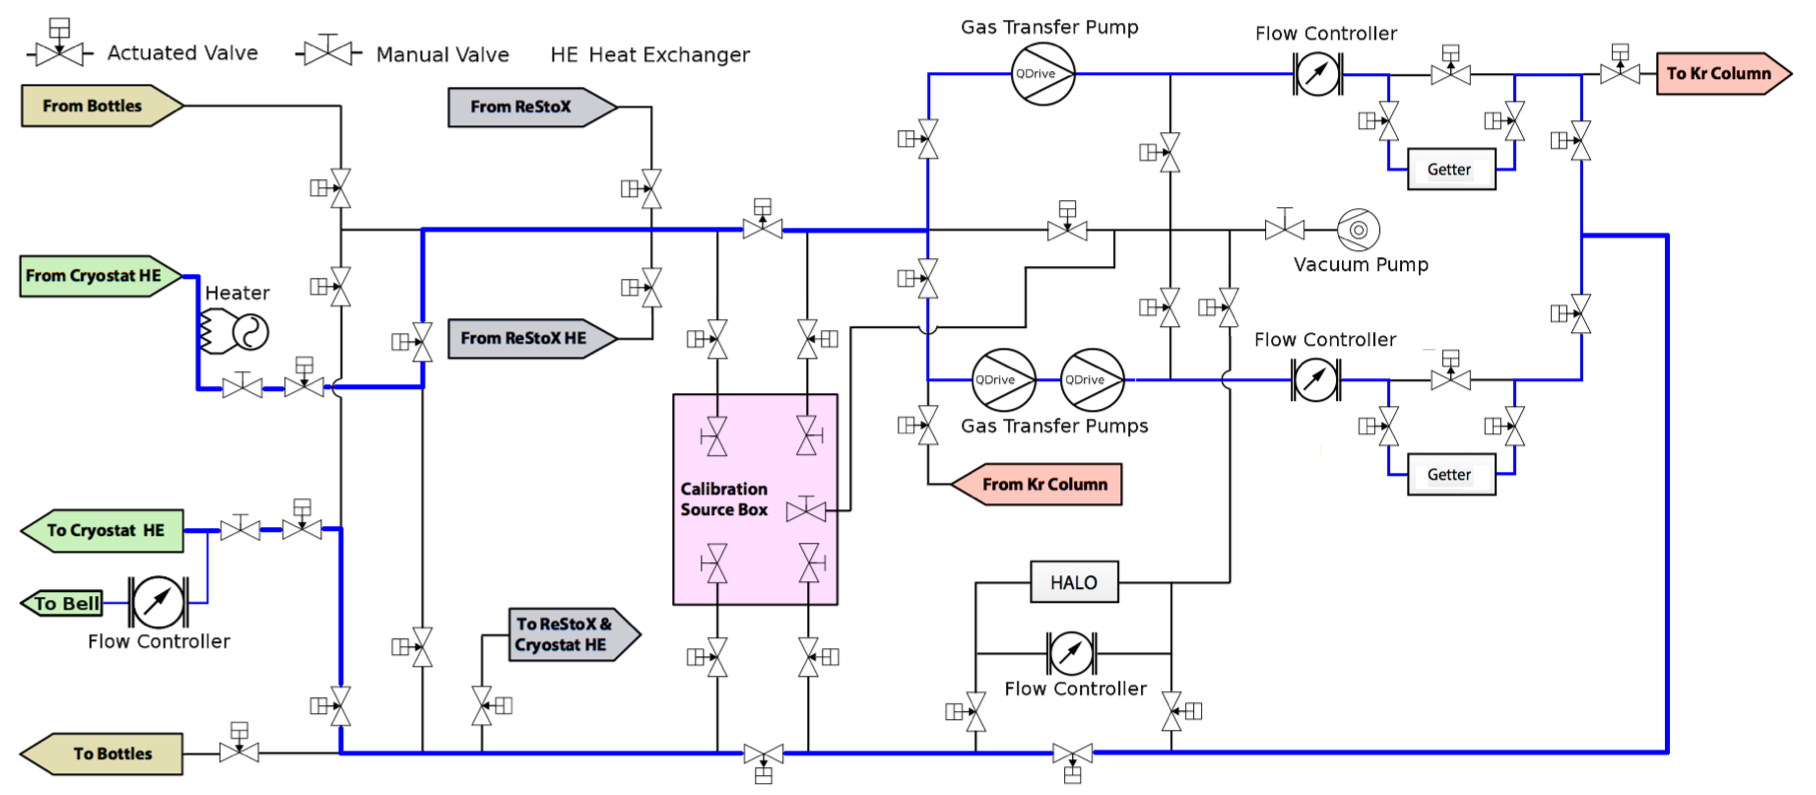
\includegraphics[width=\textwidth]{PurificationLayout}
\caption{Layout of the purification system.  The standard flow path during normal operations is highlighted in blue.  Image credit:
\citeref{Aprile2017b}.}
\label{fig:xenon1t_pur_schematic}
\end{figure}

The purification system consists of two redundant purification loops, each of which can operate independently of the other.  The flow
is driven by CHART QDrives, with one on one loop and two on the other.  They were chosen for their high-capacity and hermetically sealed
pump volume, the latter of which was not true with KNF pumps that were used in XENON100 (\textbf{check this}).  This is important because
exposure to air could cause a significant drop in purity, and has occurred in the past with KNFs.  They are
magnetically-resonant and operate via a compression space with oscillating externally-driven pistons.  Motors, valves, and pistons are
not lubricated, making it an excellent choice for high-purity.  Unfortunately Q-Drives emanate \ce{^{222}Rn} can require frequent
maintenance if operated at too great a voltage (for larger flow).  For the former \ce{Rn} emanation measurements were made prior to
installation with the lowest being chosen.  For the latter they are operated at safe conditions and since the beginning of Science Run 0
no issues have arisen.  It turns out the limiting factor on our circulation speed is not a result of the pumps but the pressure difference
from tubes leading to the system caused by too small a radius.  With the upgrade to XENONnT these will be replaced with larger-radii.  One
Q-Drive is installed in one loop and two in the other.

\begin{figure}
\centering
\includegraphics[width=0.6\textwidth]{calibration_source_box}
\caption{Layout of the calibration source box in the purification system.  Locations of \ce{^{220}Rn}, $^{83\mathrm{m}}\mathrm{Kr}$, and
\ce{CH_3T} are encompassed by dotted rectangles.  Filters are installed to catch debris.  Connections to and from the cryostat (turquoise)
and pumps and getters (red) are shown.  The vacuum pump (yellow) is used to evacuate the chamber before use.}
\label{fig:xenon1t_pur_cal_box_schematic}
\end{figure}

The flow of the GXe is maintained by two MKA 1579A mass-flow controllers - one on either branch.  The assumption before the experiment went
online was these would limit the speed when necessary, but because we did not achieve our goal these have minimal impact.  Still, they can
be used for further restriction.  The xenon then passes through SAES PS4-MT50-R high-temperature rare-gas purifiers, or getters.  They
use heated ($400^{\circ}\ \mathrm{C}$) zirconium to form unbreakable bonds with carbide, nitride, and oxide, lowering the impurity content
to $< 1 \mathrm{ppb}$ (\citeref{Aprile2017b}).  A bypass valve allows the xenon to pass un-purified in the event that the it does not need
to be cleaned.

A Tiger Optics HALO+ H$_2$O monitor measures the water content in the purified GXe to track the purification efficiency.  It can measure
concentrations down to 400 ppt.  As with the getters, it can be bypassed.  The Xe is then forwarded to the cryostat, bell, ReStoX, or
bottles (Kr column occurs after the purification loops before the HALO).

The components of the system are electropolished and able to be baked up to ${\sim} 120^{\circ}\ \mathrm{C}$ for decreased outgassing during
operation.  The purification system has a number of valves that allow the versatility described in this section.  The majority are
pneumatic and can
be operated remotely with the slow control system (\secref{subsec:xenon1t_detector_slow_control}).  The remainder are manual valves
situated in select locations: to and from the cryostat,
inside the calibration box, and before the vacuum pump, which can be used to evacuate individual sections or all of the system.  These are
in place as a precaution against accidental openings of the actuated valves that could produce problems.


\subsection{ReStoX}
\label{subsec:xenon1t_restox}
The Recovery and Storage system for XENON1T (ReStoX) hosts xenon not in use by other systems.  It is located roughly 7 on the ground floor of the
service building.  With a volume of 4.95 m$^{3}$
(diameter of 2.1 m), wall thickness of 28 mm, and ability to withstand pressures up to 73 bar, it can support as much as 7.6 tons of xenon
as a gas, liquid, or super-critical fluid.  It is constructed from stainless steel and insulated with vacuum from an outer sphere, where
thermal conductance is minimized with superinsulation and limited contact to an external heat load of ${\sim}50\ \mathrm{W}$.  To limit
impurity contamination while the Xe is in ReStoX the vessel and valves are metal sealed and electropolished.

The xenon is cooled by LN$_2$ that is housed in a 10 m$^3$ dewar adjacent to the service building.  This is done in part with 16 LN$_2$
lines that are welded to the inner vessel's outer surface.  To prevent over-cooling 16 stainless steel fins inside increase heat
exchanging.  A condenser and heater in the middle are used when the xenon is stored as a liquid, which is the nominal state of
operations.  The heater ensures solid xenon does not block pipes so Xe can transfer freely with other systems.  The total cooling power is
spread over 4.3 m$^2$ of copper with magnitude of over $>3\ \mathrm{kW}$.

\begin{figure}
\centering
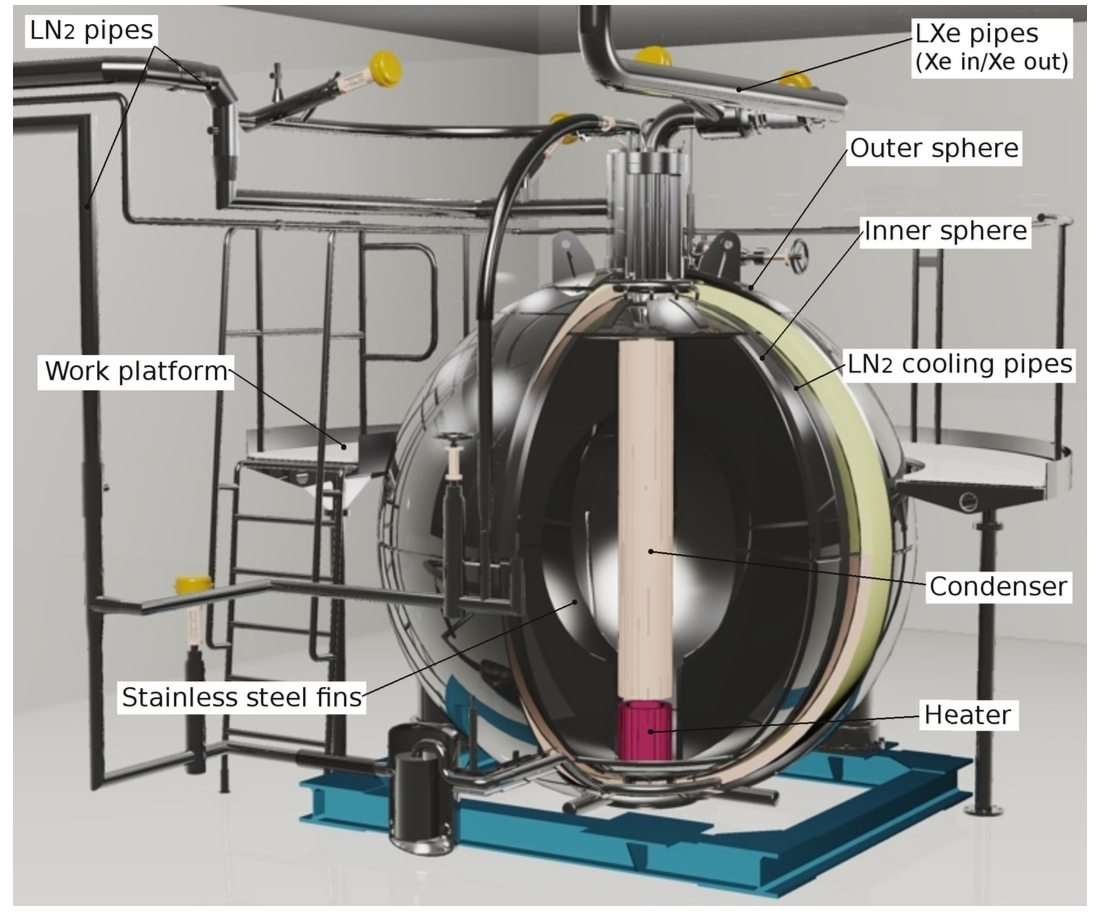
\includegraphics[width=0.8\textwidth]{ReStoX}
\caption{Image credit: \citeref{Aprile2017b}.}
\label{fig:xenon1t_restox_pic}
\end{figure}

Previous LXe experiments would fill the detectors by condensing the GXe from storage.  Similarly, recovery was done by allowing the LXe
in the cryostat to evaporate.  While this was achievable for detectors with $\mathcal{O}(100)\ \mathrm{kg}$ of xenon, doing so
(\textbf{maybe it is just for filling, check}) for XENON1T would require approximately two months, and fast recovery in the event of an
emergency would not be possible.  This is solved through the purification system, which as mentioned in \secref{subsec:xenon1t_pur} can
pump xenon between systems (\textbf{check with someone about how xenon is recovered}).



\subsection{Krypton Distillation}
\label{subsec:xenon1t_kr_dist}
Commercial high-purity xenon generally has \ce{Kr} concentrations from 1 ppm down to 10 ppb.  This is not clean enough for LXe dark matter
detectors so additional distillation is necessary.  The reason for restricting the
krypton content is \ce{^{85}Kr}, which undergoes \betadecay with an end-point energy of 687 keV and a half-life of 10.76 years.  With
an expected fraction $\mathrm{^{85}Kr / ^{nat}Kr = 2 \times 10^{-11}}$ the required \ce{^{nat}Kr}/Xe concentration for its background to be
less than radon is $< 200\ \mathrm{ppq}$.  Details of the \ce{^{85}Kr} background can be found in \secref{sec:backgrounds}.

To achieve the intended purity we use a Kr distillation column, seen in \figref{fig:xenon1t_kr_dist_column}.  The column is has a total
height of 5.5 m and is kept in an insulation vessel at $10^{-5}\ \mathrm{mbar}$ to minimize thermal losses (\citeref{Aprile2016b}).  GXe
that is passed to the column enters through a heat exchanger and is
liquified by the input condenser.  The input condenser uses a cryo-cooler (Leybold CP-50) at $-98^{\circ}\ \mathrm{C}$ and maximal power
of 100 W.  Next it passes to the package tube, built with 2.8 m of structured stainless steel package material (Sulzer EX) 45 cm in
diamater that has feeding ports for both liquid and gaseous xenon.  At the top of the tube is a second cryo-cooler (Leybold CP-140T)
operating at $-98^{\circ}\ \mathrm{C}$ with 200 W.  Liquified xenon will fall towards the bottom, where it is stored and heated by a
reboiler with a maximum of 300 W.  The Kr, with a lower atomic mass will drift towards the top of the column but will not liquify as its
boiling point is lower than $-98^{\circ}\ \mathrm{C}$.  Siphoning the xenon at the top then removes Kr at a much higher concentration than
present in the inlet GXe.  Purer Xe at the bottom is extracted where it passes through the heat exchanged before returning to the
purification system or ReStoX (\textbf{check this}).

\begin{figure}
\centering
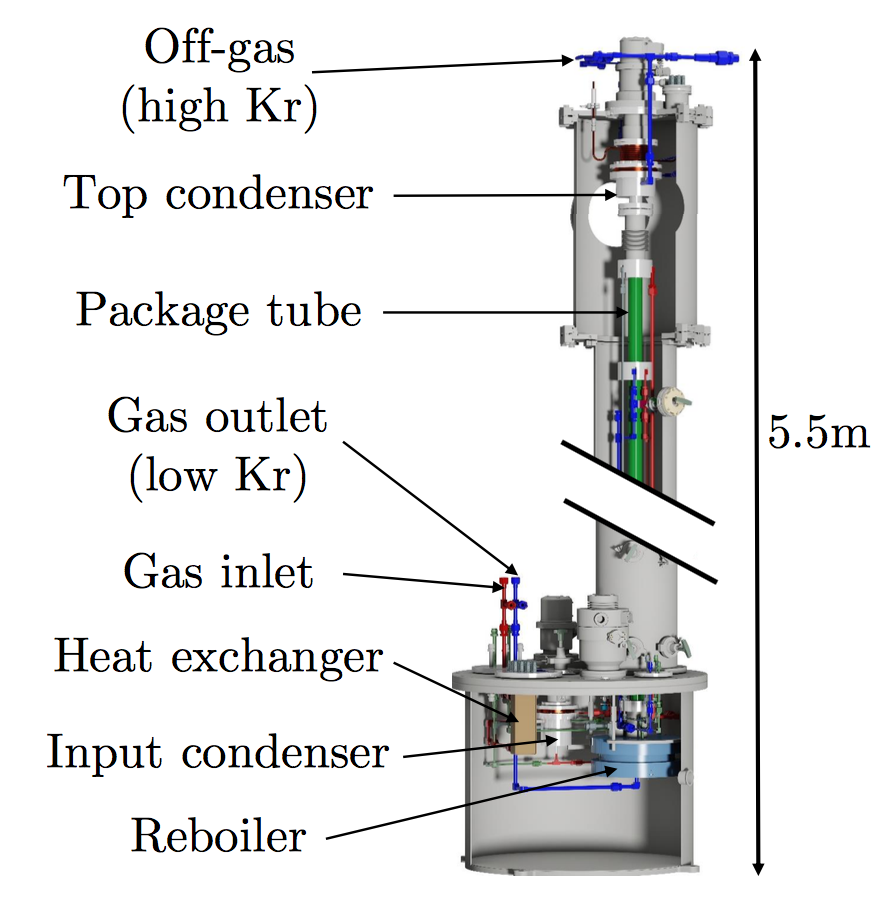
\includegraphics[width=0.6\textwidth]{KrColumn}
\caption{Image credit: \citeref{Aprile2017b}.}
\label{fig:xeno1t_kr_dist_column}
\end{figure}

After installed at LNGS the reduction of \ce{^{nat}Kr}/Xe was found to be $6.4_{-1.4}^{+1.9} \times 10^{5}$
(\citeref{Aprile2016b}).  Inlet flows have been shown to be stable up to 18 slpm, but running all ReStoX xenon through distillation before
cryostat filling would take ${\sim}3$ weeks.  For this reason an ``online" removal system was used, where the xenon was distilled during
science run data taking.  Over 70 days 7\% of xenon passing through purification was diverted to the column and a total 0.07\% was
removed.  An initial \ce{^{nat}Kr}/Xe concentration of 60 ppb was decreased to $360 \pm 60\ \mathrm{ppq}$, the lowest ever realized in a
LXe dark matter experiment.  Such low concentrations are measured by a rare gas mass spectrometer (RGMS) that uses cryogenic gas
chromotography to separate the Kr from Xe, followed by a mass spectrometer for Kr measurement (\citeref{Lindemann2014}).

A second low-energy background comes from the \ce{^{222}Rn} decay chain.  While the distillation column was built and intended for Kr,
it was shown to work in a single stage distillation (\citeref{Bruenner2017}) and subsequently XENON100
(\citeref{Aprile2017d}).  It operates using the reverse principle, i.e. Rn-enriched xenon is coalesces near the bottom of the column.



\subsection{Water Shield}
\label{subsec:xenon1t_water_shield}
Limiting radiation from outside the experiment is essential to a dark matter search.  An active water Cherenkov detector encompasses the
cryostat, spanning 9.6 m in diamater and 10.2 m high.  It is filled with deionized water, which can fill the detector at up to
$2.2\ \mathrm{m^{3}/hour}$.  The tank shields the cryostat from neutrons and \gammarays that originate underground (from e.g. rocks),
decreasing the event rate by orders of magnitude.  It can identify muons as well as muon-induced neutrons by detecting showers initiating
outside the water tank.  If an event in the TPC coincides with one in the water tank it will usually be excluded incase the two are
related, acting as a muon veto.  The flux of muons at LNGS is $3.31 \pm 0.03 \times 10^{-8}\ \mathrm{cm^2\ s^{-1}}$ with average energy
${\sim}270\ \mathrm{GeV}$ (\citeref{Aprile2017b}).

84 Hamamatsu R5912ASSY PMTs are placed in five rings along the inner wall of the tank, each 2.5 m apart in height.  The lowest
($z = 0\ \mathrm{m}$) and highest ($z = 10\ \mathrm{m}$) each contain 24, while the three between them have 12.  The quantum efficiency
is ${\sim}30\%$ between 300-600 nm.  To increase the chance of photon detection the inner wall is coated with foil (3M DF2000MA) that has
nearly 100\% reflectivity at $> 400\ \mathrm{nm}$, (\citeref{2017Geis}).  However, ${\sim}90\%$ of light is absorbed for $<370 \mathrm{nm}$
and 3-7.5\% from $250 \geq \lambda \geq 370\ \mathrm{nm}$ is wavelength shifted to more favorable values for the PMTs.

\begin{figure}
\centering
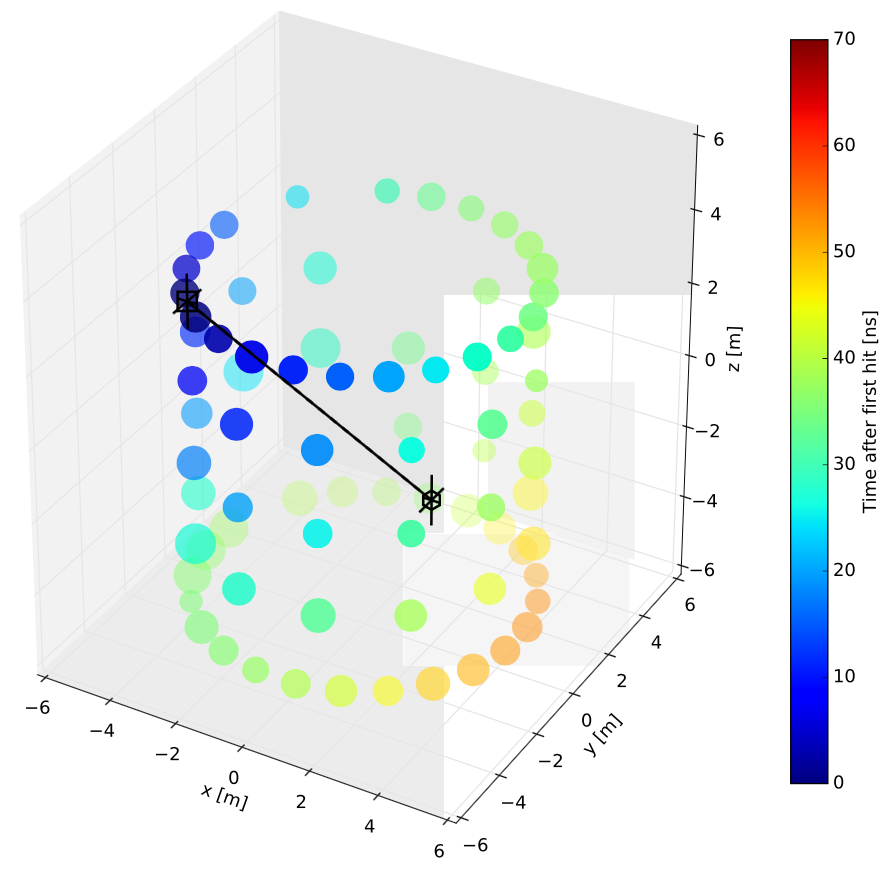
\includegraphics[width=\textwidth]{MuonVetoEvent}
\caption{Arrival time of light to muon veto PMTs helps reconstruct the muon trajectory (black line).}
\label{fig:xenon1t_water_shield_photo}
\end{figure}

\begin{figure}
\centering
\includegraphics[width=\textwidth]{InsideWaterTank}
\label{fig:xenon1t_water_shield_interior}
\end{figure}



\subsection{Calibrations}
\label{subsec:xenon1t_calibrations}
Calibrations are used for a host of purposes including understanding energy resolution, light collection efficiency, electron lifetime,
$g_1$, $g_2$, electronic and nuclear recoil bands, and many more.  Depending on the source they can be performed inside the TPC (internal) or
outside (external).  Here I cover the different calibrations and the purposes they serve; additional details and results are in
\secref{sec:det_char}.

\begin{figure}
\centering
\includegraphics[width=\textwidth]{Panoramic}
\label{fig:xenon1t_panoramic}
\end{figure}

\subsubsection{Internal}
\label{subsubsec:xenon1t_calibrations_internal}
Internal calibrations allow us to describe how our detector observes events throughout the entire TPC.  This is preferabel to external
calibrations, where only part is used.  The calibration source box is installed in the purification system (pink region in
\figref{fig:xenon1t_pur_schematic}) and contains valves opening to the GXe both before and after the getters.  When the valves are opened,
the source will flow into the GXe stream and into the cryostat and mix with the xenon.  We therefore only use sources that do not introduce
electronegative impurities.  The source will quickly spread itself throughout the entirety of the xenon, giving a uniform distribution,
and allowing us to improve our understanding of how variation in observables relates to position.

$\mathrm{^{83m}Kr}$ has two monoenergetic decays at 32.15 ($t_{1/2} = 1.83\ \mathrm{h}$) and 9.4 keV
($t_{1/2} = 154.4\ \mathrm{ns}$).  The short
half-lives coupled with its final decay product, \ce{^{83}Kr} being stable makes it a great choice to calibrate the light collection
efficiency (LCE) and measure the electron lifetime.

\radoncal is used to calibrate the ER band as \ce{^{212}Pb} - one of its daughters, is a $\beta$-emitter with endpoint energy
569.91 keV.  There are additional $\alpha$, $\beta$, and $\gamma$ emissions throughout the chain that can be used for additional studies,
including measuring the electron lifetime with the \ce{^{212}Bi} $\alpha$-decay (6.207 MeV).  The longest half-life in the chain is
\ce{^{212}Pb} with $t_{1/2} = 10.6\ \mathrm{h}$ (next longest is \ce{^{212}Bi} with $t_{1/2} = 1.00\ \mathrm{h}$), which allows DM data
to resume within several days.

Tritiated methane ($\mathrm{C H_3 T}$) is a very attractive candidate because of it's low-energy $\beta$-emission.  With a 18.6 keV
endpoint energy, it is an ideal candidate for calibrating the low-energy ($\mathrm{cS1} < 100\ \mathrm{PE}$, \textbf{check this}) ER band,
and even measuring
the light and charge yield in a relatively unexplored but important region.  This was originally done by LUX (\citeref{LUX2016}) and
subsequently performed with XENON100 (\citeref{Aprile2018}).  However, with a half-life of $t_{1/2} = 12.3\ \mathrm{y}$ it must be
removed completely by the getters to avoid introducing a new background.  This is further complicated by a suspicion that
$\mathrm{C H_3 T}$ adheres to the cryostat, prohibiting total removal.  For this reason a $\mathrm{C H_3 T}$ calibration has not yet been
conducted in XENON1T.

PMT gains are calibrated using blue LEDs at low light levels.  Unlike the previous sources this calibration is done using cables that are
carried from the data acquisition (\secref{subsec:xenon1t_daq}) into the TPC.  They are fixed at various heights and angles and flash
at periodic intervals.  The result is an SPE spectrum as shown in \figref{fig:xenon1t_pmt_spe}.

\begin{figure}
\centering
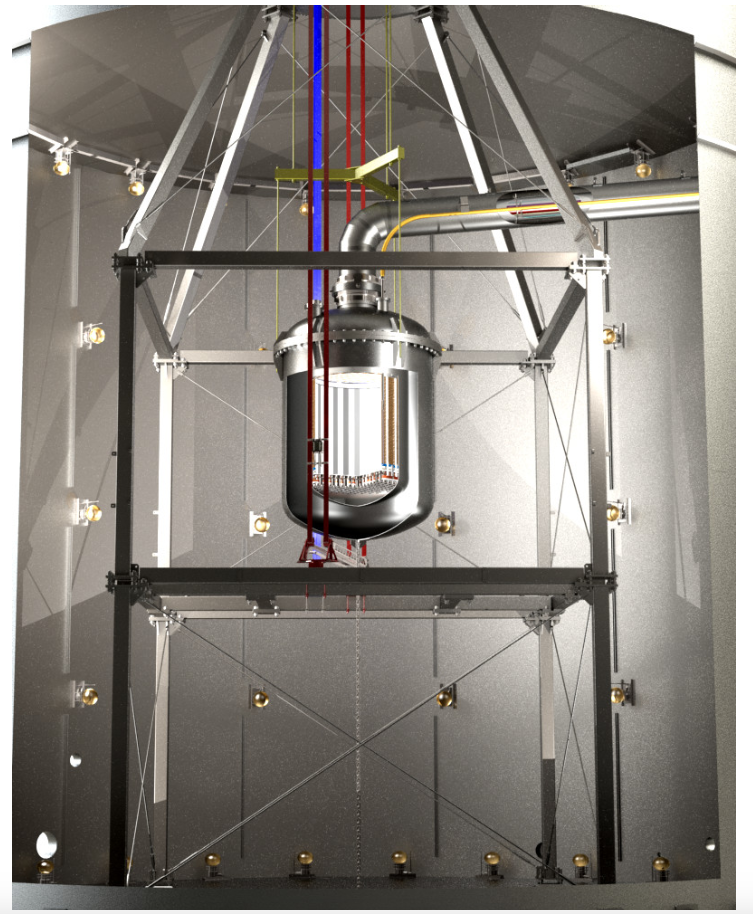
\includegraphics[width=\textwidth]{WaterTankInside}
\label{fig:water_tank_inside}
\end{figure}



\subsubsection{External}
\label{subsubsec:xenon1t_calibrations_external}
External calibrations are performed with a source outside the cryostat.  In XENON100 this was done by inserting a source inside the lead
shielding; however, the water tank in XENON1T makes this a more complicated task.  The resolution was the installation of two ``I-belts"
along the height of the detector and one ``U-belt" that also extends underneath, as shown in
\figref{fig:xenon1t_calibrations_belts}.  These
allow the sources to be lowered from the roof of the tank, as well as calibrate from different locations, so long as they are on the
belts.  They are removed during dark matter data taking.

\begin{figure}
\centering
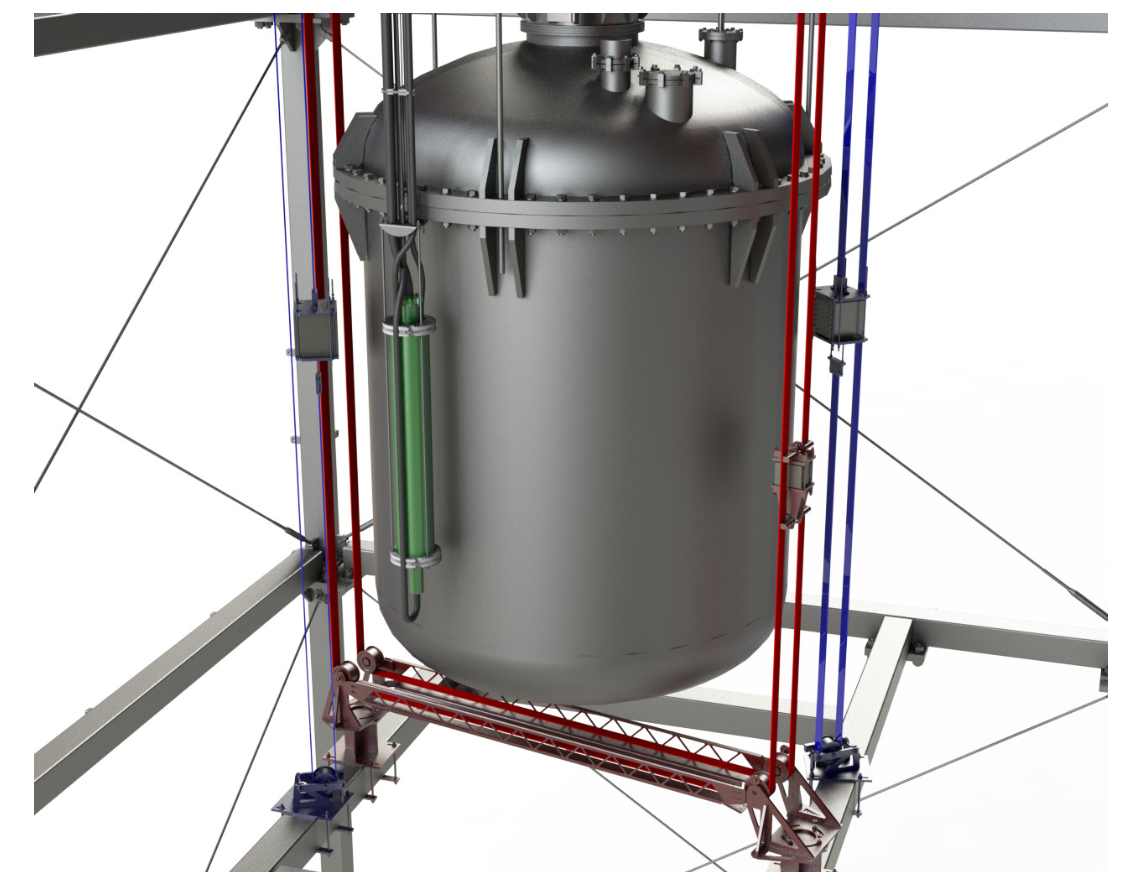
\includegraphics[width=0.8\textwidth]{TPCCalibrations}
\caption{Image credit: \citeref{Aprile2017b}.}
\label{fig:xenon1t_calibrations_belts}
\end{figure}

External $\gamma$ sources include \ce{^{137}Cs}, with an energy of 661.7 keV, and \ce{^{228}Th}, with a number of energies between 511 keV
and 2.614 MeV.  These are installed in W-collimators that restrict the \gammarays to a cone of $40^{\circ}$.  Additionally, \ce{^{60}Co}
in the cryostat flanges with 1.173 and 1.333 MeV lines can also be used.

Nuclear recoil sources \ambe and a deuterium-deuterium (D-D) neutron generator (NG) are also placed outside the TPC.  It is also deployed in a
W-collimator and emits MeV neutrons.  Details are discussed in \secref{subsubsec:er_nr_calibrations_parameter_determ_nr}.



\subsection{Data Acquisition}
\label{subsec:xenon1t_daq}
The data acquisition (DAQ) is in a temperature-controlled room on the second floor of the service building.  It can record the TPC and
muon veto PMTs either independently or simultaneously.  The signals from the TPC first pass through Phillips Scientific 776 amplifiers
where they undergo 10-fold amplitude increase.  They, along with the muon veto signals, are then digitized via 100 MHz CAEN V1724 flash
ADC boards (32 in total) that have 40 MHz bandwith, 14 bit resolution, and 2.25 V or 0.5 V, respectively.  \figref{fig:xenon1t_waveform}
shows a standard waveform recorded by the DAQ.  A single independent clock
connects to each ADC to ensure they are properly aligned and a 0.1 Hz synchronization signal is passed from a custom-developed GPS-synched
module.

\begin{figure}
\centering
\includegraphics[width=\textwidth]{Waveform}
\caption{Example of a waveform from XENON1T.  The bottom panel shows hits (red circles) observed for each PMT channel over time with
larger areas representing greater intensity.  An S1 (76.2 PE) is visible at ${\sim}380\ \mathrm{\mu s}$, marked by the blue circle in the
middle panel.  The shape of the S1 (left) and the light seen by the bottom PMT array (center right) are shown in the top panel.  At
${\sim} 1000\ \mathrm{\mu s}$ an S2 (2120.1 PE) occurs.  Its shape (center left) and light distribution in the top PMT array (right) are
shown in the top panel.  The red cross marks the $x \mdash y$ coordinates from the position reconstruction algorithm
(\secref{subsec:det_char_position_reconstruction}).  S2s are marked by
green circles in the middle panel.  We see in this waveform after the primary S2 two smaller ($< 40\ \mathrm{PE}$) S2s follow that are
$\lesssim 3\ e^-$.}
\label{fig:xenon1t_waveform}
\end{figure}

The TPC DAQ reads every pulse $> 0.3\ \mathrm{PE}$ from each PMT independently and regardless of any signal from other
channels.  The read-outs of the ADC boards are passed to six computers at up to $300\ \mathrm{MB\ s^{-1}}$ (${\sim}100\ \mathrm{Hz}$) and
are stored - along with relevant information such as time and channel - in a MongoDB database.  The sum of the bottom PMTs along with veto
and busy information is constantly read by a separate computer to determine the deadtime.  The DAQ continuously monitors data quality
parameters such as baseline, trigger, and noise.

\begin{figure}
\centering
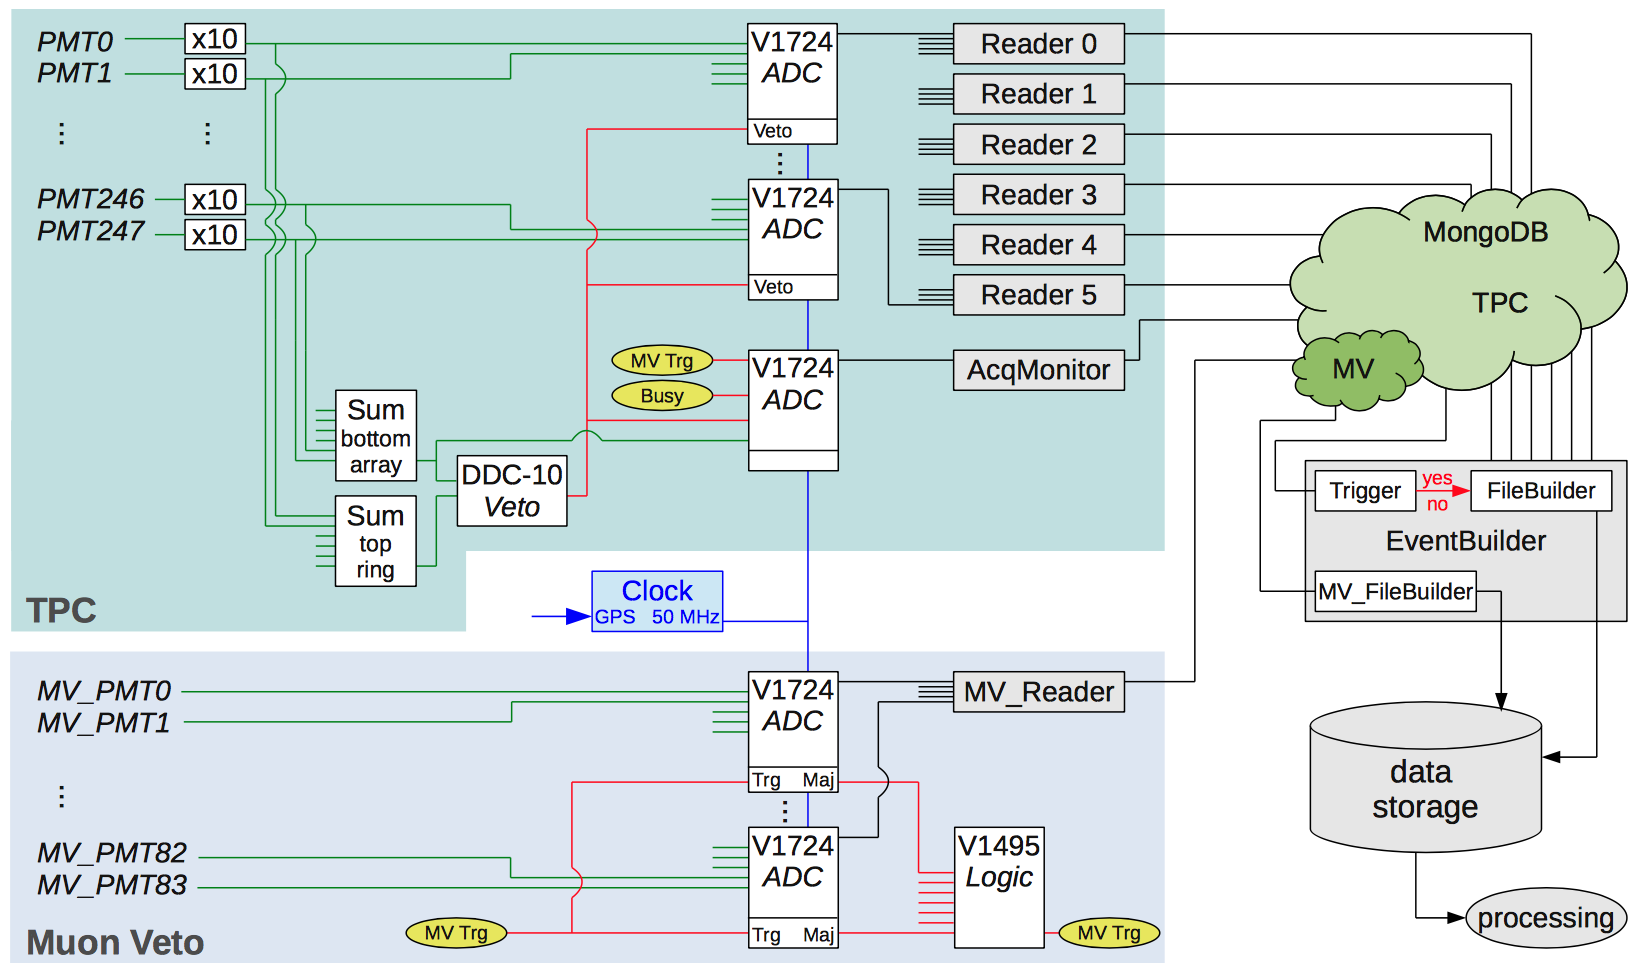
\includegraphics[width=\textwidth]{DAQ}
\caption{Schematic of the data acquisition.}
\label{fig:xenon1t_daq_schematic}
\end{figure}

A software eventbuilder on three server-grade machines decides if an interaction has occurred in real-time by examining the
time-clustering of PMT signals, and opts whether or not to trigger.  Metadata from the trigger decision is recorded and can be monitored
online to check performance or offline for analysis.  At larger than 200 PE (${\sim}7\ e^-$) the trigger efficiency is $> 99\%$.  The muon
veto uses a simple coincidence trigger that is directed by a CAEN V1495 VME unit.

Two 10 Gbps fibers transfer the raw data to buffer-storage at LNGS for temporarily housing.  The raw data is then moved to the US Open
Science Grid and European Grid Infrastructure for processing and backed up in Stockholm.  \figref{fig:xenon1t_daq_schematic} shows an
overview of the DAQ system.

To prevent acquisition of bad data four quality quality checks are performed - three of which occur in real time during data taking.  The
first is a \textit{high energy veto} that goes to \texttt{TRUE} in the event of a very large S2.  When this occurs the DDC-10 (custom
module) forwards a \texttt{NIM} pulse to the ADC boards, which blocks data from being copied to the readers.  Simultaneously a
\texttt{BUSY ACTIVE} signal is sent from the DDC-10 to the
acquisition monitor digitizer.  After 10 ms the high energy veto returns to \texttt{FALSE}, ending the \texttt{NIM} pulse and resetting
\texttt{BUSY INACTIVE}.  This mode is only used during calibrations.

Each of the 32 digitizers (aside from the DAQ monitor) feeds a low-voltage differential signaling (LVDS) pulse to the V1495 logic
module.  Each
are \texttt{TRUE} if the memory buffer is nearly full and is otherwise \texttt{FALSE}.  This is called a \textit{busy veto} and in a
similar fashion to the high energy veto,
the V1495 fans a \texttt{NIM} pulse to the digitizers to block copying of their data to the readers and sends a \texttt{BUSY TRUE} to the
DAQ monitor digitizer.  Once all digitizers return to less than full memory the veto is lifted, though it must remain active for
$\geq 10\ \mathrm{ms}$.

The final check that occurs during data acquisition is the \textit{busy type check}.  It ensures that nowhere in the event was a veto
signal, i.e. the busy signal must set to \texttt{BUSY FALSE}.  This is in part to reject events where a large S2 triggers a high energy
veto that cuts off subsequent smaller S2s (or even part of the large S2) in the same waveform.  It also cuts PMT flashes, which would
trigger a busy veto.

The final quality cut is done in processing.  On a small number of occasions events at the end of a data DAQ run some of the channels
would be missing.  To fix this the final 21 seconds of each 1 hour run are omitted from analysis.  This duration was determined by the
internal clock of the digitizers, which count from zero to 0x3FFF in 10 ns steps, or ${\sim} 21\ \mathrm{seconds}$.



\subsection{Slow Control System}
\label{subsec:xenon1t_detector_slow_control}
The subsystems are controlled, monitored, and recorded by a slow system.  The system uses General Electric (GE) Programmable
Action Controllers (PACs) and Complicity Supervisory Control And Data Acquisition (SCADA) for hardware and software, respectively.  Nearly
2500 parameters are stored in a GE Proficy Historian database, which can be queried for analysis offline.  Breach of alarm conditions
(e.g. out of range, connection loss, failure of equipment) triggers notifications via email, pre-recorded voice messages over landline,
and SMS texts to cellular phones.

Individual PACs from the GE RX3i family control sensors and actuators of the purification, cryogenics, krypton distillation,
LXe storage, and water purification systems.  The PACs connect to a private front-end network.  PAC alarms are transmitted using the
GE Alarm\&Event Express tool to the alarm system.  In addition to the SCADA system operations are possible via touch screens.  Open
Platform Communication (OPC) servers, web services, or the Modbus protocol integrate the DAQ, high-voltage supply, and calibration
system motor controllers into the slow control system.  For extra security the system requires certain conditions to be met before
performing potentially unsafe operations.

PACs and OPC servers connect to two redundant SCADA servers on the front-end network.  Two redundant fibers link the experiment to the
aboveground laboratory.  An aboveground building then houses supervisory and data storage components including the alarm system, Historian
database, slow control viewer, and primary XENON1T control room.  The slow control system is connected to a backup server outside LNGS
to prevent data loss during a laboratory network failure.  It is powered by an extended on-battery runtime
uninterruptible power supply (UPS) with generator backup.



In the
event of a very large S2 a high energy veto is set
as \texttt{TRUE}



\section{Detector Characterization}
\label{sec:det_char}
Calibrations allow detector characterization and monitoring as well as measurement of fundamental physics.  In XENON1T calibrations have
been done with $\mathrm{^{83m}Kr}$, \ce{^{222}Rn}, \ce{^{137}Cs}, \ce{^{228}Th}, americium beryllium, a neutron generator, and LEDs.
% look at http://www.uni-muenster.de/Physik.KP/AGWeinheimer/Files/theses/Bachelor_Sergej_Schneider.pdf sections 2.2 and 2.3

The most common calibration source is $\mathrm{^{83m}Kr}$.  Being a noble gas it can be injected directly into the xenon so to be used as an
internal calibration.  \ce{^{83}Rb} is installed in a source box connecting to the purification system
(\secref{subsec:xenon1t_calibrations_internal}) and decays through electron capture

\begin{equation}
\mathrm{^{83}Rb} + e^- \rightarrow \mathrm{^{83}Kr} + \nu_e
\end{equation}

\noindent with a 74.8\% branching ratio to the metastable state $\mathrm{^{83m}Kr}$.  $\mathrm{^{83m}Kr}$ then de-excites in two steps:
emission of a 32.2 keV
conversion electron with half-life $t_{1/2} = 1.83\ \mathrm{h}$ followed by a second conversion electron at 9.4 keV with
$t_{1/2} = 154.4\ \mathrm{ns}$.  The short interval between the two decays makes tagging events easy and has strong discrimination power
against nominal background.  The events that can be used for studies including detector characterization need to have both S1s resolved
by the DAQ.  To select such events the time between S1s $Delta t_{\mathrm{S1}}$ to be between 500-2000 ns $500-2000\ \mathrm{ns}$.  This
cuts more than 96\% of \metakr events but the high activity is enough to perform the studies with large
statistics.  \figref{fig:calibrations_kr_s1_s2} shows corrected and uncorrected S1s and $\mathrm{S2_b s}$ for \metakr events.  While the
$\Delta t_{\mathrm{S1}}$ cut rejects more than 96\% of \metakr events, it is extremely effective at removing background.

\begin{figure}
\centering
\includegraphics[width=\textwidth]{kr_s1_s2_cs1_cs2}
\caption{\metakr 32.2 and 9.4 keV events.  Uncorrected and corrected S1s for both decays are shown in the top left and top right
panels.  The bottom left panel shows S1 and \stwob for the 32.2 keV, and bottom right shows cS1 and $\mathrm{cS2_b}$.}
\label{fig:calibrations_kr_s1_s2}
\end{figure}

The mono-energetic lines can be used for a number of
detector characterizations including light collection efficiency (\secref{subsec:det_char_lce}), position reconstruction
(\secref{subsec:det_char_position_reconstruction}), S2 correction maps (\secref{subsec:det_char_s2_position_correction}), and electron
lifetime (\secref{subsec:det_char_elifetime}).


\subsection{PMT Gain}
\label{subsec:det_char_pmt_gain}
The charge that reaches the anode can change for a single phototube and varies between different.  Increasing the bias voltage amplifies
the gain, heightening sensitivity or conversely lowering can help prevent saturation.  Gains may also deviate from variations in
temperature (\textbf{check this}), overexposure to light, count rate, wear, and more.  Phototubes may differ from one another
for all the reasons just mentioned, as well as inevitable - however tiny - differences in parts.  Monitoring the single photoelectron (SPE)
response for each PMT then is essential for accurately reconstructing the number of photoelectrons and by extension the energy of the
event.  This is typically done with an LED inside the TPC.  Typically blue light is used since ultraviolet is unavailable, which despite
being far outside of the 178 nm range ejects a photoelectron some small fraction of the time.  Each time the LED flashes we can record the
PMTs (during normal data taking this requires a pulse larger than some threshold, \secref{subsec:xenon1t_daq}).  After a large
($\mathcal{O}(10^{5})$)
number of trials a histogram can be fit to find the SPE gain as shown in \figref{fig:xenon1t_pmt_spe}.  Note that technically the charge
is plotted but the gain is easily found as $g = \mu_{e} / e$ where $\mu_{e}$ is the mean number of \electron and $e$ is the electron charge.  We
see a large peak centered at 0 that corresponds to the baseline noise when a photoelectron is not released.  At larger gain a series of
smaller wider peaks are visible that represent integer numbers of photoelectrons, starting with 1 at the leftmost.  There is a ``shoulder"
between the baseline and first peak that cannot be explained by only considering signal from integer PEs.  As briefly mentioned in
\secref{subsec:tpcs_pmts} this comes from photons that pass through the photocathode and free an electron on the first dynode, causing an
under-amplified charge.  This is generally the most challenging aspect to model.

\begin{figure}
\centering
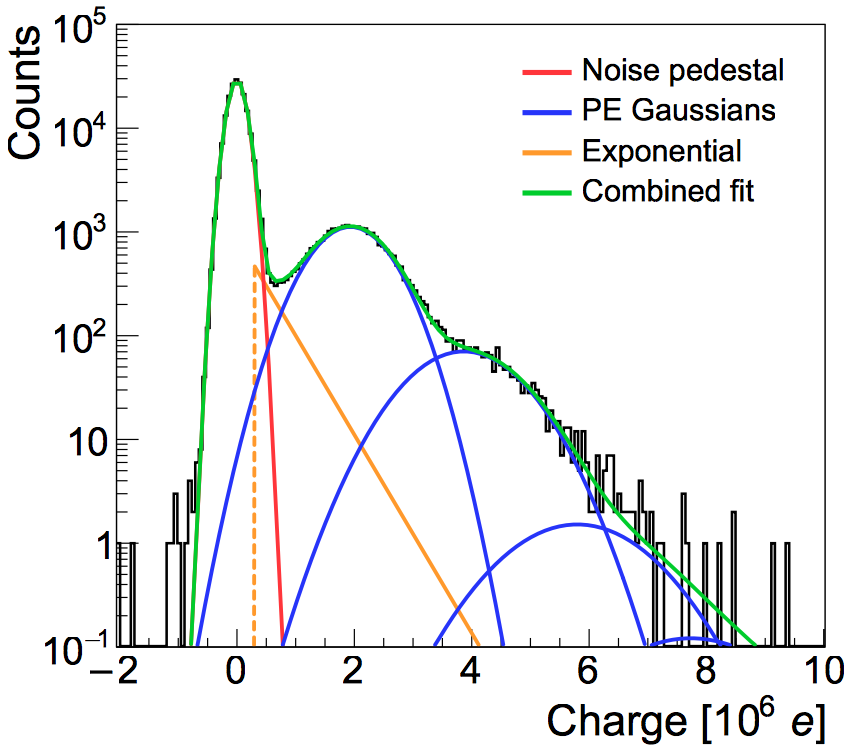
\includegraphics[width=0.6\textwidth]{SPESpectrum}
\caption{(Left) Single photoelectron spectrum.}
\label{fig:xenon1t_pmt_spe}
\end{figure}

In \figref{fig:xenon1t_pmt_spe} the spectrum is fit assuming the noise baseline and PE peaks are gaussian and the under-amplification is
an exponential.  The PE gaussians are constrained by $\mu_{N} = N \mu_{e}$ and $\sigma_{N} = \sqrt{N} \sigma_{e}$ where $\sigma_{e}$ is the
standard deviation of the single photoelectron peak and $\mu_{N}$ and $\sigma_{N}$ are the mean and standard deviation for the peak with
$N$ photoelectrons.  As this model is simplistic and can add bias recent efforts have gone in to alternative methods
of characterization (\secref{Saldanha2017, 2017Anthony}).  Nonetheless, the combined fit (green) appears to agree will with the data.

We can use the SPE spectrum to calculate the resolution $R = \sigma_{e} / \mu_{e}$.  As the gain grows the resolution should sharpen
initially until it eventually levels off.  For the R11410-21 models the plateau began around $2 \mdash 3 \times 10^{6}$ at a resolution of
27\%.  Because the stress on the PMT raises with bias voltage and larger gains lead to greater saturation we decided there was no benefit
to exceeding this gain.

\begin{figure}
\centering
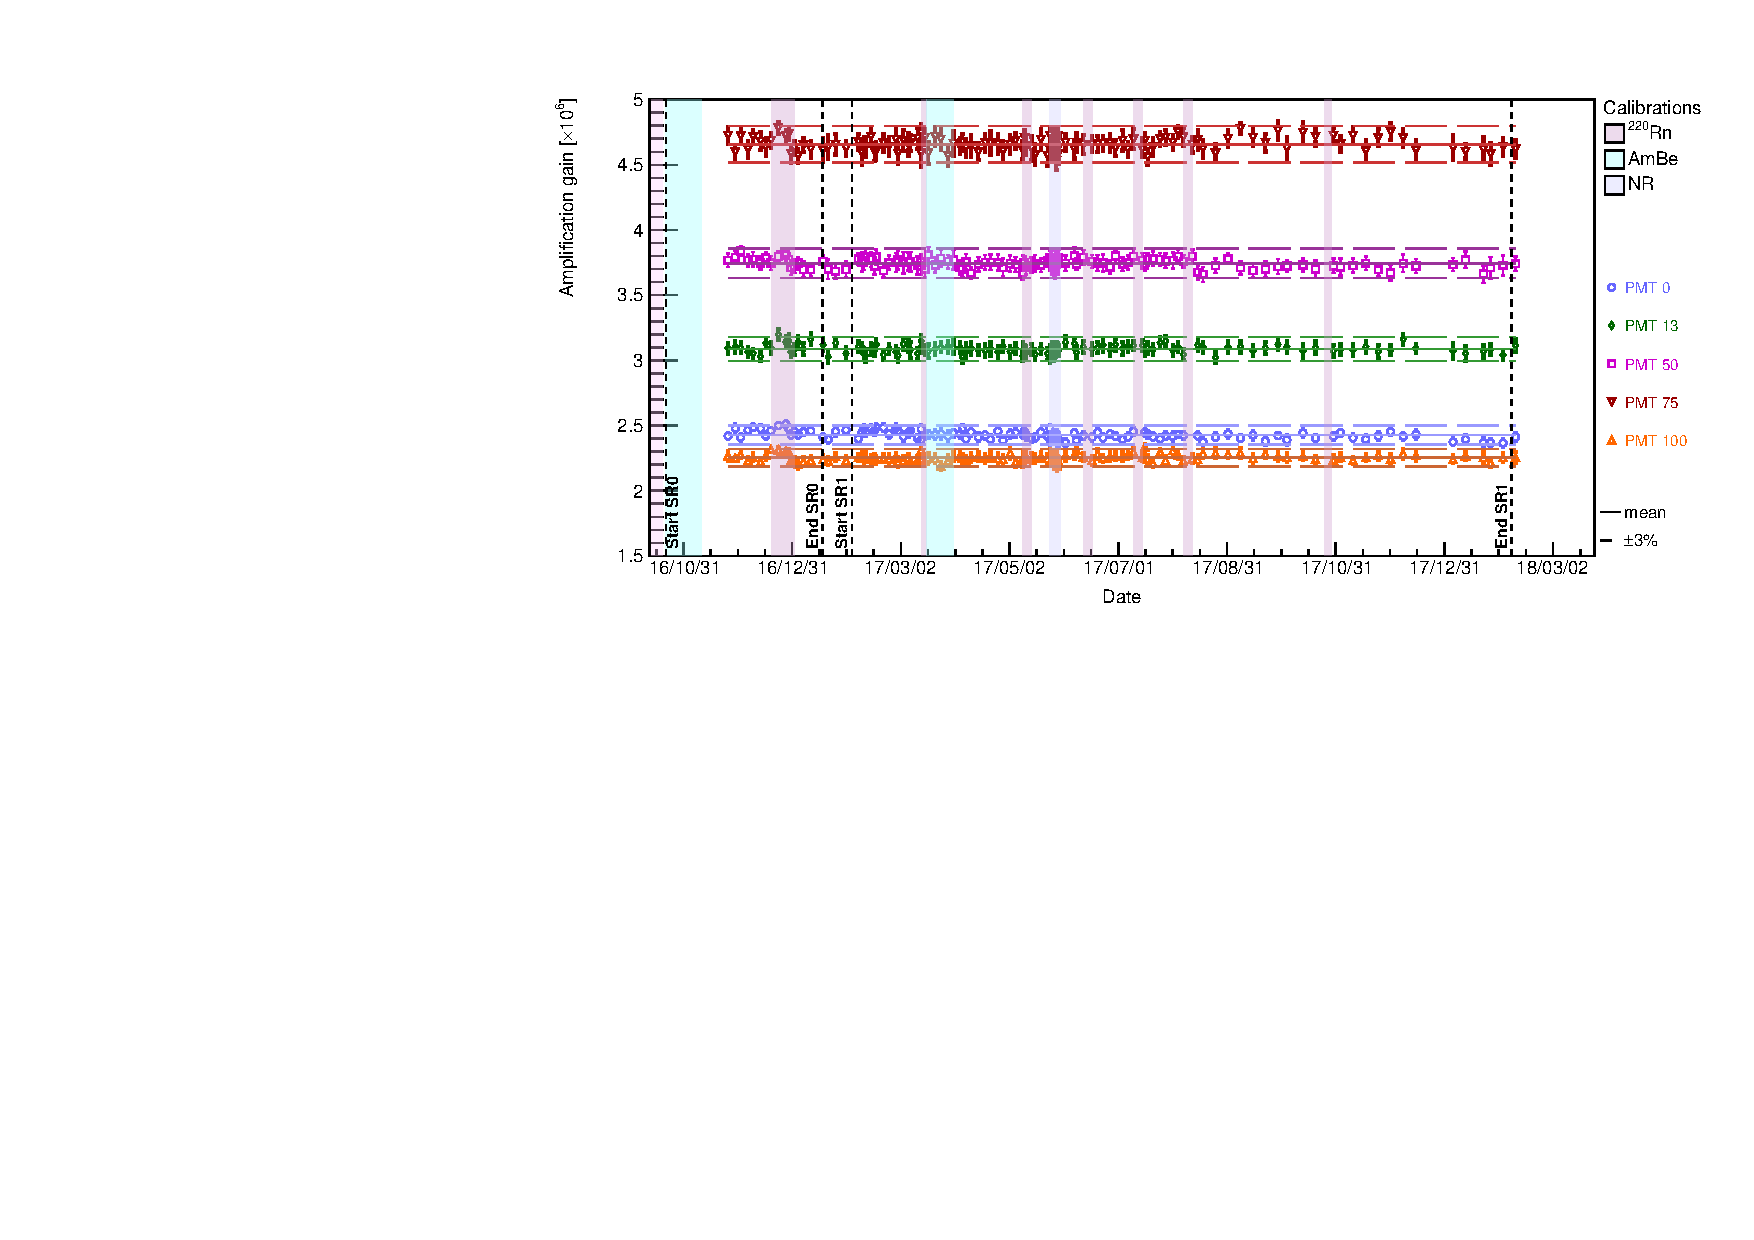
\includegraphics[width=\textwidth]{PMTGainStability}
\caption{Gains for five PMTs monitored from SR0 until the end of SR1.  Means and $\pm 3\%$ are shown.  All appear to be stable.}
\label{fig:xenon1t_pmt_time}
\end{figure}

The relatively poor resolution is apparent in \figref{fig:xenon1t_pmt_spe} as the photoelectron peaks are hard to distinguish.  An
important metric of the SPE spectrum is the peak-to-valley ratio, which divides the first PE peak by the valley that sits between it and
the baseline noise.  As with $R$ it increases for low gains and eventually levels.  For gains of $2 \mdash 3 \times 10^{6}$ the mean
peak-to-valley ratio is ${\sim} 3$.  The PMT gains are regularly measured to identify any changes in gain.  This is shown for five
PMTs - all of which are stable - in \figref{fig:xenon1t_pmt_time}.



\subsection{Light Collection Efficiency}
\label{subsec:det_char_lce}
The light observed by a PMT depends on - among other things - the position of the event.  The light collection efficiency (LCE),
$\mathcal{C}_{\mathrm{lce}}(x, y, z)$ - seen in \figref{fig:calibrations_lce_polar} - quantifies these differences.  Such
position-dependent variations exist simply because the location of
the interaction dictates subsequent effects due to detector features and physics.  First, the the solid angle of an event is not uniform
throughout the detector.  It is greatest near the bottom or top of the TPC at small radii.  The measured strength of the scintillation
from the S1 depends then on the number of PMTs the light can reach and how far the light must travel to each.  Interactions near the
wall have a lower observed intensity because of this.  The quantum efficiency (QE) of the PMTs (\figref{fig:xenon1t_pmt_array}) is also a
factor, with those at larger values more likely to produce a photoelectron.  Because the PMTs with the highest QE were placed in the
center of the bottom array (\secref{subsec:xenon1t_pmts}) events that happen near there should have a higher likelihood of detection,
while those in in near the top corners should have the lowest.

Because PTFE has some small but $> 0$ absorption the intensity of the scintillation decreases with each reflection.  Therefore light
that is emitted perpendicular to the PMT arrays can be severely dampened.  This is amplified by the absorption of light by
impurities in the LXe, meaning that longer traversed distances imply decreased scintillation.

The index of refraction of LXe ${\sim} 1.7$
gives a critical angle $\theta_c = 36^{\circ}$.  The light then that reaches the top PMTs for an event at
$z = -10\ \mathrm{cm}$ is restricted to a radius of just 13.6 cm at the liquid surface, with the total solid angle from
$r = 0\ \mathrm{cm}$ of $83.9^{\circ}$.  While the light will be internally reflected and progress towards the bottom array, it is likely
to be lessened from reflections with the PTFE and extended travel distances as discussed in the previous paragraph. In comparison light
directed towards the surface from an event 10 cm above the cathode ($r = 0$)
has $\theta < \theta_c$ everywhere.  Some scintillation that reflects off the PTFE on the way up will rebound off the surface, but its
contribution is relatively small.

\begin{figure}
\centering
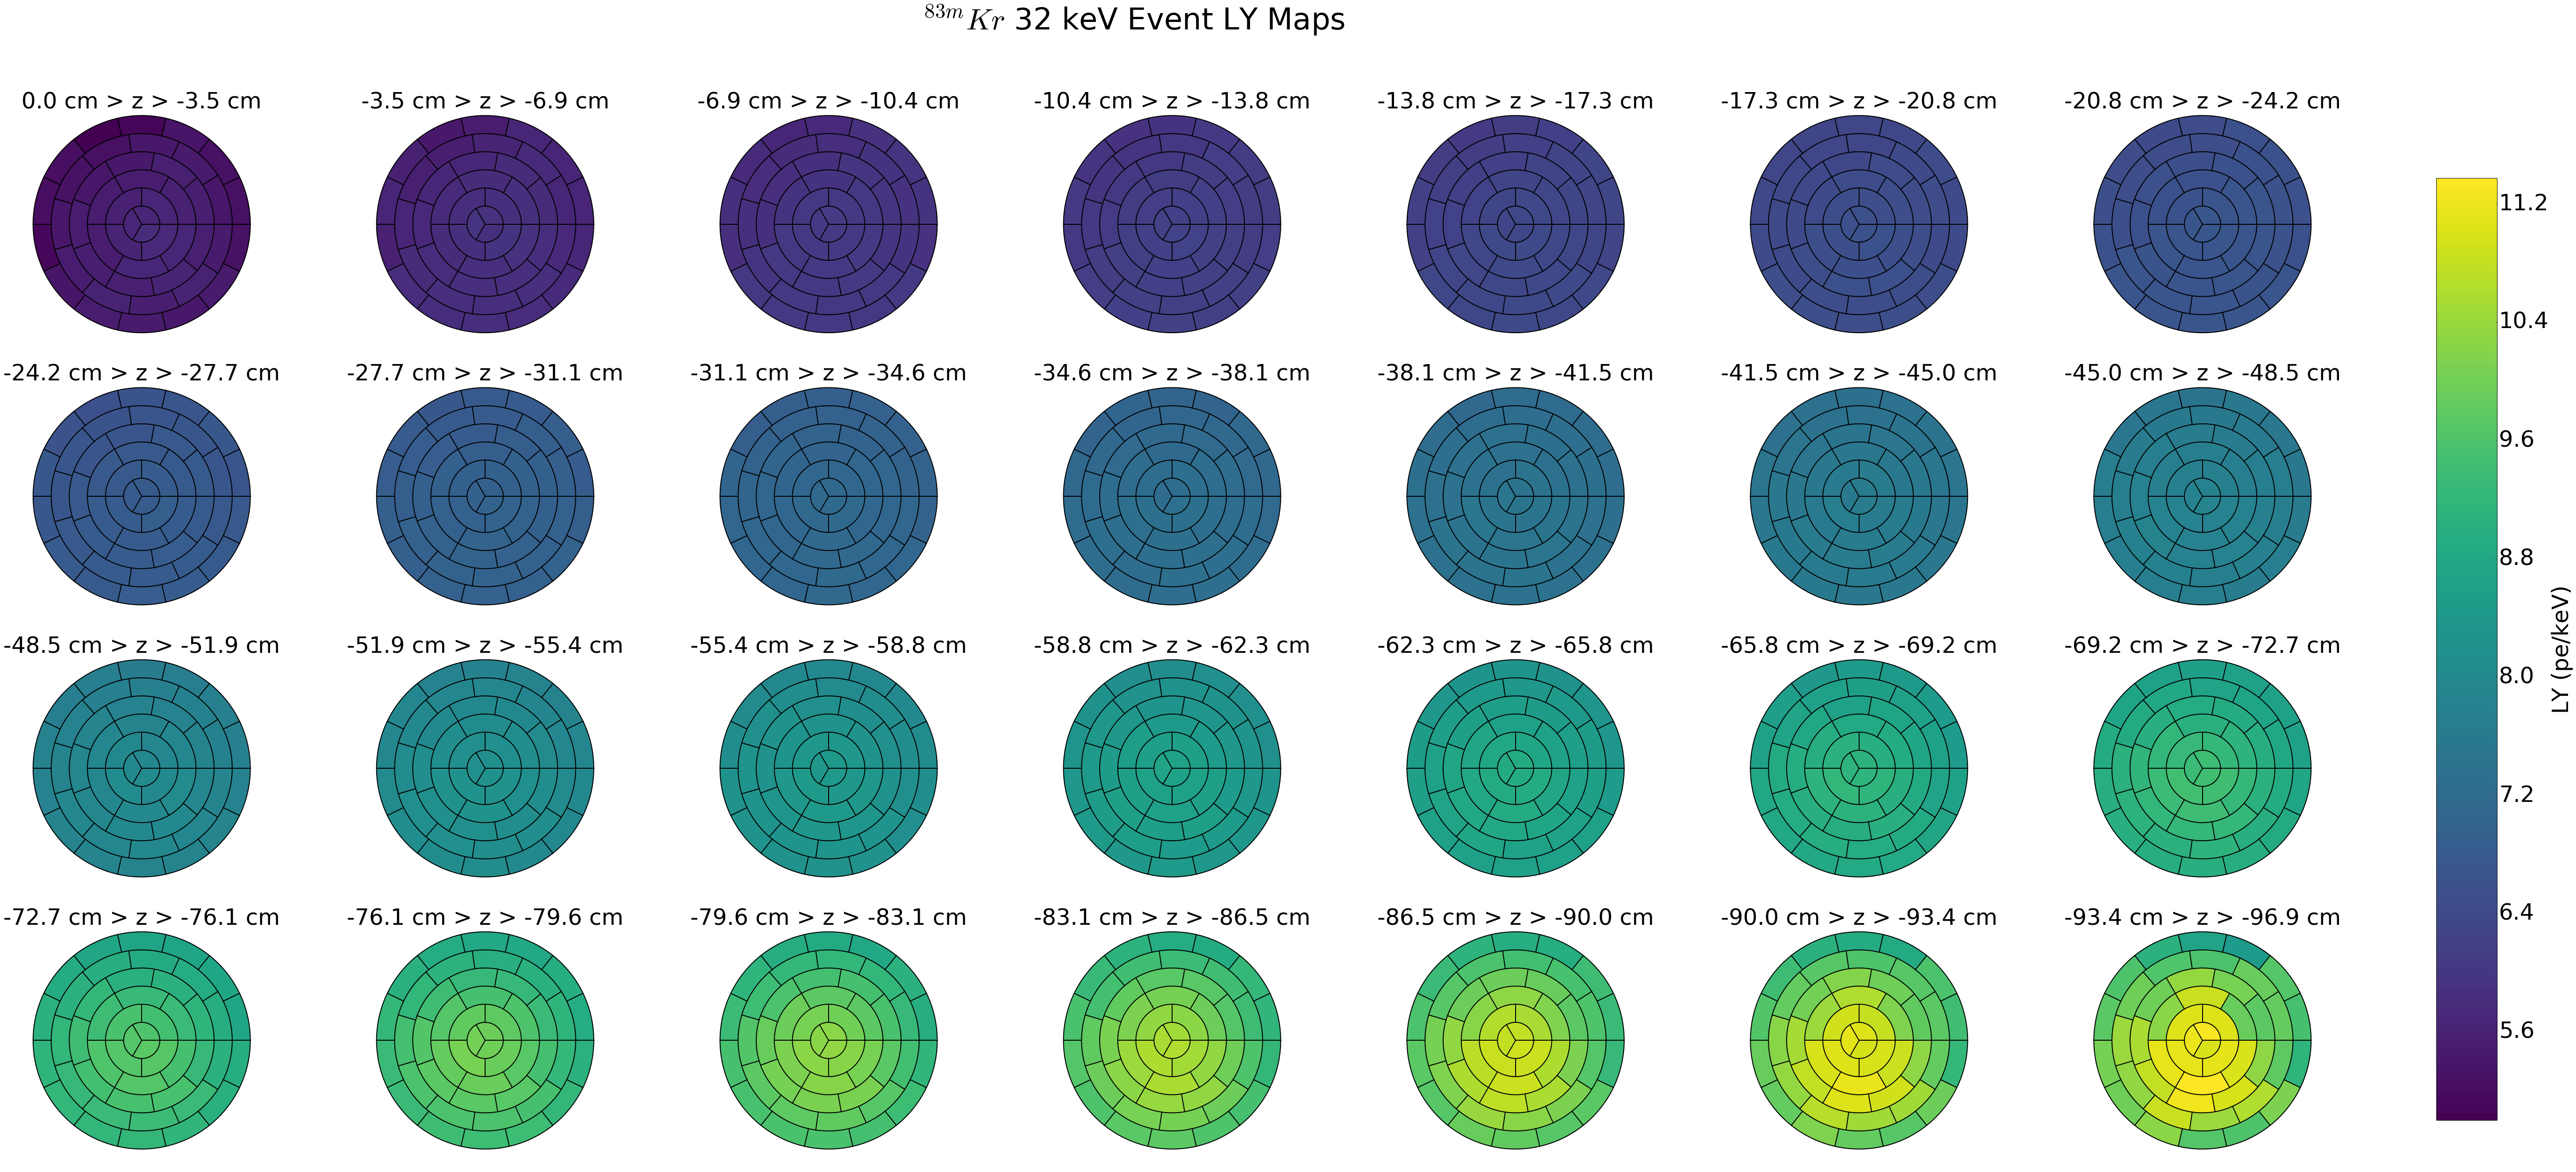
\includegraphics[width=\textwidth]{LCEMapPolar}
\caption{Light yield in slices of $z$ and $\phi$.}
\label{fig:calibrations_lce_polar}
\end{figure}

Calibrating the LCE requires a mono-energetic peak - preferably one near our DM energy range.  For this we use the light from the
$\mathrm{^{83m}Kr}$ 32.1 keV conversion electron.  The left panel in \figref{fig:calibrations_lce_lce} shows fits to S1s measured below the gate
(red), in the TPC center (blue), and above the cathode (green).  The mean from these fits correspond to the values shown in the right
panel.

It is important to point out that because recombination depends on recoil energy and electric field the derived LCE map is not
technically correct for other energies.  However, field non-uniformities are small, especially after more than a few cm inside of the
wall, so applying it universally is acceptable.

In the case of high-energy events PMT saturation can
affect the measured signal so the latter becomes important.



\subsection{Position Reconstruction}
\label{subsec:det_char_position_reconstruction}
TPCs allow 3-dimensional position reconstruction.  Since the drift velocity $v_d$
is constant in LXe the depth is easily found as $z = -v_d t_d$ where $t_d$ is the drift time ($z$ is defined to be negative with
$z = 0$ at gate).  The drift fields for SR0 and SR1 were $E_d = 118.6\ \mathrm{V\ cm^{-1}}$ and $81.3\ \mathrm{V\ cm^{-1}}$,
respectively, with $2.2\ \mathrm{V\ cm^{-1}}$ RMS variations.  The fields correspond to drift velocities of
$v_d = 1.440\ \mathrm{mm\ \mu s^{-1}}$ and $1.332\ \mathrm{mm\ \mu s^{-1}}$ and
maximum drift times of $t_{d, \mathrm{max}} = 672.8\ \mathrm{\mu s}$ and $727.3\ \mathrm{\mu s}$ (TPC drift length is 96.9
cm at$-100^{\circ}\ \mathrm{C}$).

The $x \mdash y$ coordinates are found by applying an algorithm to the intensity each PMT in the top array observed from the S2 (also known as
PMT hit pattern).  For XENON1T two reconstruction algorithms were mainly used.  The first was a neural net using the Fast Artificial
Neural Network (FANN) library with 24 and 29 nodes in the two hidden layers (sequentially).  The second matches the real hit pattern with
an expected after weighting four other algorithms for its seed, and is known as top pattern fit (TPF).  Both algorithms were trained on MC
and optimized with $\mathrm{^{83m}Kr}$ data, and achieved a position resolution of $\lesssim 2\ \mathrm{cm}$.  For SR1 the NN was ultimately
chosen, as the TPF algorithm was more sensitive to dead PMTs and showed some artificial discontinuity in the radial
direction.  \figref{fig:calibrations_position_reconstruction} shows the position distribution of events in SR1 along with the 1 ton FV
that was used in originally used in the SR0-only results (\citeref{Aprile2017f}), the 1.3 t used in SR1, and the active volume.

To determine position reconstruction $\mathrm{^{83m}Kr}$, \ce{^{214}BiPo}, wall samples, and MC are used.

\begin{figure}
\centering
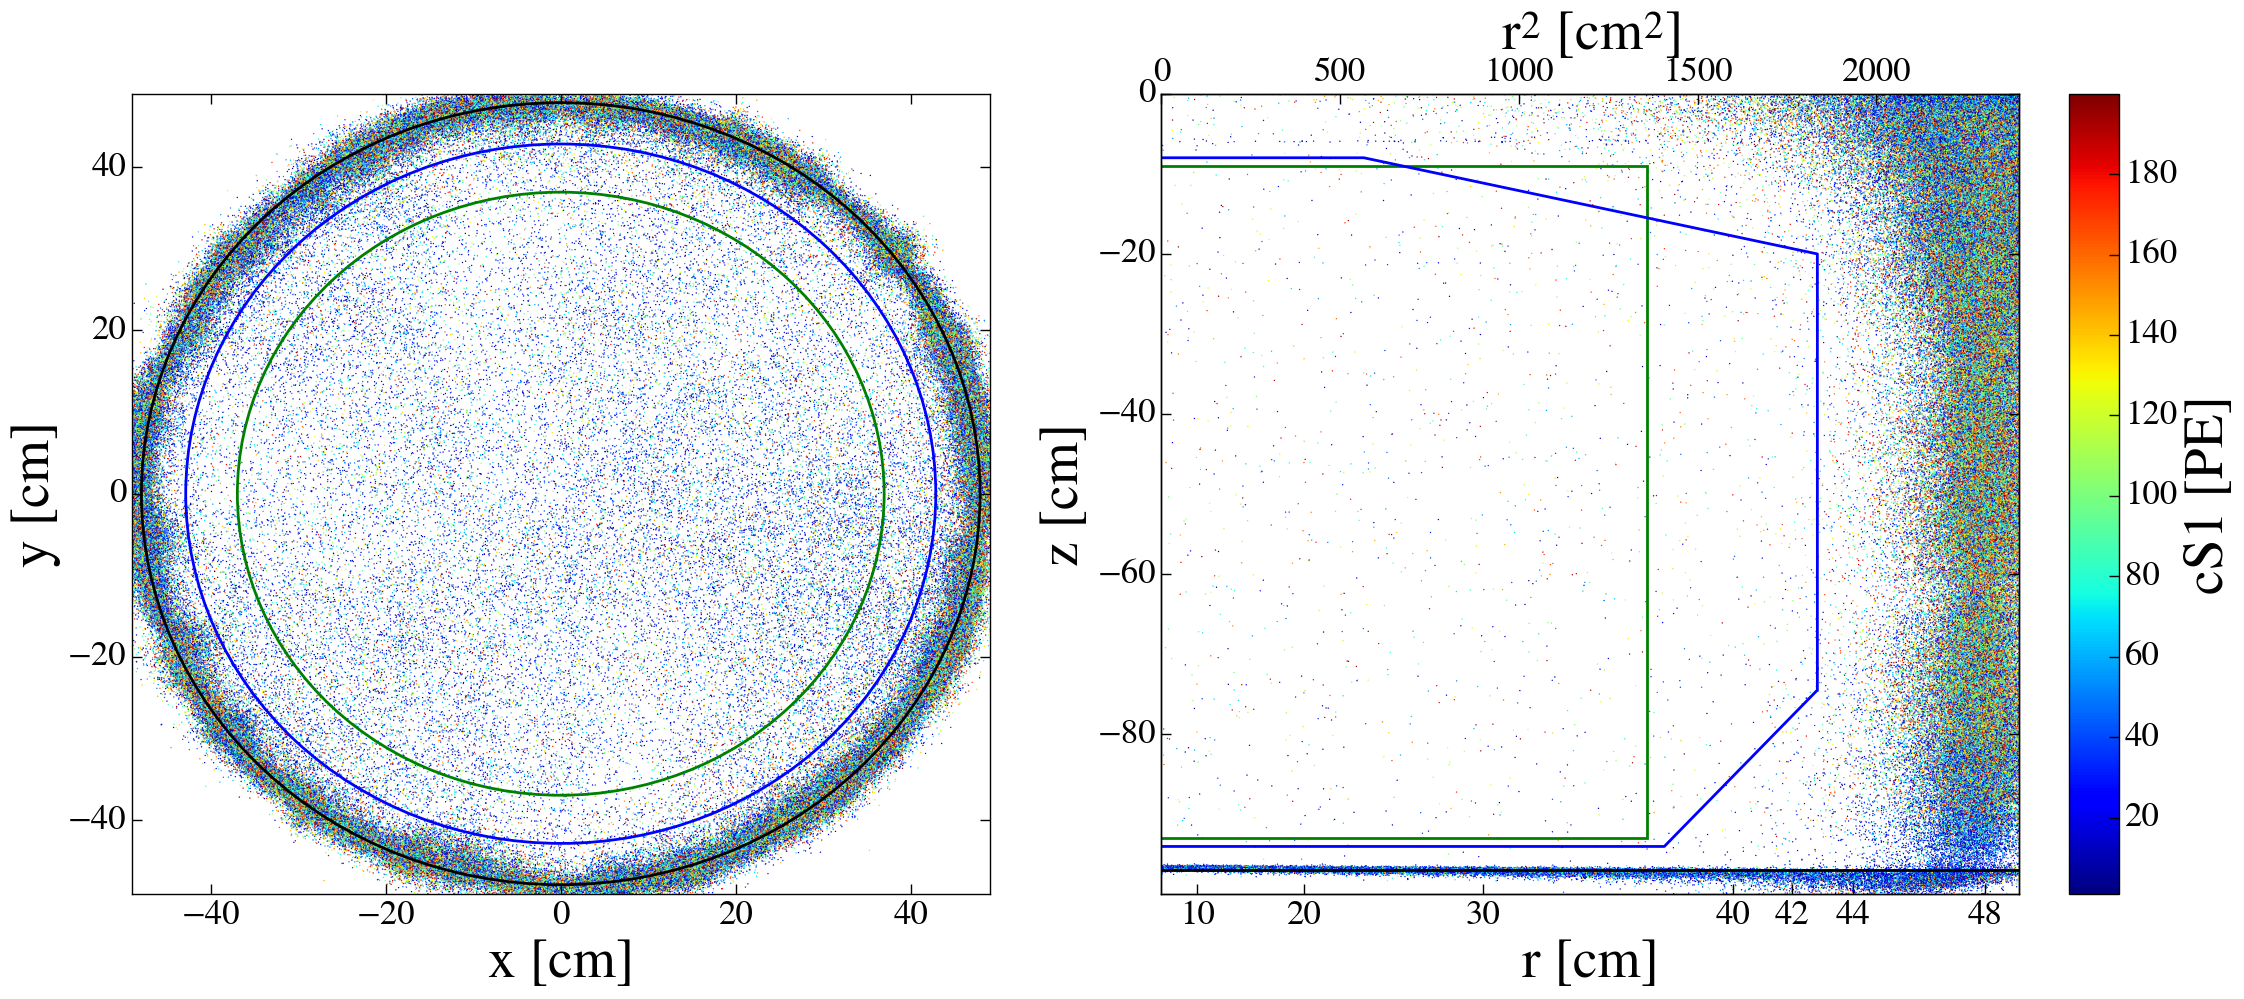
\includegraphics[width=\textwidth]{FVBoth}
\caption{Positions of background events plotted in $x$ vs. $y$ and $r$ ($r^2$) vs. $z$ for SR1.  The 1 ton FV originally used
in the SR0-only is shown in green and defined by $-92.9 < z < -9\ \mathrm{cm}$, $r < 36.94\ \mathrm{cm}$.  The 1.3 ton FV for SR1 is
outlined in
blue, with the maximum radius plotted in the left panel.  Its shape is more complicated but has $z_\mathrm{min} = -94\ \mathrm{cm}$,
$z_{\mathrm{max}} = -8\ \mathrm{cm}$, and $r_{\mathrm{max}} = 42.84\ \mathrm{cm}$.  The active volume (surrounded by the cathode, wall,
and gate) is marked in black.  The events that appear outside the wall are wall events that were not properly
reconstructed.  The events below the cathode result from field inhomogeneities that lead to extended drift times, which is why they
become more exaggerated towards the bottom corner of the TPC.}
\label{fig:calibrations_position_reconstruction}
\end{figure}

An important consideration is how close to the true position do we get when we reconstruct.  In regions underneath dead or malfunctioning
PMTs the position resolution is significantly worse.

\begin{figure}
\centering
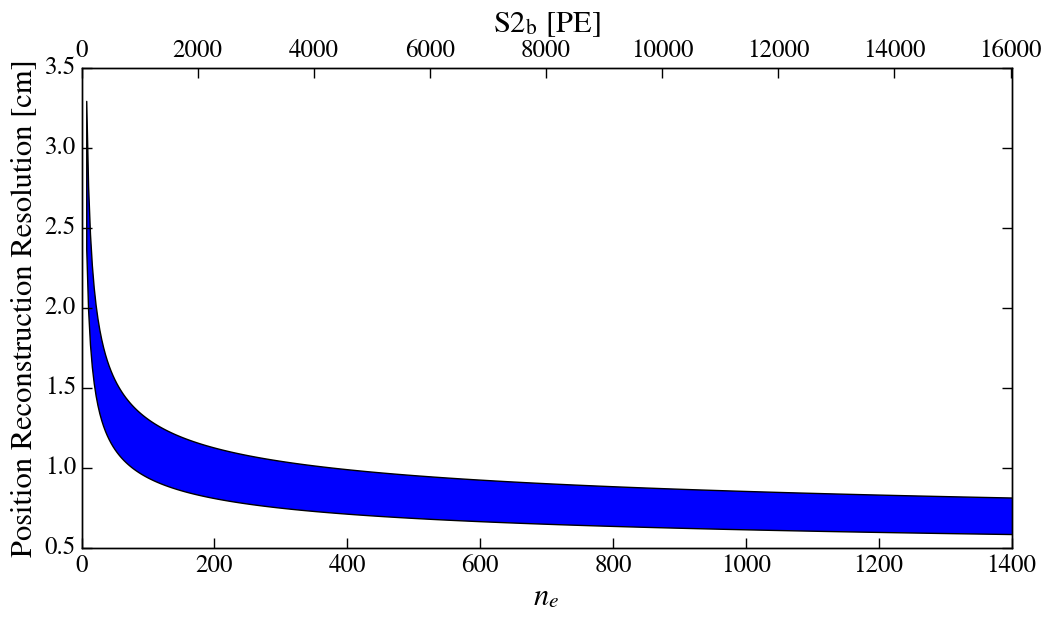
\includegraphics[width=\textwidth]{PosRecRes}
\caption{Position reconstruction resolution for for SR1 as a function of number of electrons and $\mathrm{S2_b}$.  At lower $n_e$ the
resolution becomes much worse due to the limited S2 scintillation seen by the top PMTs.  At low-energies ($n_e \lesssim 100\ e^-$,
$\mathrm{S2_b} \lesssim 1000\ \mathrm{PE}$) the position resolution becomes extremely poor.  Note that this refers only to $x \mdash y$
($(\Delta x^2 + \Delta y^2)^{0.5}$), as the drift time should almost always allow precise $z$-reconstruction.}
\label{fig:calibrations_position_reconstruction_res}
\end{figure}



\subsection{S2 $\mathbf{x \mdash y}$ Correction}
\label{subsec:det_char_s2_position_correction}
We must also account for $x$ and $y$ variations in S2 (the $z$-correction is calculated using the electron lifetime in
\secref{subsec:det_char_elifetime}).  For
this we use the 41.5 keV peak of $\mathrm{^{83m}Kr}$ (the 154 ns half-life of the 9.4 keV decay makes it difficult to separate the two
S2s).  Most of the light seen by the top array is focused on a small group of PMTs directly over the extraction site, while a large
solid angle causes a more uniform spread on the bottom array.

The top and bottom correction maps are shown in \figref{fig:calibrations_s2_maps}.  The relative S2 light yield is shown, which can be
thought of as variations on $g_2$ or the single electron gain $G_e$ (\secref{subsec:det_char_single_electron_gain}).  The local
fluctuations are primarily the result
of nonfunctional PMTs.  The observed signal in the top array being more densely concentrated causes steeper local variations.  The
slightly higher S2s at low radii result from a small sagging of the anode.  The increase in the bottom array as $r \rightarrow 0$ is 
mainly due to the higher QE.  The large solid angle creates a roughly homogeneous azimuthal distribution.

\begin{figure}
\centering
\includegraphics[width=\textwidth]{s2_relative_light_yield}
\caption{Relative S2 light yield for the top (left) and bottom (right) PMT arrays.  Light from \electron extracted across the GXe is
concentrated in the PMTs directly above it in the top array.  Large fluctuations in the top array are due primarily to dead PMTs while
smaller are from variation in gains.  A larger solid angle results in a more uniform distribution across $\phi$ in the bottom array.}
\label{fig:calibrations_s2_maps}
\end{figure}

Of course the position must be reconstructed (\secref{subsec:det_char_position_reconstruction}) before any correction can be
applied.  Thus events that have poor position resolution (mainly either below dead PMTs or low-energy) have a higher chance of being
more greatly miscorrected.



\subsection{Electron Lifetime}
\label{subsec:det_char_elifetime}
The electron lifetime $\tau_{e}$ (see \secref{subsec:tpcs_working_principle} for impurity attachment details) quantifies the charge $q$
that is lost as it drifts to the liquid-gas interface.  It is given by

\begin{equation}
q(t_d) = q_0 e^{-t_d / \tau_{e}}
\label{eq:det_char_elifetime}
\end{equation}

\noindent where $q_0$ is the charge that escapes recombination.  Generally when calculating $\tau_{e}$ a mono-energetic source is used so
that $q_0$ is the same throughout the detector.  During dark matter data taking the electron lifetime is monitored through background
\ce{^{222}Rn} and \ce{^{218}Po} $\alpha$-decays.  Because materials with low \ce{^{222}Rn}
emanation were chosen, electron lifetime measurements usually required 24-48 hours of data.  Alternatively, calibrations can
have significantly higher (${\sim}50\ \mathrm{Hz}$) statistics, allowing measurements with significantly greater precision.

The 32.2 keV $\mathrm{^{83m}Kr}$ de-excitation provides an electronic recoil to measure $\tau_{e}$.  The total number of events
from a typical calibration of 2-3 days is in the millions, and even with $< 4\%$ acceptance of \metakr events the number of usable events
is ${\sim}10^5$, making any contamination from background
negligible.  \figref{fig:det_char_elifetime_kr} shows an electron lifetime calculated using $\mathrm{^{83m}Kr}$.

\begin{figure}
\centering
\includegraphics[width=\textwidth]{kr_electron_lifetime_linear}
\caption{The model is derived using \ce{^{222}Rn}, \ce{^{220}Rn}, and \ce{^{218}Po} \alphadecays and
discussed in \chapref{chap:purification}.}
\label{fig:det_char_elifetime_kr}
\end{figure}

Another high-statistic calibration used for measurement is \ce{^{220}Rn}.  Primarily used for the 569.9 keV $\beta$-emission of its
decay chain daughter \ce{^{212}Pb} (\secref{subsubsec:er_nr_calibrations_parameter_determ_er}), a number of elements along the chain
undergo $\alpha$-decays that can be
used.  \tabref{tab:alpha_decays} lists the main $\alpha$-emitters in both the \ce{^{222}Rn} and \ce{^{220}Rn} chains.  Because calibration
data is only used after the source valve is closed, the 55.6 s and 145 ms half-lives of the first two $\alpha$-emitters \ce{^{220}Rn} and
\ce{^{216}Po}, respectively cannot be used.  However \ce{^{212}Bi} releases a 6.207 MeV $\alpha$ in its decay to \ce{^{208}Tl} with a
branching ratio of 36.9\%.  A typical electron lifetime using \ce{^{212}Bi} is shown in the right panel of
\figref{fig:calibrations_elifetime}.

Other sources can be used for measuring $\tau_{e^-}$ but with less success.  In past experiments the 661.7 \gammaray of \ce{^{137}Cs} was
used, but an early trial in XENON1T showed that very few actually reached the active volume, making the method inefficient.  Additionally
the 163.9 and 236.1 keV de-excitations of $\mathrm{^{131m}Xe}$ and $\mathrm{^{129m}Xe}$, respectively, following a nuclear recoil calibration are
usable initially but longer time windows are required as they de-excite, and they do not offer the large statistics of $\mathrm{^{83m}Kr}$
or \ce{^{220}Rn}.

\bgroup
\def\arraystretch{1.2}
\begin{table}
\centering
\begin{tabular}{cccccc}
\hline
Isotope & Daughter & Energy & $t_{1/2}$ & Chain \\
\hline
\ce{^{222}Rn} & \ce{^{218}Po} & 5.590 MeV & 3.82 d & \ce{^{222}Rn} \\
\ce{^{218}Po} & \ce{^{214}Pb} & 6.115 MeV & 3.10 m & \ce{^{222}Rn} \\
\ce{^{214}Po} & \ce{^{210}Pb} & 7.833 MeV & $164.3\ \mathrm{\mu s}$ & \ce{^{222}Rn} \\
\ce{^{210}Po} & \ce{^{206}Pb} & 5.407 MeV & 138.4 d & \ce{^{222}Rn} \\
\ce{^{220}Rn} & \ce{^{216}Po} & 6.405 MeV & 55.6 s & \ce{^{220}Rn} \\
\ce{^{216}Po} & \ce{^{212}Pb} & 6.906 MeV & 145 ms & \ce{^{220}Rn} & \\
\ce{^{212}Bi} & \ce{^{208}Tl} & 6.207 MeV & 1.01 d & \ce{^{220}Rn} & \\
\ce{^{212}Po} & \ce{^{208}Pb} & 8.954 MeV & 299 ns & \ce{^{220}Rn} & \\
\hline
\end{tabular}
\caption{$\alpha$-decays with high likelihoods for \ce{^{222}Rn} and \ce{^{220}Rn} decay chains.  \ce{^{222}Rn} makes up part of our
background so it an \ce{^{218}Po} are used to continually monitor the $\tau_{e^-}$.  The \ce{^{220}Rn} content in our background is
insignificant but it is used in calibrations, where \ce{^{212}Bi} allows high-statistic measurement.  Those with $< 0.1\%$ probability
(\ce{^{218}At}, \ce{^{218}Rn}, \ce{^{214}Bi}, \ce{^{210}Pb}, \ce{^{210}Bi}, \ce{^{209}Bi} for \ce{^{222}Rn} chain, \ce{^{220}Ra} and
\ce{^{216}Rn} for \ce{^{220}Rn} chain) are not listed.}
\label{tab:alpha_decays}
\end{table}
\egroup

\begin{figure}
\centering
\includegraphics[width=\textwidth]{electron_lifetime_evolution_2017_01_28_to_2018_02_20_kr_only}
\caption{Electron lifetime over SR1.  Markers represent lifetime measurements using $^{83\mathrm{m}}\mathrm{Kr}$.  The green line
and shaded region represent the median and 68\% percentiles of the best-fit model.  The voltage was lowered in early July to wash the
gate, releasing impurities into the LXe.  The model is derived using \ce{^{222}Rn}, \ce{^{220}Rn}, and \ce{^{218}Po} \alphadecays and
discussed in \chapref{chap:purification}.}
\label{fig:det_char_elifetime_evolution}
\end{figure}

The electron lifetimes from $\alpha$-decays was observed to be smaller than using $\beta$s or $\gamma$s.  While $\alpha$ energies are
significantly higher the charge yield is extremely low (\figref{fig:tpcs_signals_drift_field}).  Because our sensitive region is at
low-energy and is not affected by $\alpha$ interactions we decided to use the electron lifetime derived from $\mathrm{^{83m}Kr}$.  The
electron lifetime used for Science Runs 0 and 1 is shown in \figref{fig:det_char_elifetime_evolution}.  The flatness in $\tau_{e^-}$
may be indicative of a small leak as mentioned in \secref{subsubsec:backgrounds_electronic_krypton}.  Details on the electron
lifetime model are discussed in \chapref{chap:purification}.



\subsection{Secondary Scintillation Gain}
\label{subsec:det_char_single_electron_gain}
In measuring the S2 we know the total number of photoelectrons freed from the photocathodes of the PMTs.  However, our parameter of
interest is the number of \electron that were extracted across the GXe.  To convert between the two we need to measure the number of
detected photons per $e^-$, also known as the \textit{secondary-scintillation gain}, or \textit{single electron gain} $G_e$.  To do so we
look at the
smallest features in the waveforms of events that have the width of an S2, and therefore must be a low integer of $e^-$.  These generally
result
from photoionization of detector metals such as the gate or cathode, photoionization of impurities in the LXe, and delayed extraction
of \electron from the liquid.

The number of photons emitted depends on - among other things - the electric field between the anode and gate $E_g$.  Details of the
relation can be found in \secref{subsec:tpcs_working_principle} and \eqnref{eq:electronlum}.  The sagging - although small - of the
anode changes $E_g$ slightly along $r$ as mentioned in \secref{subsec:det_char_s2_position_correction} and shown in
\figref{fig:calibrations_s2_maps} (top).  Additionally the dielectric constant of LXe and GXe are different, so a change in liquid level
would cause a nonuniform shift in field, so is monitored over the course of data taking.

Poisson processes give a good approximation to both $G_e$ and the number of photons detected by the PMTs.  Effects like variation in $E_g$
and PMT detection efficiencies apply a smearing.  The single electron spectrum can be modeled as

\begin{equation}
\frac{1}{1 + e^{-(x - A) / B}}\ \sum_{k = 1} h_k\ \mathrm{exp} \bigg( -\frac{(x - k \mu_1)^2}{2 k \sigma_1^2} \bigg)
\label{eq:det_char_single_electron_gain_model}
\end{equation}

\noindent where $x \equiv \mathrm{S2}$.  Each term in the sum refers to the peak composed of $k$ electrons with amplitude $h_k$.  The
peaks are assumed gaussian with constraints $\mu_k = k \mu_1$ and $\sigma_k^2 = k \sigma_1^2$.  A Fermi-Dirac is used to model the
efficiency of the S2 peak finder algorithm.

Single electrons can be easily found by looking after the primary S2, where photoionization may liberate some small number of $e^-$.  An
example is shown in \figref{fig:calibrations_single_electron_gain_num_photons} where S2s that occurred from
$> 60 \mdash 727.3\ \mathrm{\mu s}$ after the main S2.  The lower bound of $60\ \mathrm{\mu s}$ is chosen to
ensure we are seeing single electrons from photoionization, while the upper bound is set to the maximum drift time since the longest
between the primary and SE S2s should come from photoionization of the cathode.  The best-fit values from
\eqnref{eq:det_char_single_electron_gain_model} are given in \tabref{tab:det_char_single_electron_gain_vals}.

\begin{figure}
\centering
\includegraphics[width=\textwidth]{SEspectrum}
\caption{Low secondary-scintillation spectrum.  Peaks corresponding to integer numbers of \electron are visible and the spectrum is fit
with \eqnref{eq:det_char_single_electron_gain_model} (blue).  Individual peaks for for $1 e^-$ (magenta), $2 e^-$ (green), $3 e^-$ (red),
$4 e^-$ (light purple), $5 e^-$ (brown), and $6 e^-$ (dark blue) along with the efficiency (red) are drawn.  Best-fit values are listed in
\tabref{tab:det_char_single_electron_gain_vals}.}
\label{fig:calibrations_single_electron_gain_num_photons}
\end{figure}

\begin{table}
\centering
\begin{tabular}{ccccc}
\hline
Variable & Best-fit value & Units & $f$ \\
\hline
$A$ & $11.02 \pm .27$ & PE & - \\
$B$ & $5.52 \pm 0.20$ & PE & - \\
$\mu_1$ & $26.71 \pm 0.05$ & PE & - \\
$\sigma_1$ & $7.64 \pm 0.02$ & PE & - \\
$h_1$ & $(4.62 \pm 0.04) \times 10^4$ & & 0.691 \\
$h_2$ & $(1.024 \pm 0.005) \times 10^4$ & & 0.153 \\
$h_3$ & $4726 \pm 29$ & - & 0.071 \\
$h_4$ & $2242 \pm 27$ & - & 0.041 \\
$h_5$ & $1583 \pm 36$ & - & 0.024 \\
$h_6$ & $1330 \pm 55$ & - & 0.020 \\
\hline
\hline
\end{tabular}
\caption{Best-fit values for fitting \figref{fig:calibrations_single_electron_gain_num_photons} with
\eqnref{eq:det_char_single_electron_gain_model} with $1 \mdash 6 e^-$.  The fraction of total events $f$ for the $k^{\mathrm{th}}$ peak is
defined as $h_k / \sum_{k = 1}^{6} h_k$ using the best-fit parameters.}
\label{tab:det_char_single_electron_gain_vals}
\end{table}



\subsection{Average Photon Detection and Charge Extraction Efficiencies}
\label{subsec:det_char_photon_charge_efficiencies}
Applying the above corrections leads to $\mathrm{S1} \rightarrow \mathrm{cS1}$ and $\mathrm{S2} \rightarrow \mathrm{cS2}$ where cS1 and
cS2 are the corrected S1 and S2.  An event of the same energy at the same electric field will result in a cS1 and cS2 independent of
detector effects.  For XENON1T we ignore the top PMT array for S2s.  To differentiate \stwob and \cstwob are used to represent the portion
of the S2 and cS2 observed by the bottom array.  Everything that follows in this chapter uses \stwob and $\mathrm{cS2_b}$.  The processes
for light and charge production were described in \secref{sec:scintillation}.  For electronic recoils atomic motion is
not a factor so all of the energy produces a number of quanta $n_q = E_{er} / W$ where $E_{er}$ is the ER energy and
$W = 13.7 \pm 0.2\ \mathrm{eV}$ is the average energy to create an exciton or electron-ion pair.  The number of quanta can be broken
down as

\begin{equation}
n_q = n_{\gamma} + n_e
\end{equation}

\noindent where $n_{\gamma}$ are $n_e$ are the number of photons and \electron produced, respectively.  This can be rewritten in terms of
observables as

\begin{equation}
\frac{E_{er}}{W} = \frac{\mathrm{cS1}}{g_1} + \frac{\mathrm{cS2_b}}{\eta_{EE} G_e}
\label{eq:calibrations_s1_s2}
\end{equation}

\noindent where $n_{\gamma} = \mathrm{cS1} / g_1$ and $n_e = \mathrm{cS2_b} / \eta G_e$ (here we now take $G_e$ to be the single electron
gain as measured by the bottom PMT array) where $g_1$ is the average light collection
efficiency and $\eta$
is the \textit{extraction efficiency} - that is, the probability of extracting an \electron from the liquid into the gas.  The average
gain for an \electron then that escapes recombination is $g_{2 \mathrm{b}} = \eta G_e$.  If $G_e$ is known
(\secref{subsec:det_char_single_electron_gain}) the energy of an event is known \eqnref{eq:calibrations_s1_s2} has two unknowns:
$g_1$ and $\eta$ (or $g_{2 \mathrm{b}}$).  Rearranging gives

\begin{equation}
\frac{\mathrm{cS2_b}}{E_{er}} = \frac{g2_{\mathrm{b}}}{g_1} \frac{\mathrm{cS1}}{E_{er}} - \frac{g_{2 \mathrm{b}}}{W}
\end{equation}

\noindent that shows these can be solved using a linear fit if more than one energies are
used.  \figref{fig:calibrations_photon_charge_efficiences_g1_g2} (left) presents this for several lines in our
detector during SR1, giving
$g_1 = 0.1426 \pm 0.0001_{\mathrm{stat}} \pm 0.0017_{\mathrm{sys}}\ \mathrm{PE/ph}$ and $\eta = $
($g_{2 \mathrm{b}} = 11.55 \pm 0.01_{\mathrm{stat}} \pm 0.24_{\mathrm{sys}}\ \mathrm{PE/e^-}$).  Because $g_1$ depends on the PMTs,
$\eta$ on the anode-gate electric field, and $G_e$ on $E_g$, $P$, and distance between the gate and anode they are independent of the
drift field.  $g_1$ and $g_{2 \mathrm{b}}$ were monitored over the
course of SR0 + SR1.  \figref{fig:calibrations_photon_charge_efficiences_g1_g2} (right) shows that both
were stable to $< 1.5 \%$.

\begin{figure}
%    \centering
    \begin{subfigure}[t]{0.4\textwidth}
%        \centering
        \includegraphics[height=4cm]{g1_g2_chisquare_pax_v680_hax_v240_feb17tofeb18_from_christian_other}
    \end{subfigure}%
    \begin{subfigure}[t]{0.65\textwidth}
%        \centering
        \includegraphics[height=4cm]{g1_g2_time_evolution}
    \end{subfigure}
    \caption{(left) Example of fitting cS1 and \cstwob from mono-energetic signals to find g1 and g2$_{\mathrm{b}}$.  (right) Evolution
    of g1 and g2$_{\mathrm{b}}$ over the first eight months of SR1.  They are stable to within 0.4\% and 1.4\% ($\pm 1 \sigma$ credible
    intervals) respectively.}
	\label{fig:calibrations_photon_charge_efficiences_g1_g2}
\end{figure}



\subsection{Combined Energy Spectrum}
\label{subsec:det_char_ces}
Returning to \eqnref{eq:calibrations_s1_s2} we see after solving for $g_1/\eta/g_{2 \mathrm{b}}$ we can reconstruct $E$ for ER
events.  The XENON1T
background is shown in \figref{fig:calibrations_photon_charge_efficiences_ces} for the 1 t fiducial volume during SR1.  Peaks are
labeled with their respective energy and responsible isotope.  We can see that during DM data taking some $\mathrm{^{83m}Kr}$ is present,
most
likely from \ce{^{83}Rb} initially absorbed in the getters but some time later decay.  $\mathrm{^{129m}Xe}$ and $\mathrm{^{131m}Xe}$ are
also visible though the majority of their de-excitations occur in the weeks following the \ambe and the NG calibrations.  Other
visible lines are listed in \tabref{tab:calibrations_photon_charge_efficiences_ces_resolution}.

High energy \gammarays can Compton scatter multiple times before photoelectric absorption (\figref{fig:phot_atten}) or leaving the
detector.  This, along with the $2 \nu \beta \beta$-decay of \ce{^{136}Xe} and \betadecays of isotopes such as \ce{^{214}Pb} create the
underlying irregular background.

\bgroup
\begin{table}
\centering
\begin{tabular}{cccc}
\hline
Energy [keV] & Isotope & Half-life & Comments\\
\hline
41.5 & $^{\mathrm{83m}}$Kr & 1.83 h & Compound decay: 32.1 + 9.4 keV \\
163.9 & $^{\mathrm{131m}}$Xe & 11.8 d & \\
236.2 & $^{\mathrm{129m}}$Xe & 8.9 d & Compound decay: 196.6 + 39.6 keV \\
351.9 & \ce{^{214}Pb} & 26.8 m & \ce{^{238}U} chain \\
510.8 & \ce{^{208}Tl} & 3.05 m & \ce{^{232}Th} chain \\
609.3 & \ce{^{214}Bi} & 19.9 m & \ce{^{238}U} chain \\
1120.3 & \ce{^{214}Bi} & 19.9 m & \ce{^{238}U} chain \\
1173.2 & \ce{^{60}Co} & 5.271 y & \\
1332.5 & \ce{^{60}Co} & 5.271 y & \\
1460.8 & \ce{^{40}K} & $1.277 \times 10^9\ \mathrm{y}$ & \\
1764.5 & \ce{^{214}Bi} & 19.9 m & \ce{^{238}U} chain \\
2204.1 & \ce{^{214}Bi} & 19.9 m & \ce{^{238}U} chain \\
2614.5 & \ce{^{208}Tl} & 3.05 m & \ce{^{232}Th} chain \\
\hline
\end{tabular}
\caption{Details of monoenergetic peaks in the XENON1T background spectrum.  Spectrum is shown in
\figref{fig:calibrations_photon_charge_efficiences_ces_resolution}.}
\label{tab:calibrations_photon_charge_efficiences_ces_resolution}
\end{table}
\egroup

\begin{figure}
\centering
\includegraphics[width=\textwidth]{energy_spectrum_rate_kev_kg_day_logscale_pax_v680_hax_v190}
\caption{Combined energy spectrum for XENON1T.  Regions between $55 < E < 140$ and $2350 < E < 2550\ \mathrm{keV}$ are blinded for
\ce{^{124}Xe} double-electron capture and they theorized \ce{^{136}Xe} neutrinoless double $\beta$-decay.}
\label{fig:calibrations_photon_charge_efficiences_ces_resolution}
\end{figure}

The energy resolution is a measure of how well different energy depositions can be distinguished from one another.  Better resolution
allows differentiation of nearby energy features, which allows improved discrimination between signal and background.  It is calculated
by fitting a mono-energetic \gammaray line with a gaussian and dividing the width by the mean.  This is done for a number of background
lines as shown in \figref{fig:calibrations_photon_charge_efficiences_ces_resolution}.  Our energy resolution improves at higher energies
as $\sigma_E / E = (27.30 \pm 0.37) / \sqrt{E} + (0.65 \pm 0.03)$ including high energy $(> 1.5\ \mathrm{MeV})$ lines and
$\sigma_E / E = (30.98 \pm 0.43) / \sqrt{E} + (0.37 \pm 0.03)$ without.  The second term refers to the fundamental limit of the
resolution.  We can see our energy resolution is better than XENON100, PandaX, and LUX.

\begin{figure}
\centering
\includegraphics[width=0.7\textwidth]{exo_energy_resolution_he_pax_v680_hax_v240_feb17tofeb18_log}
\caption{Energy resolution $\sigma_E / E$ using for the monoenergetic interactions highlighted in
\figref{fig:calibrations_photon_charge_efficiences_ces_resolution}.  EXO Phase II (turquoise stars, \citeref{EXO2018}), PandaX (green
squares, \citeref{PandaX2016b}), XENON100 (orange circles, \citeref{Aprile2012a}), and LUX (blue triangles, \citeref{LUX2017b}).}
\label{fig:calibrations_photon_charge_efficiences_ces}
\end{figure}



\subsection{Light and Charge Yield}
\label{subsec:det_char_ly_cy}
An event with energy $E$ should produce the same cS1 and \cstwob as long as detector conditions are stable.

\begin{figure}
\centering
\includegraphics[width=\textwidth]{ly_cy_stability_sr1_absolute}
\caption{Light and charge yield from mono-energetic signals.  Note that unlike the light and charge yield discussed in
\secref{subsec:er_nr_calibrations_results_ly_qy} the units are $\mathrm{PE\ keV^{-1}}$ (instead of $\mathrm{ph\ keV^{-1}}$ and
$e^-\ \mathrm{keV^{-1}}$, respectively) and are calculated by dividing the cS1 (cS2$_{\mathrm{b}}$) by the energy of the
interaction.  Dashed lines correspond to the median yields.  We can see the charge yield increasing slightly, which is possibly due to
the growing rate of single \electron from the gate climbing.  Charge yield is not shown for \ce{^{222}Rn} because it is significantly
lower than its
electronic recoil counterparts at $6.47 \pm 0.10\ \mathrm{PE\ keV^{-1}}$ due to the fact it decays via $\alpha$-emission.}
\label{fig:calibrations_photon_charge_efficiences_ces_resolution}
\end{figure}



\subsection{Bias and Smearing}
\label{subsec:det_char_bias_smearing}
Effects such as noise from the PMTs and data acquisition will cause the digitized signal to be distorted.  For large pulses the relative
effect is not significant but for low-energy events.  The mean shift in signal is known as the bias and the standard deviation is referred
to as smearing.  Unfortunately they cannot be measured using data since there is no way to know the true signal.  Instead, a waveform
generator simulates events that are passed through the processing framework.  The waveform simulator takes as input either an S1
or S2 and a truth number of photoelectrons and generates a waveform using parameters based on our understanding of the detector.  The
waveform is then processed with the processing framework.  The fractional bias is calculated with

\begin{subequations}
\begin{align}
f_{\Delta \mathrm{S1}} &= \frac{\mathrm{S1_{rec} - S1_{truth}}}{\mathrm{S1_{truth}}} \\[3pt]
f_{\Delta \mathrm{S2}} &= \frac{\mathrm{S2_{rec} - S2_{truth}}}{\mathrm{S2_{truth}}}
\end{align}
\end{subequations}

\noindent where $\mathrm{S1_{rec}}$/$\mathrm{S2_{rec}}$ are the reconstructed signals and $\mathrm{S1_{truth}}$/$\mathrm{S2_{truth}}$ are
the waveform generator input.  Slices in S1 and S2 are fit with gaussians, with the bias and smearing taken as the means and standard
deviations.  The SR1 reconstruction bias results are shown in \figref{fig:det_char_bias_smearing_s1_s1}.

\begin{figure}
\centering
\includegraphics[width=\textwidth]{}
\caption{S1 and S2 bias and smearing.}
\label{fig:det_char_bias_smearing_s1_s1}
\end{figure}



\section{Backgrounds}
\label{sec:backgrounds}
To reach the desired sensitivity it is crucial to lower our backgrounds as much as possible, and just as importantly, understand
them.  Our backgrounds mainly come from the detector materials, radioactive isotopes distributed inside the xenon, and space.



\subsection{Electronic Recoils}
\label{subsec:backgrounds_electronic}
While the majority of total background events come from detector materials (\secref{backgrounds_detector_materials}) and are stopped
within the first few cm of LXe, there is a population distributed roughly uniformly throughout the LXe.  They are either noble gases (trace
amounts left from commercial distillation) - and therefore cannot be removed by the purification system - or neutrinos passing through the
Earth.  Because they exist everywhere in the LXe it is not possible to remove them with a FV cut.



\subsubsection{\ce{^{85}Kr}}
\label{subsubsec:backgrounds_electronic_krypton}
With a half-life of 10.76 y and $\beta^-$-decay end-point energy of 687 keV, \ce{^{85}Kr} is a concern for LXe dark matter
experiments.  It decays to \ce{^{85}Rb}, which itself is stable.  Mainly
produced by \ce{^{235}U} and \ce{^{239}Pu} in nuclear fission and then released by nucelar weapons tests and fuel reprocessing plants,
measurements show that $\mathrm{^{85}Kr / ^{nat}Kr} = 2 \times 10^{-11}$ (\citeref{Du2004}).  Its long half-life and low-energy
contamination threaten WIMP DM searches, especially if \ce{^{nat}Kr}/\ce{Xe} is left at the ppm to ppb level.  As discussed in
\secref{subsec:xenon1t_kr_dist} a krypton distillation column was installed in the service building and connected to the cryostat through
the purification system.  In the first science run a level of $0.36 \pm 0.06\ \mathrm{ppt}$ was reached, corresponding to a rate of
around 50 low-energy electronic recoils per year in a FV of 1 ton.  In Science Run 1 $\mathrm{^{nat}Kr / Xe}$ increased at a rate
$0.693_{-0.132}^{+0.114}\ \mathrm{ppt\ y^{-1}}$ was observed over SR1, as shown in
\figref{fig:backgrounds_electronic_krypton_rate_increase}.  The rise suggests that a small leak may be present, which is further supported
by a plateau in the electron lifetime (\secref{subsec:det_char_elifetime}, \chapref{4}).  However, the data while the February-July
measurements follow this trend nicely, those beginning in September display a less coherent trend.  The filament at RGMS was replaced
between the September and November measurements.  The average concentration over SR0 + SR1 was
$^{\mathrm{nat}}\mathrm{Kr}/\mathrm{Xe} = 0.66 \pm 0.11\ \mathrm{ppt}$.

\begin{figure}
\centering
\includegraphics[width=0.8\textwidth]{kr_evolution}
\caption{$\mathrm{^{nat}Kr / Xe}$ concentration during Science Run 1.  An average value of $0.66 \pm 0.11$ is found over the combined
run analysis.  SR0 is not shown as online krypton distillation (\secref{subsec:xenon1t_kr_dist}) decreased the concentration by more than
a factor of 100.  An increase of $0.693_{-0.132}^{+0.114}\ \mathrm{ppt\ y^{-1}}$ is observed for SR1.}
\label{fig:backgrounds_electronic_krypton_rate_increase}
\end{figure}

\subsubsection{\ce{^{222}Rn}}
\label{subsubsec:backgrounds_electronic_radon}
The largest intrinsic background comes from \ce{^{222}Rn}, which is part of the \ce{^{238}U} chain
(\figref{fig:backgrounds_decay_chains}).  The half-life of 3.8 d is long enough for diffusion through components of the detector exposed
to air.  In addition some components of the detector itself (e.g. Q-drives) have a large \ce{^{222}Rn} emanation.

\ce{^{222}Rn}
decays via 5.59 MeV $\alpha$-emission and therefore is not a danger for WIMP searches.  However, there are two progenies that undergo
$\beta^-$-decay: \ce{^{214}Pb} and \ce{^{214}Bi} (\ce{^{210}Tl} is also a $\beta^-$-emitter but has a branching ratio of just
0.021\%).  The $\beta^-$-emission of \ce{^{214}Bi} is not concerning because its daughter, \ce{^{214}Po}, has a half-life of
$164.3\ \mathrm{\mu s}$ so a simple coincidence cut can remove the events (these are known as \ce{^{214}BiPo} events).

The more dangerous is the decay of \ce{^{214}Pb}, with an end-point energy of 1019 keV and branching ratio of 100\%.  A small fraction of
its decays ($E \lesssim 10\ \mathrm{keV}$) will be in our region of interest.  With a half-life of just $t_{1/2} = 26.8\ \mathrm{m}$ its
prevalence is directly related to the amount of \ce{^{222}Rn} entering the detector.

In the right panel of \figref{fig:backgrounds_er_spectrum} we can see that it is the leading contributor to
the ER background rate.  For this analysis it was found to be $12.6 \pm 0.8$ and $5.1 \pm 0.5\ \mathrm{\mu Bq\ kg^{-1}}$ using $^{218}$Pb
$\alpha$-decays and $^{214}$BiPo time-coincident decays, respectively.

During the \ce{^{220}Rn} calibration in SR0 the krypton column (\secref{subsec:xenon1t_kr_dist}) was used to reduce the \ce{^{222}Rn}
concentration.  The column essentially operated in reverse: the more buoyant xenon should have a lower (higher) radon concentration at the
top (bottom) of the column.  The gas at the top was funneled back to the purification system while the bottom was siphoned to
bottles.  The event rates of \ce{^{220}Rn}, \ce{^{218}Po}, and \ce{^{214}BiPo} before and after the distillation are shown
in \figref{fig:backgrounds_electronic_radon_distillation}.  The rates dropped from $13.4 \pm 0.6 \rightarrow 11.1 \pm 0.3$,
$12.5 \pm 0.4 \rightarrow 10.5 \pm 0.5$, and $5.0 \pm 0.3 \rightarrow 4.0 \pm 0.3\ \mathrm{\mu Bq\ kg^{-1}}$, respectively.  Although the
decrease of ${\sim}20\%$ is relatively small with respect to krypton removal, \ce{^{214}Pb} is expected to be the largest background
contributor so such a reduction is still significant.

\begin{figure}
\centering
\includegraphics[width=\textwidth]{Rn222_Po218_BiPo214_Rn_Distillation_absolute_value}
\label{fig:backgrounds_electronic_radon_distillation}
\caption{\ce{^{222}Rn} (red), \ce{^{218}Po} (blue), and \ce{^{214}BiPo} (green) event rate concentrations before and after radon
distillation.  A decrease of ${\sim} 20\%$ is observed.}
\end{figure}

\ce{^{220}Rn} has a half-life of just 55.6 s so it is much less likely to spread in the LXe active volume.  Its daughter, \ce{^{216}Po},
is more likely to bond to the detector wall.  However, \ce{^{220}Rn} is used in calibrations to study the electronic recoil band, which is
discussed in detail in \secref{subsubsec:er_nr_calibrations_parameter_determ_er}.

Both Rn chains have a number of $\alpha$-decays - primarily from radon and polonium isotopes.  These can be useful in studying properties
of the detector, additional analyses, and monitoring properties such as the electron lifetime.

\begin{figure}
    \centering
    \begin{subfigure}[t]{0.5\textwidth}
        \centering
        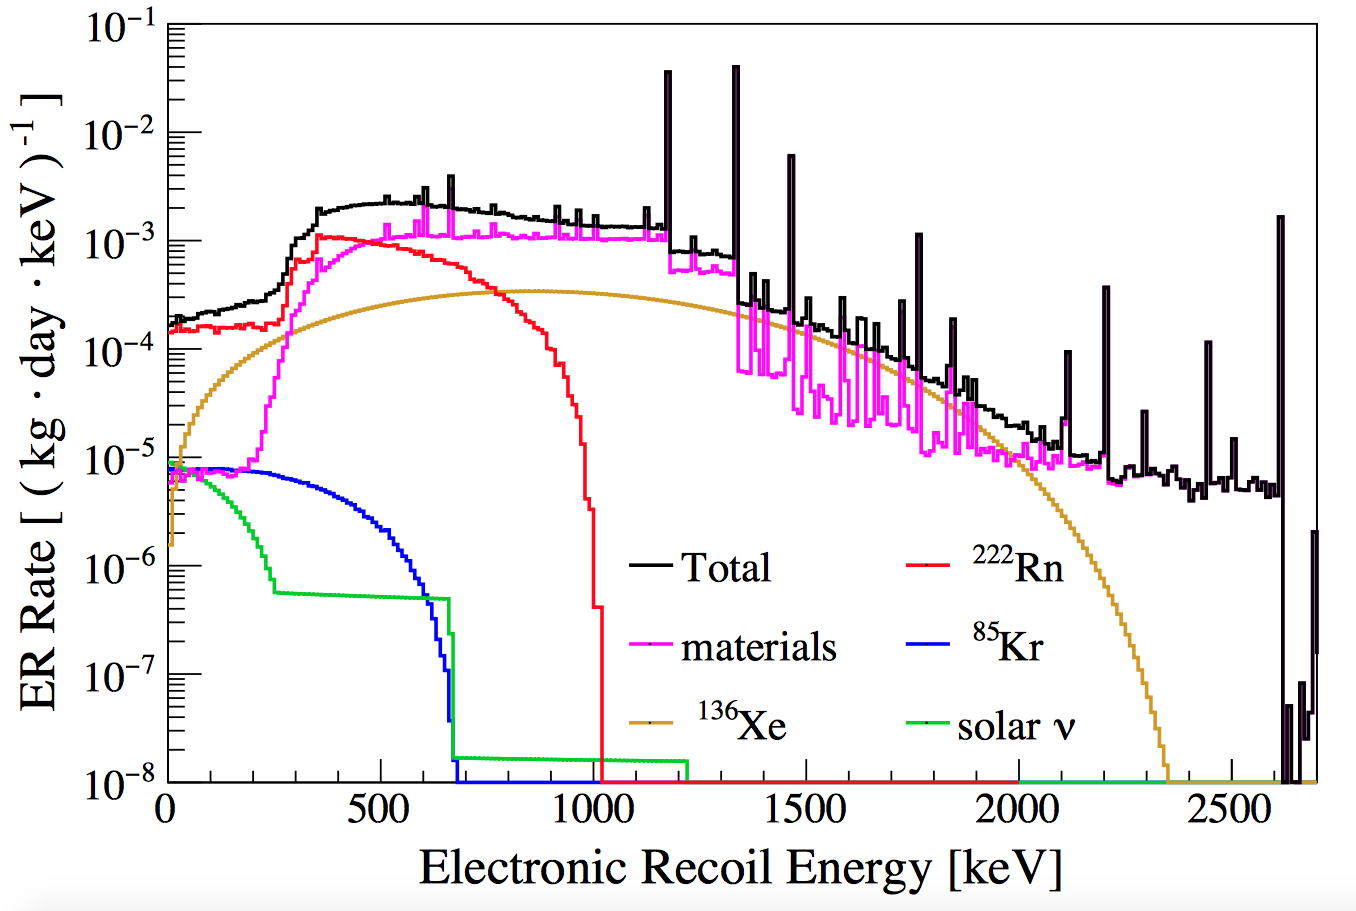
\includegraphics[height=5cm]{ERRateMCFull}
    \end{subfigure}%
    \begin{subfigure}[t]{0.5\textwidth}
        \centering
        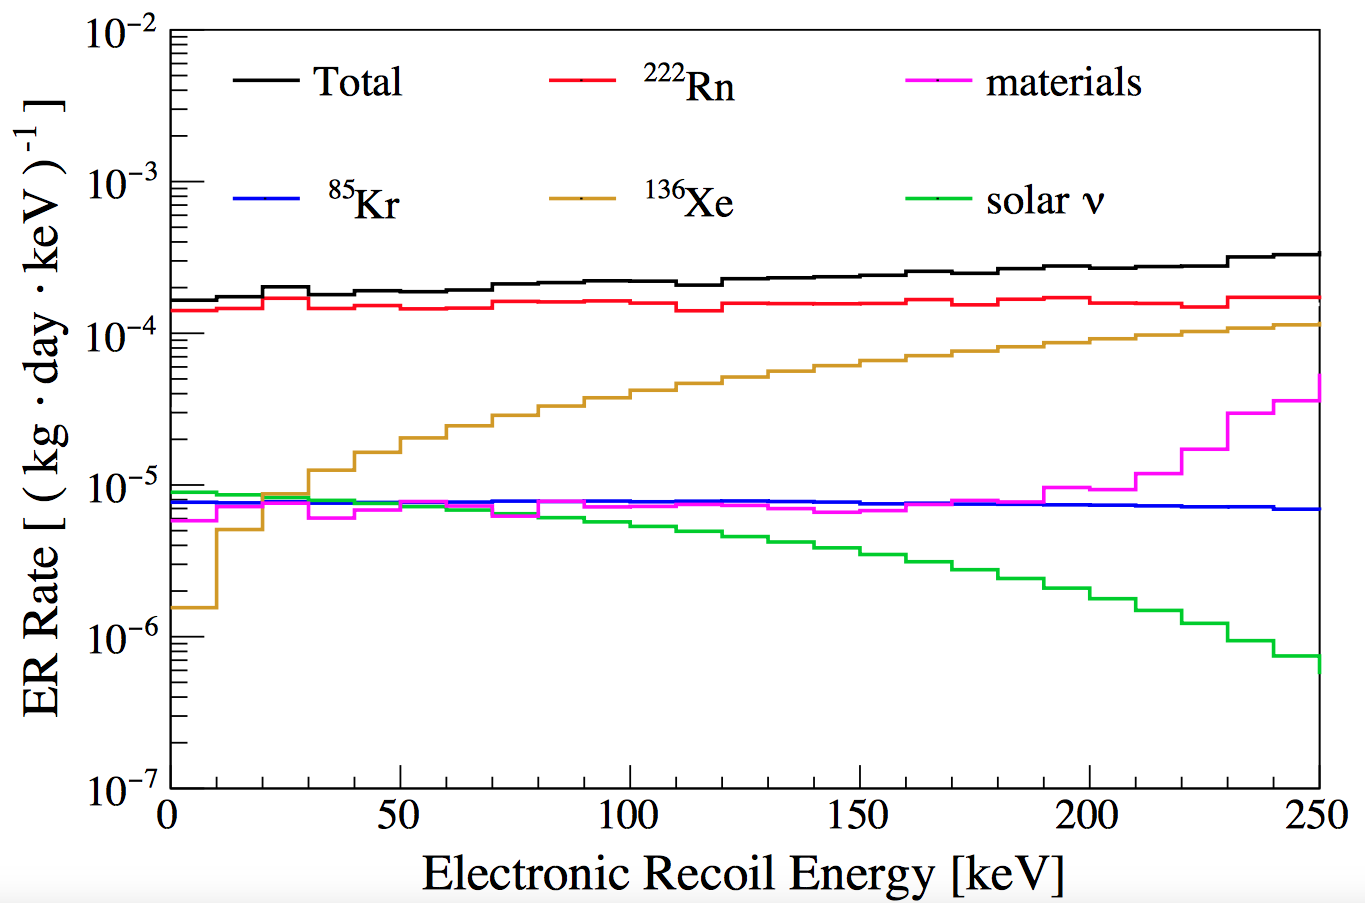
\includegraphics[height=5cm]{ERRateMCZoomed}
    \end{subfigure}
    \caption{Electronic recoil energy spectrum in a 1 t fiducial volume from MC simulations.  Image credit: \citeref{Aprile2016a}.}
	\label{fig:backgrounds_er_spectrum}
\end{figure}



\subsubsection{\ce{^{136}Xe}}
\label{subsubsec:backgrounds_electronic_xe}
\ce{^{136}Xe} is the only unstable isotope of natural xenon.  It undergoes $2 \nu \beta^- \beta^-$ decay with
$t_{1/2} = 2.17 \times 10^{21}\ \mathrm{years}$ (\citeref{Albert2014}) and a Q-value of 2458 keV.  Because of its abundance in natural
xenon (\ce{^{136}Xe}/\ce{Xe} = 8.9\%) its presence is unavoidable.  At the scale of XENON1T it is subdominant - only responsible for
${\sim}2 \%$ of the total ER background, as seen in \figref{fig:backgrounds_er_spectrum} (right).  However, as detectors continue to grow
it will become much more consequential.



\subsubsection{Solar Neutrinos}
\label{subsubsec:backgrounds_electronic_solar_neutrinos}
Solar neutrinos can elastically scatter off electrons, causing low-energy electronic recoils.  The recoil spectrum is the green line in
\figref{fig:backgrounds_er_spectrum}.  As with the \ce{^{136}Xe} $2 \nu \beta^- \beta^-$
decay its contribution is small, but as an irreducible background it will become more problematic as detectors grow.



\subsection{Nuclear Recoils}
\label{subsec:backgrounds_nuclear}
Our nuclear recoil background comes from neutrons and neutrinos.  Whereas \gammarays are stopped within several cm, high-energy neutrons
have mean free paths of $\mathcal{O}(10)$ cm, allowing them to move through the LXe volume more easily and giving a higher probability
that it scatters once inside the FV.  Neutrinos move freely and cannot be shielded.  The nuclear recoil background is composed of
radiogenic and muon-induced neutrons as well as from astrophysical neutrinos.



\subsubsection{Radiogenic Neutrons}
\label{subsubsec:backgrounds_nuclear_radiogenic}
Radiogenic neutrons are produced by primordial decay chains \ce{^{238}U}, \ce{^{235}U} and \ce{^{232}Th} in detector materials
(see \secref{subsec:backgrounds_detector_materials} for discussion on electronic and $\alpha$ recoils).  They are released in
$(\alpha, \mathrm{n})$ reactions that result from the $\alpha$-emissions along the decay chains, as well as spontaneous fission (SF).  For
heavier nuclei radiogenic neutrons are generated almost exclusively by SF as the $(\alpha, \mathrm{n})$ reaction is suppressed by the
large Coulomb barrier (\citeref{Aprile2016a}).

\figref{fig:backgrounds_nuclear_radiogenic_rates} shows the neutron yield as a function of energy for PTFE and copper from Monte Carlo
predictions.  The chains are
separated to $\mathrm{^{238}U} \rightarrow \mathrm{^{230}Th}$ and $\mathrm{^{226}Ra} \rightarrow \mathrm{^{206}Pb}$, and
$\mathrm{^{232}Th} \rightarrow \mathrm{^{228}Ac}$ and $\mathrm{^{228}Th} \rightarrow \mathrm{^{208}Pb}$ to account for the disequilibrium
that was observed.  The PTFE has on average a lighter $Z$ than the copper, giving it a larger $(\alpha, \mathrm{n})$ contribution (dashed
lines represent SF-only).  We can see in \figref{fig:backgrounds_nuclear_muon_induced_nr_rate} that for $E \gtrsim 3\ \mathrm{keV}$
radiogenic neutrons are the dominating factor for the NR backgrounds.  The expected rate for 1 ton is
$0.6 \pm 0.1\ \mathrm{y^{-1}}$.

\begin{figure}
    \centering
    \begin{subfigure}[t]{0.5\textwidth}
        \centering
        \includegraphics[height=5cm]{neutronyield-ptfe-v2}
    \end{subfigure}%
    \begin{subfigure}[t]{0.5\textwidth}
        \centering
        \includegraphics[height=5cm]{neutronyield-cu-v2}
    \end{subfigure}
    \caption{Image credit:Image credit: \citeref{Aprile2016a}.}
	\label{fig:backgrounds_nuclear_radiogenic_rates}
\end{figure}



\subsubsection{Muon Induced Neutrons}
\label{subsubsec:backgrounds_nuclear_muon_induced}
Cosmic muons interacting with the rock above the detector can produce up to GeV neutrons.  The large mean free path from such high energy
makes it not unlikely that they pass through the water shield (\secref{subsec:xenon1t_water_shield}).  However, simulations show that if
the associated showers from the muon interaction also enter the tank the tagging efficiency is $> 70\%$.  Still the predicted rate is just
$< 0.01\ \mathrm{y^{-1}}$ for 1 t and is represented by the blue line in \figref{fig:backgrounds_nuclear_muon_induced_nr_rate}.

\begin{figure}
\centering
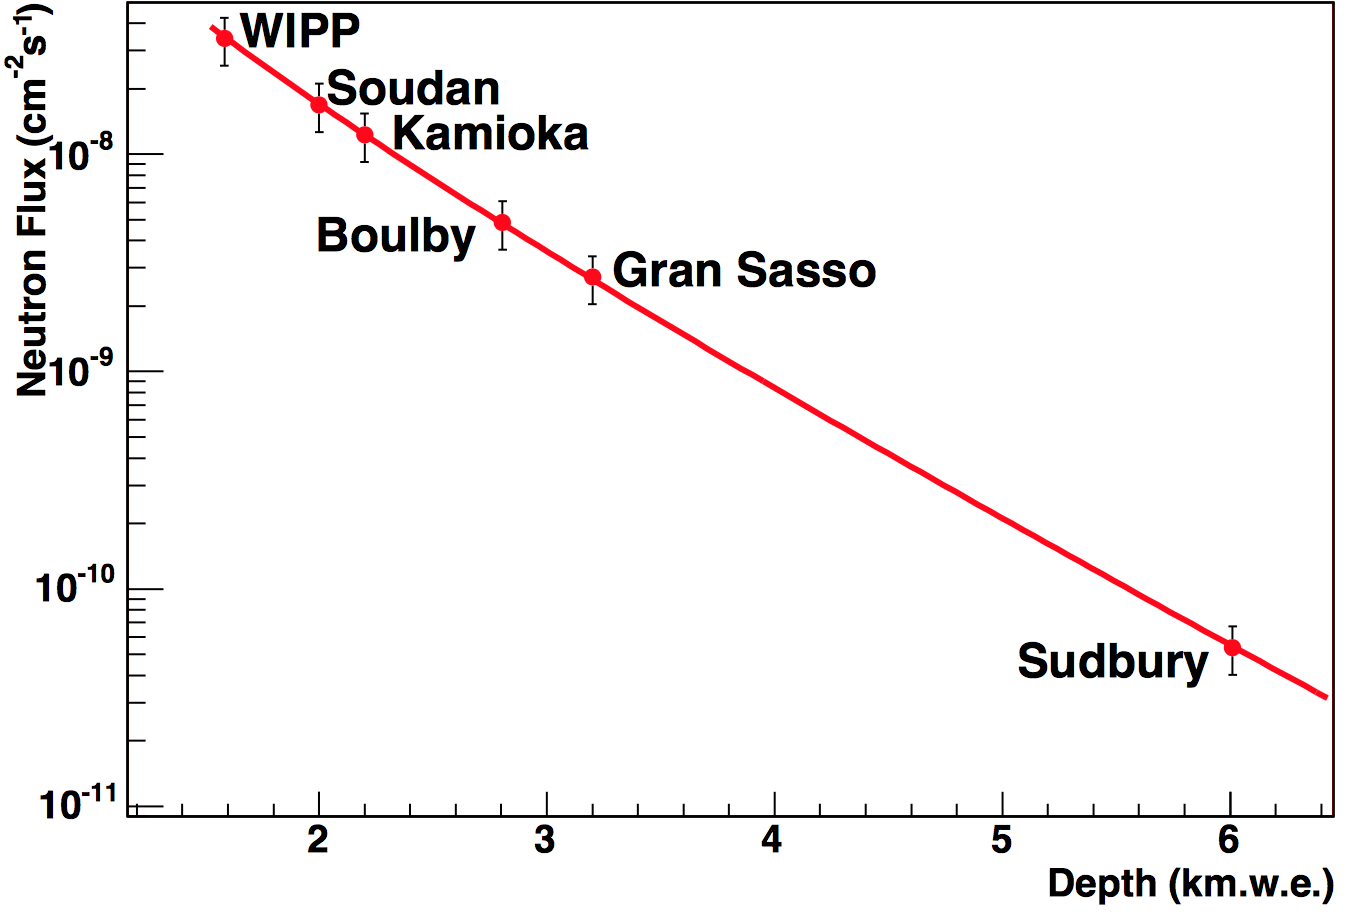
\includegraphics[width=0.6\textwidth]{MuonFluxOverDepth}
\label{fig:backgrounds_nuclear_muon_induced_flux}
\end{figure}

\begin{figure}
\centering
\includegraphics[width=0.6\textwidth]{totalnrbackground}
\caption{Image credit: \citeref{Aprile2016a}.}
\label{fig:backgrounds_nuclear_muon_induced_nr_rate}
\end{figure}



\subsubsection{Neutrinos}
\label{subsubsec:backgrounds_nuclear_neutrinos}
The final contribution to the NR background comes from neutrinos that participate in coherent neutrino-nucleus scattering.  The primary
contributor to the integrated NR rate is solar \ce{^{8}B}, which is orders of magnitude larger than other sources and dominant at
recoil energies $< 3\ \mathrm{keV}$.  Solar $hep$, atmosphere, and diffuse supernova neutrinos also contribute.  We can see in
\figref{fig:backgrounds_nuclear_muon_induced_nr_rate} that neutrinos are the principal source for recoils at $< 3\ \mathrm{keV}$.  The
number of detected events at $> 1\ \mathrm{keV}$ was predicted to be ${\sim} 90\ \mathrm{t^{-1}\ y^{-1}}$.  While this is below our
threshold, Poissonian variations may put a small fraction into our detection region.  By looking at the expected number of events closer
to our threshold (${\sim} 4\ \mathrm{keV}$) this drops to $1.8 \times 10^{-2}\ \mathrm{t^{-1}\ y^{-1}}$.  As mentioned in
\secref{subsubsec:backgrounds_electronic_solar_neutrinos} neutrinos will compose a greater fraction of our background due to the inability
to shield them.



\subsection{Detector Materials}
\label{subsec:backgrounds_detector_materials}
As mentioned in \secref{subsec:xenon1t_pmts} and \secref{subsec:xenon1t_cryo} detector materials were screened before purchasing to ensure
those with the lowest radioactivity were chosen.  The high self-shielding power of LXe prevents the radiation from penetrating far into
the detector, stopping the majority within several cm.  Still, it is important to understand our background for a number of reasons.  The
first is we want to maximize our FV.  But because including these events can have a negative effect on our sensitivity, we need to know
what a safe distance from the top, bottom, and wall are.  The second is once we choose our FV it is important to have a reliable estimate
of the number of events that will ``leak" into our FV, known as ``leakage events".  Failing to have an accurate prediction can result in
a cost in sensitivity.  A third reason is these events can play a significant role in characterizing the detector.

The primary isotopes from materials that play a role in our background are \ce{^{40}K}, \ce{^{60}Co}, \ce{^{235}U}, and the decay chains
of and \ce{^{238}U}, \ce{^{232}Th}, \ce{^{228}Th}, and \ce{^{226}Ra}.  In fact, although \ce{^{226}Ra} and \ce{^{228}Th} are part of the
\ce{^{238}U} and \ce{^{232}Th} chains, respectively, the measured disequilibrium prompts us to separate them as
$\mathrm{^{238}U} \rightarrow \mathrm{^{230}Th}$ and $\mathrm{^{226}Ra} \rightarrow \mathrm{^{206}Pb}$ for \ce{^{238}U}, and
$\mathrm{^{232}Th} \rightarrow \mathrm{^{228}Ac}$ and $\mathrm{^{228}Th} \rightarrow \mathrm{^{208}Pb}$ for \ce{^{232}Th}.  The full
\ce{^{238}U} and \ce{^{232}Th} chains can be seen in \figref{fig:backgrounds_decay_chains}.

\begin{figure}
    \centering
    \begin{subfigure}[t]{0.5\textwidth}
        \centering
        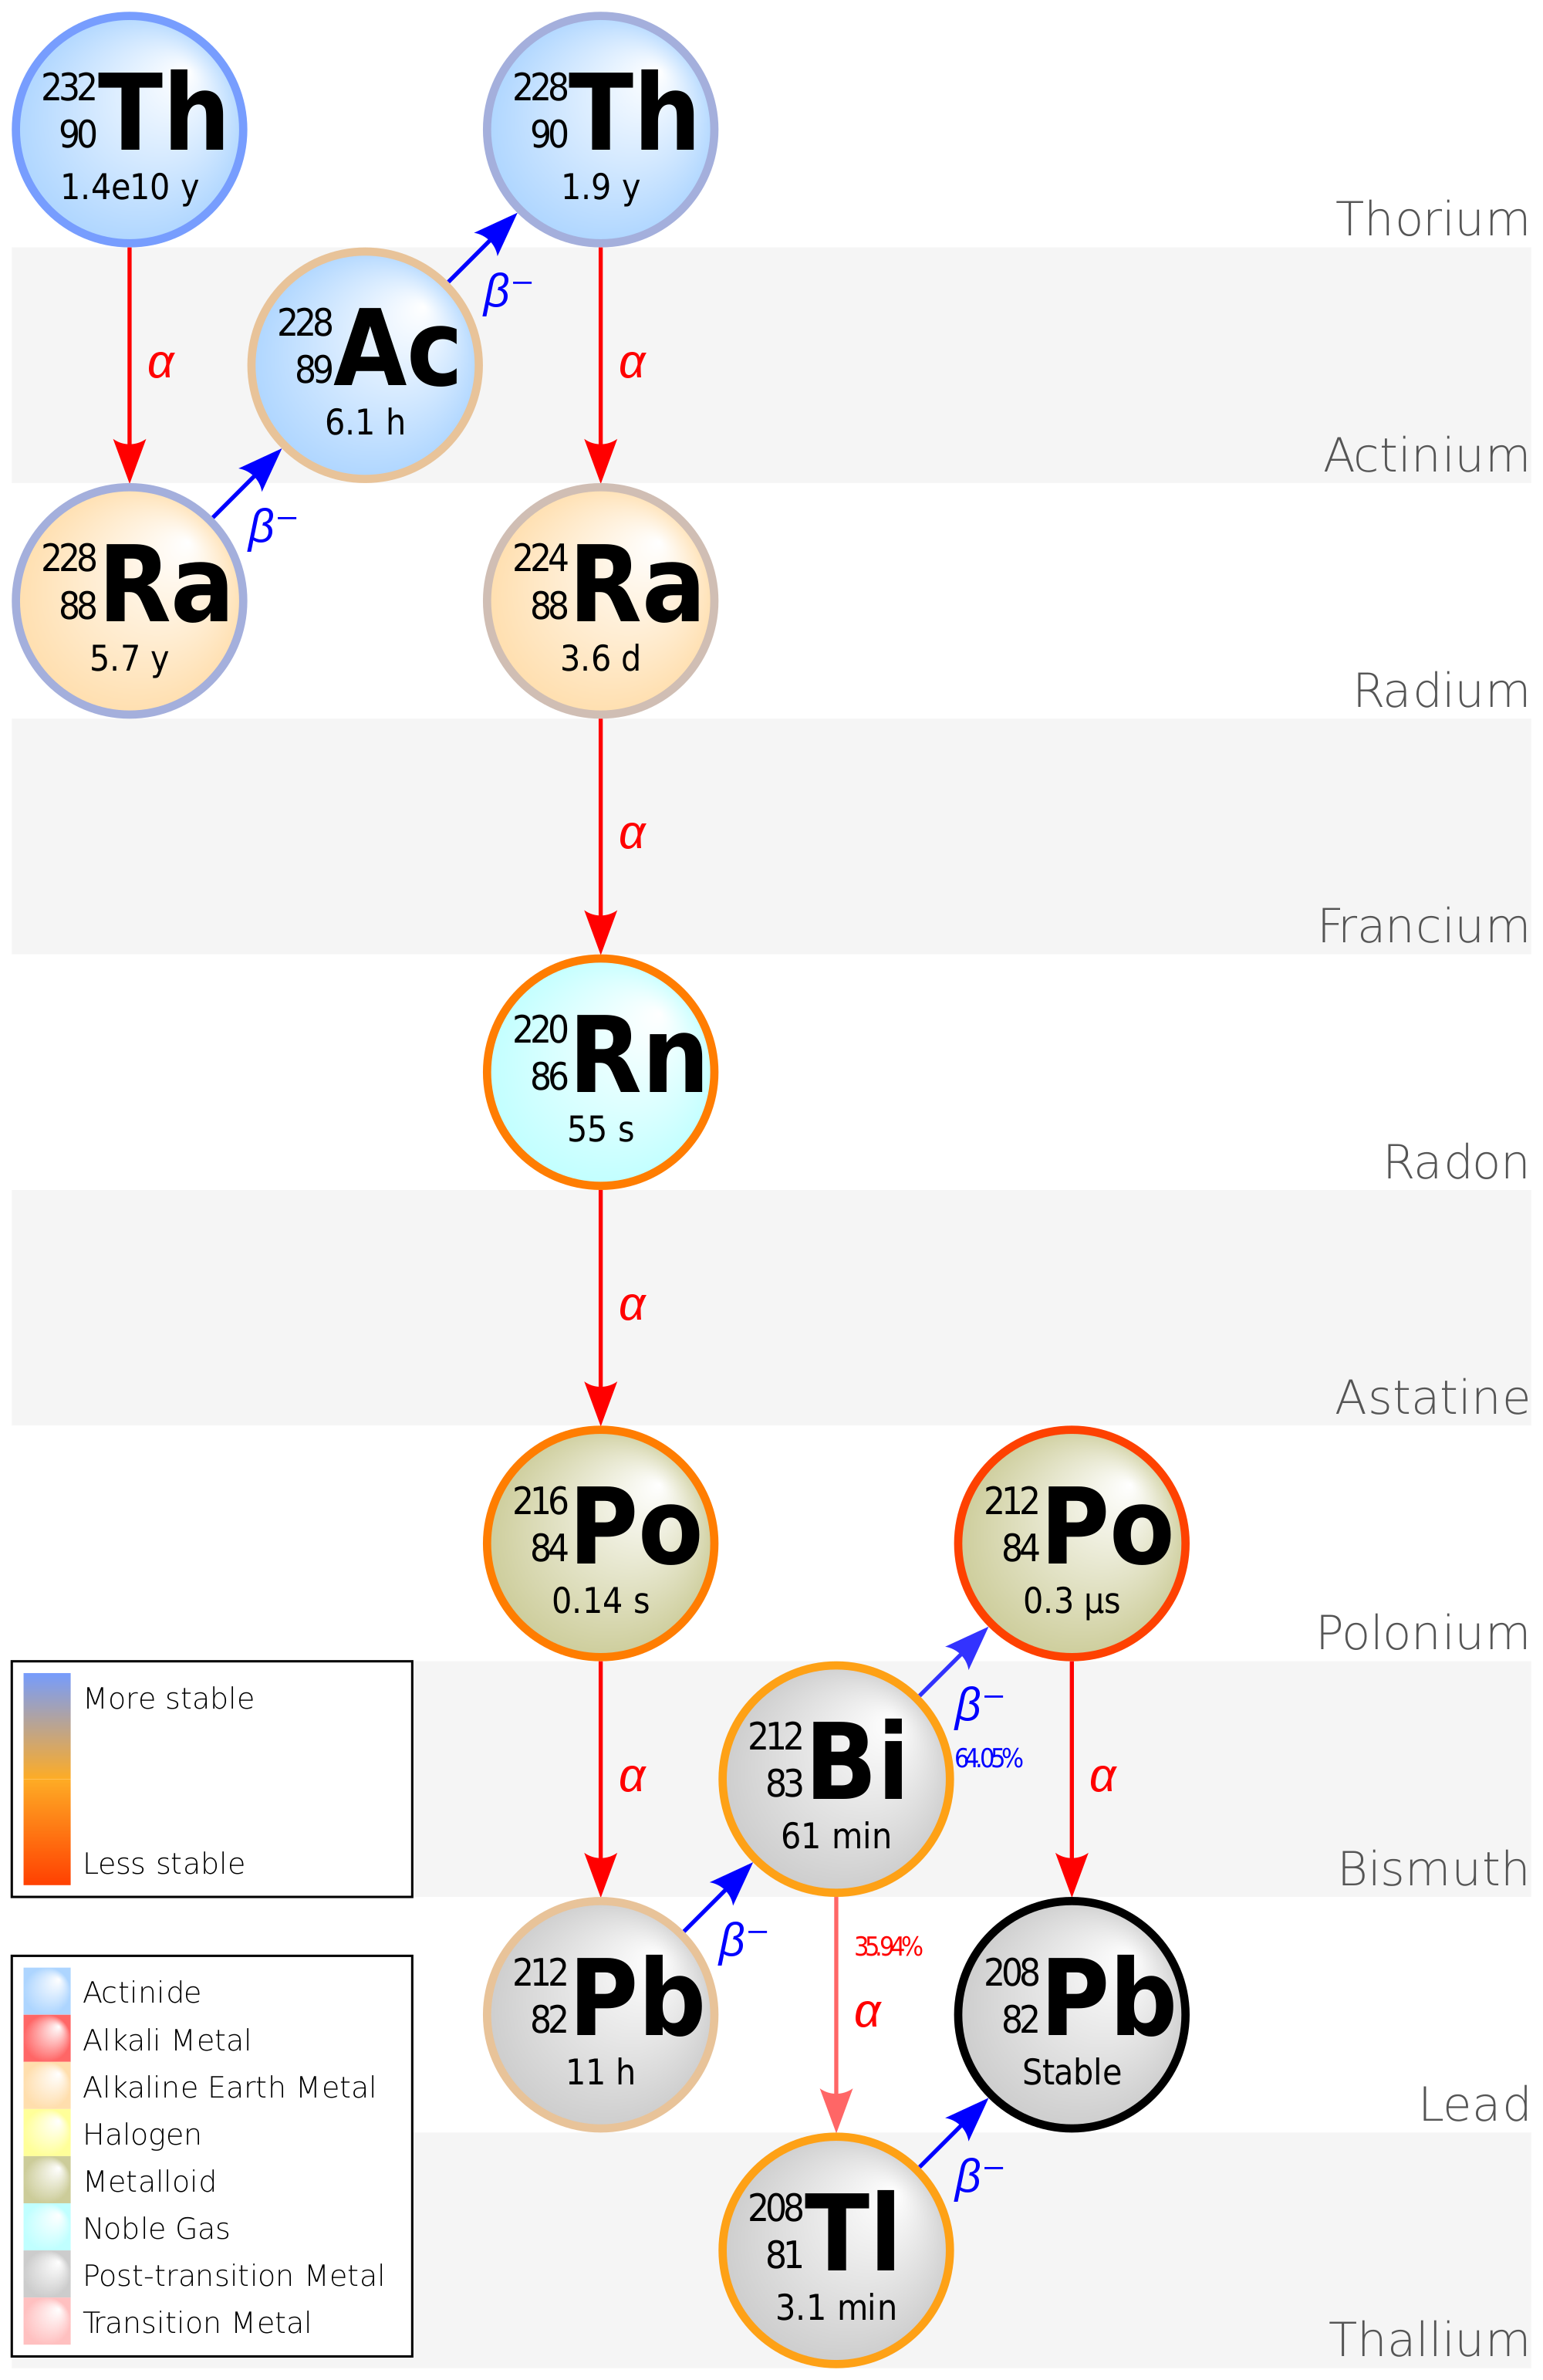
\includegraphics[width=\textwidth]{Decay_Chain_of_Thorium-232}
    \end{subfigure}%
    \begin{subfigure}[t]{0.5\textwidth}
        \centering
        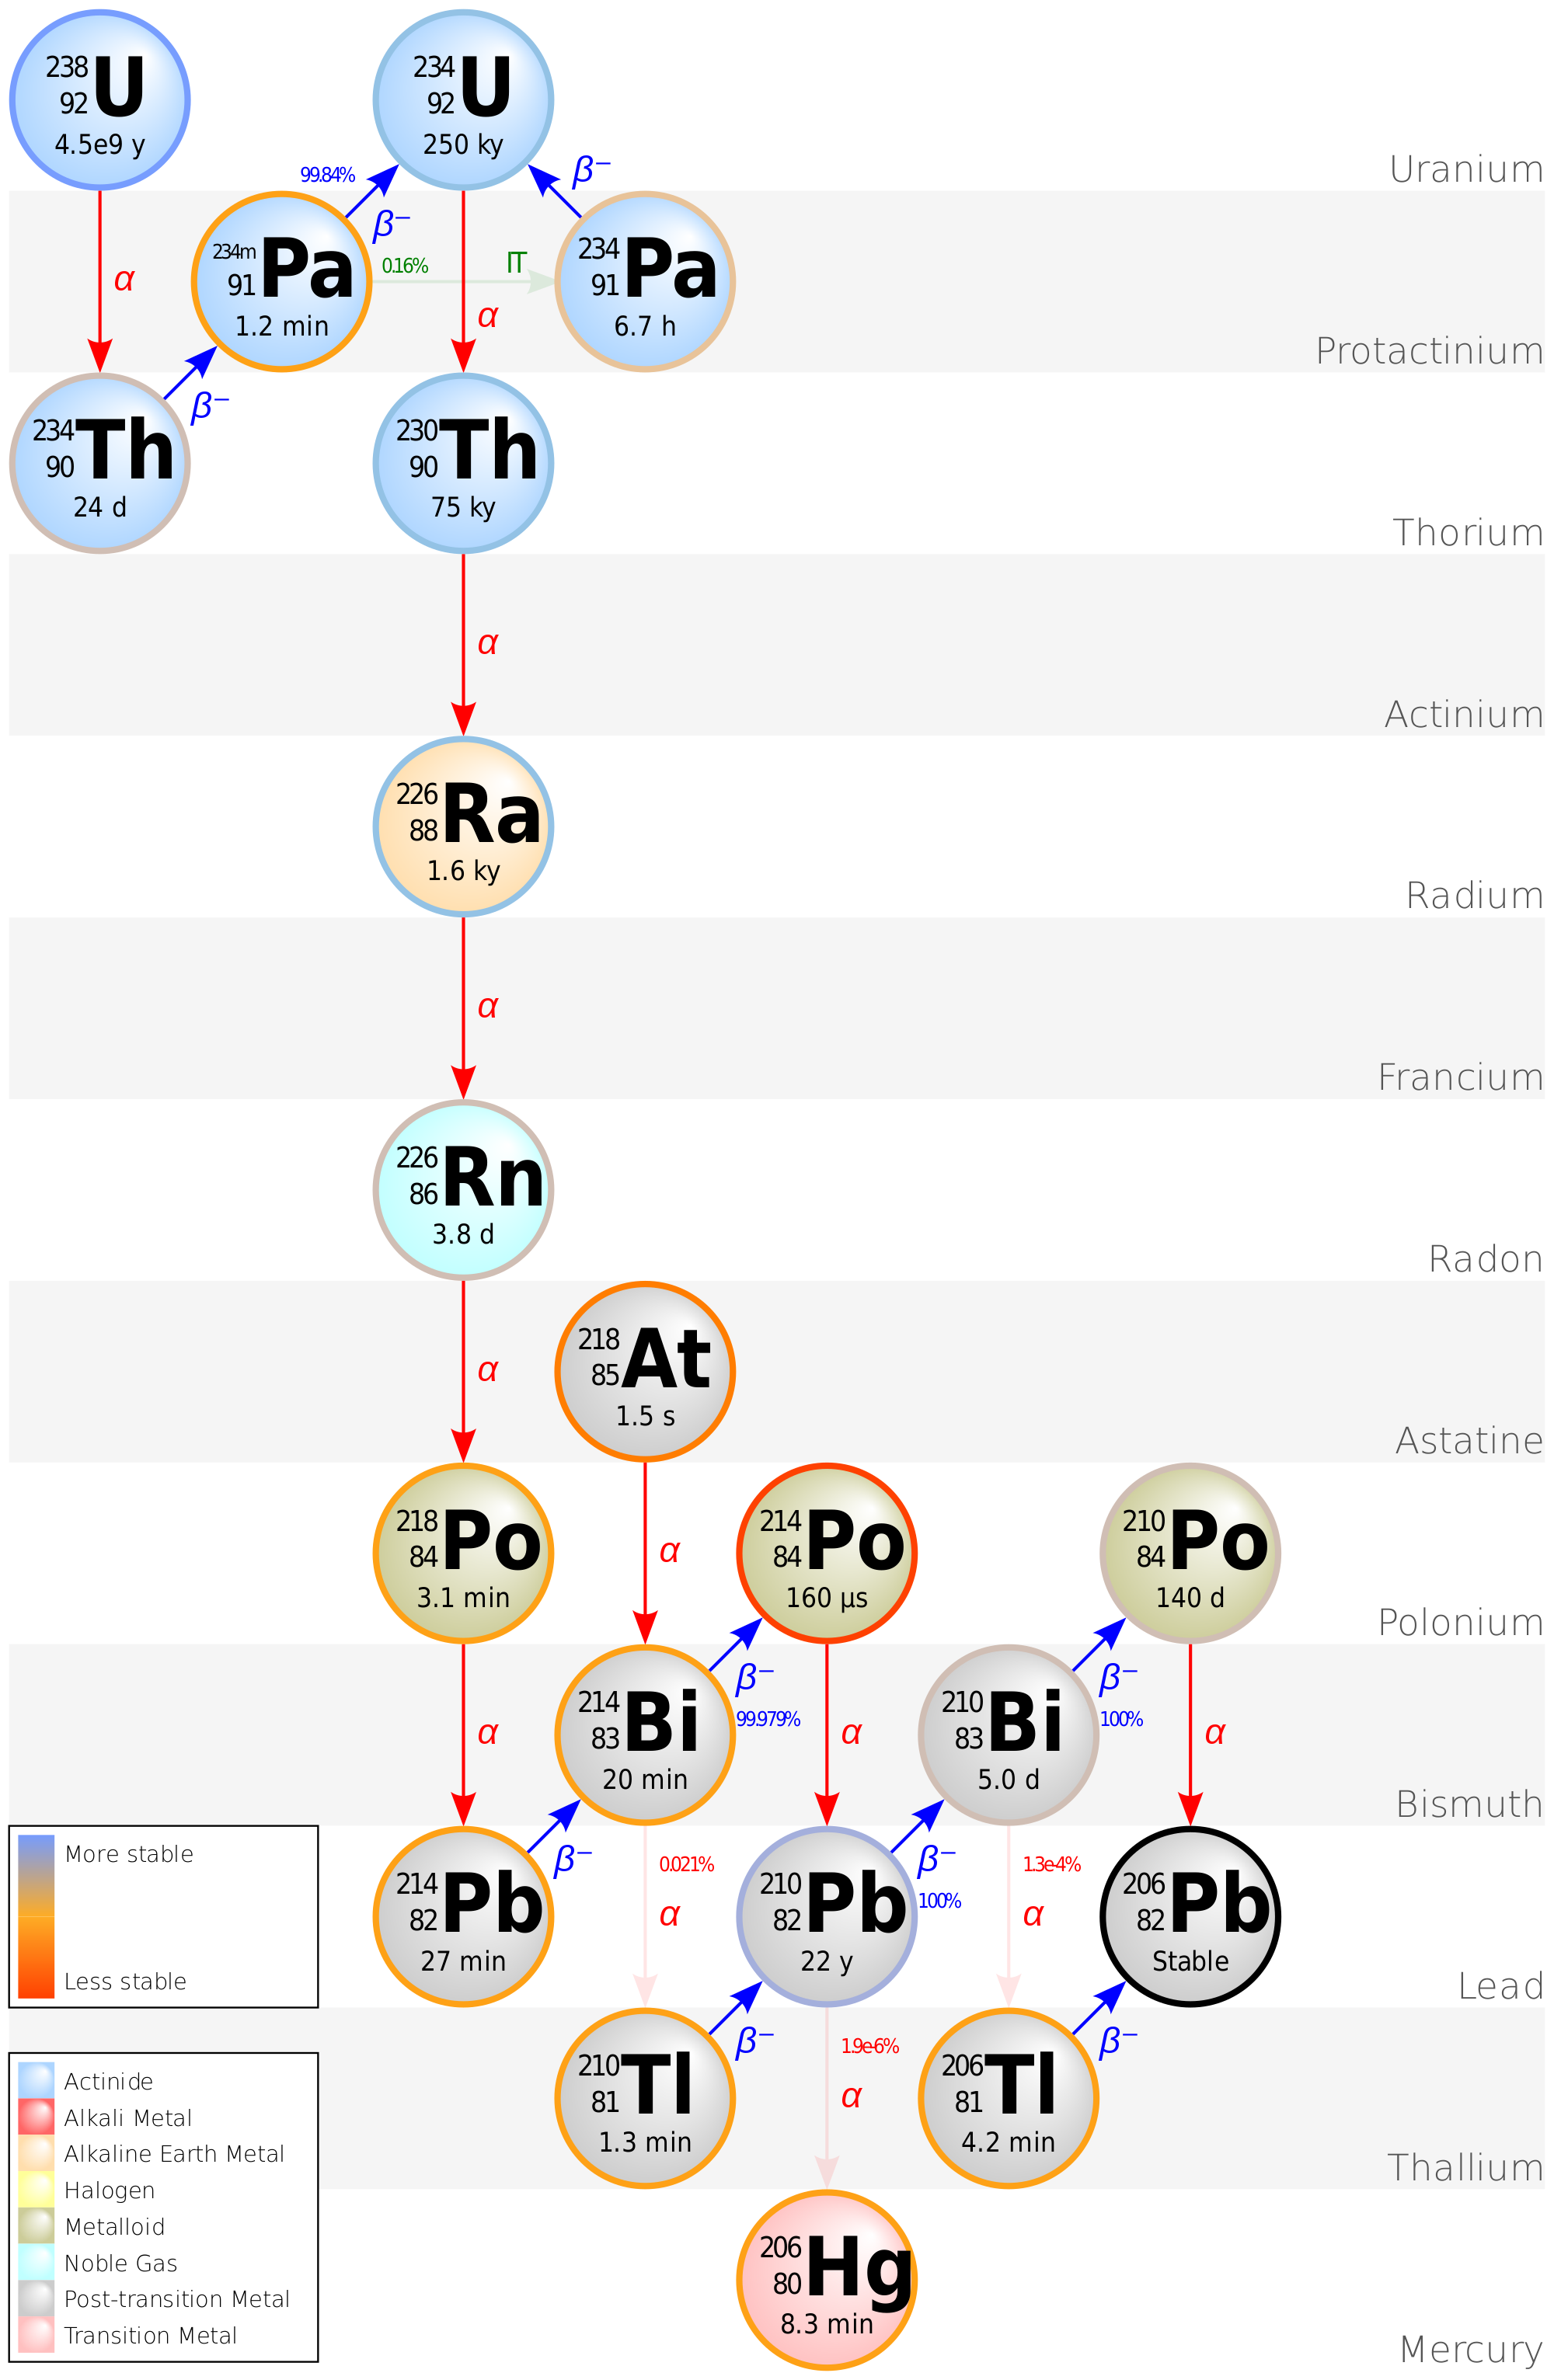
\includegraphics[width=\textwidth]{Decay_Chain_of_Uranium-238}
    \end{subfigure}
    \caption{Decay chains for \ce{^{232}Th} (left) and \ce{^{238}U} (right).  Image credit: \citeref{Wikimedia2018a, Wikimedia2018b}.}
	\label{fig:backgrounds_decay_chains}
\end{figure}

As \electron from wall events drift to the surface a fraction will attach to the PTFE.  This decrease in S2 causes three main effects: 1)
an increase in position reconstruction uncertainty, 2) electronic recoil events to leak into the NR band, and 3) producing small changes
to the electric field.

A major constraint on the radius of our fiducial volume is the radioactivity from the PTFE panels - both the rate and reconstructed
positions, the latter of which has significant uncertainty at $\mathrm{S2_b} \lesssim 1000\ \mathrm{PE}$
(\figref{fig:calibrations_position_reconstruction_res}).  This makes \ce{^{210}Pb} on the PTFE panels concerning since its \betadecay has
a Q-value of just $63.5\ \mathrm{keV}$ and electron loss could result in a seemingly normal NR event inside our FV.  Moreover, despite a
chemical cleaning process during commissioning, a large amount of \ce{^{210}Pb} is known to be present from observations of its progeny
\ce{^{210}Po} $\alpha$-decays.  With a half-life of $t_{1/2} = 22.1\ \mathrm{y}$ and the continual addition of \ce{^{222}Rn}
(\secref{subsubsec:backgrounds_electronic_radon}), which quickly decays to \ce{^{210}Pb} within days, the background rate will be
constant over the lifetime of the detector.

To adress the first two points we model our expected contamination with events whose positions were reconstructed outside the
TPC ($r > 47.9\ \mathrm{cm}$).  The S2, cS1, cS2$_{\mathrm{b}}$, and $z$
distributions were found to be symmetric inside and outside the TPC, which was expected since the S2 was detected at the boundary.  The
$r > 47.9\ \mathrm{rm}$ data was unblinded and the energy distribution was obtained via a fixed kernel density (KDE) estimator using
superposition of gaussians for each point in S2, cS1, cS2$_{\mathrm{b}}$, and $z$ space.

Three complementary S2$_{\mathrm{b}} - r$ PDFs were
constructed using a skew gaussian ($M1$), skew t ($M2$), and adaptive KDE ($M3$).  The minimum, average, and maximum PDF methods were determined
by $\mathrm{min}(M1, M2, M3)$, $\mathrm{mean}(M1, M2, M3)$, and $\mathrm{max}(M1, M2, M3)$, respectively.  These were unified with the
KDE for a 5D predictor of the event distribution inside the TPC.

\begin{figure}
    \centering
    \begin{subfigure}[t]{0.5\textwidth}
        \centering
        \includegraphics[width=\textwidth]{WallS2S1}
    \end{subfigure}%
    \begin{subfigure}[t]{0.5\textwidth}
        \centering
        \includegraphics[width=\textwidth]{WallS2R}
    \end{subfigure}
    \caption{\cstwob vs. cS1 distribution for background wall leakage events outside the TPC ($r > 47.9\ \mathrm{cm}$) is shown on the
    left.  The events overlap with the ER (color) and NR (color) bands, the latter of which might appear as a WIMP.  On the right is
    the S2 vs. $r$ distribution.  Data outside and inside the TPC appear symmetric in $r$.  The effects of poor position reconstruction
    at low S2 is observed.}
	\label{fig:backgrounds_decay_chains}
\end{figure}

\begin{figure}
\centering
\includegraphics[width=0.8\textwidth]{surface_s2s1_distribution_blessed_sr1}
\caption{Expected surface background distribution in cS1-cS2$_{\mathrm{b}}$.  Electrons from wall events attach to the PTFE as they drift,
decreasing the S2 and moving towards the NR band.  Projections are
shown for cS1 (top) and cS2$_{\mathrm{b}}$ (right) for all events in blue, and between the NR median (red dashed line) and
$-2 \sigma$ (black) in orange.  We can see the surface background has the largest impact in our ROI at
$\mathrm{cS2_{\mathrm{b}}} \lesssim 400\ \mathrm{PE}$, $\mathrm{cS1} \lesssim 20\ \mathrm{PE}$.}
\label{fig:backgrounds_detector_materials_bands}
\end{figure}

The accumulation of charge on the PTFE panels was discovered by the author by tracking the number of \ce{^{222}Rn} and \ce{^{218}Po}
$\alpha$-decays.  By monitoring the total number of events in the TPC the rate was unchanging over time.  However, by imposing some radial
cut it was discovered that the rate was increasing as \electron were pushed away from the walls, as seen in
\figref{fig:backgrounds_wall_charge}.  This meant that our FV was growing over the course of the lifetime of the experiment and we would
underestimate our background.  To account for this we recalculated the position reconstruction for each $\mathrm{^{83m}Kr}$
calibration and included a time dependent correction for analyses.

\begin{figure}
\centering
\includegraphics[width=\textwidth]{WallChargingPlot}
\label{fig:backgrounds_wall_charge}
\end{figure}

At $E \gtrsim 500\ \mathrm{keV}$ the background contribution becomes dominated by detector materials, except for
${\sim} 1400 \mdash 2100\ \mathrm{keV}$ where \ce{^{136}Xe} is slightly larger.  For the energy region for spin-independent WIMP dark matter
though it is outpaced by more than an order of magnitude inside a 1 t FV.  \figref{fig:backgrounds_er_spectrum} shows the predicted ER
backgrounds using Monte Carlo.



\subsection{Accidental Coincidence}
\label{subsec:backgrounds_ac}
In some circumstances we may not be able to observe both the S1 and S2.  Interactions with only an S1, or lone-S1 events, result almost
entirely from PMT dark rate pile-up at low energies, and below-cathode scatters at higher.  Those with just an S2, or lone-S2 events,
come from interactions near the cathode and gate where the large electric field can significantly quench the S1.  The lone-S2s
could at least in part be explained by \ce{^{210}Pb}, which given its presence on the PTFE panels, suggest it may also exist on the
electrodes.

Generally lone-S1 and lone-S2 events do impact our data, but occasionally if they occur close to one another can mimic a real event, known
as accidental coincidence (AC).  Because we cannot know which events are AC, those that pass our cuts 
(\secref{subsubsec:er_nr_calibrations_parameter_determ_cuts}) will end up in our final data
selection.  A shape cut is applied to S1s to ensure it is not an S2 from a single electron.  It is therefore important to calculate the
number of expected events and the distribution.  The rate of AC events is given by

\begin{equation}
R_{\mathrm{AC}} = R_{\mathrm{LS1}} \times R_{\mathrm{LS2}} \times t_{d, \mathrm{max}}
\label{eq:er_nr_calibrations_parameter_determ_additional_components_accidental_coincidence}
\end{equation}

\noindent where $R_{\mathrm{LS1}}$ and $R_{\mathrm{LS2}}$ are the lone-S1
and -S2 rates and $t_{d, \mathrm{max}}$ is the maximum TPC drift time.  S1s, especially at low energy, are too small trigger the
DAQ.  Therefore, to calculate $R_{\mathrm{LS1}}$ we select higher energy good events that contain and S1 and S2, and search the region
before the primary S1.  This method makes two assumptions.  The first is that lone-S1s should be uncorrelated in time, and thus
distributed uniformly over large timescales.  The second is that the S1s we find do not have a complementary S2.  For the former this
seems reasonable since we do not expect PMT dark rates and below-cathode scatters to follow any pattern.  The latter is valid because
the probability of having two interactions in the same time window is negligible.

\begin{figure}
\centering
\includegraphics[width=0.8\textwidth]{ac_s2s1_distribution_blessed_sr1}
\caption{Expected accidental coincidence distribution in cS1-cS2$_{\mathrm{b}}$ space.  Isolated S1s and S2s are randomly coupled to
imitate real events in the TPC.  S1 and S2 corrections are applied and events that pass the cuts are plotted.  Projections are
shown for cS1 (top) and cS2$_{\mathrm{b}}$ (right) for all events in blue, and between the NR median (red dashed line) and
$-2 \sigma$ (black) in orange.}
\label{fig:er_nr_calibrations_parameter_determ_ac}
\end{figure}

Accidental coincidence does not benefit from fiducialization like much of our other background.  In fact, we can see from
\eqnref{eq:er_nr_calibrations_parameter_determ_additional_components_accidental_coincidence} that $R_{\mathrm{ac}}$ actually increases
with detector size.  Still, its total contribution is comparatively small.  AC is source or background-dependent, so for this analysis
distributions for \ce{^{220}Rn}, $\mathrm{^{241}AmBe}$, and the NG each were included in the
fit.  Similar conditions and duration meant the SR0 and SR1 $^{241}$AmBe calibrations had nearly the same AC expectation so it was not
necessary to include independent distributions; however, SR0 and SR1 AC \ce{^{220}Rn} were sufficiently different this could not be
done for ER.  \figref{fig:er_nr_calibrations_parameter_determ_ac} shows the expected AC distribution in (cS1, cS2$_{\mathrm{b}}$) space
with the region of interest shown in dotted red (median) and black ($-2 \sigma$) lines.




\section{Electronic and Nuclear Recoil Bands}
\label{sec:er_nr_calibrations}
To differentiate our nuclear from electronic recoil bands we need to calibrate each independently.  While the detector characterizations
discussed in \secref{sec:det_char} lead to improved accuracy and precision or are in some cases very important, these are critical as
they allow discrimination between at potential WIMP and ER background.  As mentioned in
\secref{subsec:det_char_elifetime} \ce{^{220}Rn} is used for our ER band.  For NR we use \ce{^{241}AmBe} and a deuterium-deuterium
neutron generator (NG), both of which are positioned in the water tank outside the cryostat.

Fitting the bands for this analysis was unique in that it fit all five calibrations from both science runs simultaneously.  This was
significant because it forced values that are common to some or all of the calibrations (e.g. $W$, $p_{\mathrm{dpe}}$, etc. are shared
between all five, while $g_1$, $g_{2\mathrm{b}}$, etc. are shared within each science run) to converge to a single value.\footnote{for First Results
the \radoncal and \ambe were independently fit.}  \tabref{tab:er_nr_calibrations_parameters} lists the variables included in the fit and
to which calibrations they apply.



Using the physical processes from the interaction itself to the final values of cS1 and \cstwob in the fit is made
possible by running on GPUs, which provide a $10^{2 \mdash 3}$ times speed increase.



\subsection{Purpose of Calibrations}
\label{subsec:er_nr_calibrations_purpose}
The electronic and nuclear recoil calibrations are important because they create a probability density function (PDF)
such that for any event we can quantify the likelihood of what caused it.  This provides dramatically improved sensitivity
to purely statistical approaches (\secref{sec:direct_detect}).  Doing so requires a complete understanding of the TPC background, which
in addition to nominal electronic recoils includes accidental coincidence (AC) and wall leakage events
\secref{subsubsec:er_nr_calibrations_parameter_determ_additional_components}.  It also demands that
the physical processes that occur starting from the exciton-ion ratio through the data acquisition are correctly modeled and able to be
simulated on a reasonable time scale.

Following the ER and NR fits a signal PDF is generated.  For our DM search the
signal is a WIMP but in general it is not constrained to this.  The shape of the PDF depends on the WIMP mass.  The data can be compared
to the PDF for a given WIMP mass and cross-section to see whether it agrees with a signal.  A limit is set if all cross-sections below
some value match the data, while a discovery can be claimed if the data prefers a particular mass and cross-section over others.

\figref{fig:er_nr_calibrations_wimp_contours} shows the background model with contours for a 50 GeV WIMP overlaid.  The ER band is clearly
present and we can see the overlap between the two, which exemplifies the necessity of lowering the overall background for improved
sensitivity.

\begin{figure}
\centering
\includegraphics[width=\textwidth]{WIMPContours}
\caption{Some on SR0 blessed plots page}
\label{fig:er_nr_calibrations_wimp_contours}
\end{figure}



\subsection{Parameter Determination}
\label{subsec:er_nr_calibrations_parameter_determ}
This approach compares the distribution of Monte Carlo events with the data.  Because of the nearly flat distribution of events at relevant
energies along with homogenous distribution, Monte Carlo features $E_{\mathrm{true}}$, $x_{\mathrm{true}}$, $y_{\mathrm{true}}$,
$z_{\mathrm{true}}$, for \ce{^{220}Rn} are randomly sampled from a
uniform distribution.  \ce{^{241}AmBe} and neutron generator Monte Carlo are generated using GEANT4, and also include the number of
scatters for each neutron.  The $\beta^-$ from \ce{^{220}Rn} should not scatter so this is fixed to 1.  These values represent the ``truth''
information - that is, these are the true interaction values.  Reconstructed values will be referred to as $x_{\mathrm{rec}}$ and
$y_{\mathrm{rec}}$ (energy and depth will be denoted $E$ and $z$ and are equivalent in the fast-MC to the truth values).

\figref{fig:er_nr_calibrations_parameter_determ_flow_chart} shows the flow chart for the band matching.  Each Monte Carlo event is run
through a series of events that mimic the true sequence as closely as possible.  The parameters used in this estimation come from
a variety of sources including physical properties reported from literature and detector characterization measurements
(\secref{sec:det_char}).  The process takes the simulated energy from a Monte Carlo event and ultimately outputs observables cS1 and
$\mathrm{cS2_b}$.  These in turn are binned in cS1 vs. $\mathrm{log_{10}(cS2_b / cS1)}$ space, and the likelihood for equivalent bins
between data and MC is calculated (\secref{subsubsec:er_nr_calibrations_parameter_determ_mc_match}).  To describe our energy region of
interest as well as possible only events with $0 \leq \mathrm{cS1} \leq 100$ and $0.5 \leq \mathrm{log_{10}(cS2_b / cS1)} \leq 3.5$ are
considered.  As the parameters vary the likelihood should increase or decrease, allowing a minimizer to find the best-fit values.

\begin{figure}
\centering
\includegraphics[width=\textwidth]{FlowChart}
\label{fig:er_nr_calibrations_parameter_determ_flow_chart}
\end{figure}

The number of events simulated for each likelihood iteration is $\mathcal{O}(10^6)$.  Such large statistics are necessary for convergence;
however, nominal running time is far greater than any sensible time-scale.  This was solved by using graphical processing units (GPUs),
which can run the events in parallel, providing a boost in speed is $10^{2 \mdash 3}$ times and reducing the required time to a
reasonable level.

The conversion of truth MC to cS1 and \cstwob as a ``fast MC'' (the parameters used in each event are pulled
from a random number generator).  ``Truth MC'' will refer to the simulated events before the fast MC ($E_{\mathrm{true}}$,
$x_{\mathrm{true}}$, $y_{\mathrm{true}}$, $z_{\mathrm{true}}$, and number
of scatters as described above).  ``MC'' will denote the sum of all the fast MC components, usually in the form of a PDF (histogram), for
a single data-MC comparison.  Finally, a Markov Chain Monte Carlo (MCMC) is used to fit the data and Monte Carlo.  The best-fit values
then are derived from the posterior.  \secref{subsubsec:er_nr_calibrations_parameter_determ_er} (ER) and
\secref{subsubsec:er_nr_calibrations_parameter_determ_nr} (NR) discusses the physical steps that occur beginning with a single energy
deposition until final cS1 and $\mathrm{cS2_b}$ (and by extension the operations applied in the fast MC).

The calibrations were fit in the First Results FV ($-92.9 < z < -9\ \mathrm{cm}$, $r_{\mathrm{rec}} < 36.94\ \mathrm{cm}$
\figref{fig:calibrations_position_reconstruction}) despite it being different from the RC fiducial volume.  This was done to minimize wall
events as well as contamination from materials at the top and bottom of the TPC (mainly PMTs).



\subsubsection{Electronic Recoils}
\label{subsubsec:er_nr_calibrations_parameter_determ_er}
The electronic recoil calibration is performed using \ce{^{220}Rn} (decay chain shown in the left panel of
\figref{fig:backgrounds_decay_chains}).  It is used because of the \ce{^{212}Pb} \betadecay with Q-value 569.9 keV and can be performed
as an internal calibration.  In the future we hope to use tritiated methane $\mathrm{C H_3 T}$, which undergoes \betadecay
with a maximum energy of 18.6 keV.  This would provide significantly more statistics in our energy region of interest in a short amount
of time.  However, as mentioned in \secref{subsubsec:xenon1t_calibrations_internal} $\mathrm{C H_3 T}$ has a half-life of 12.3 y and there
is concern that it may attach to the cryostat.  For this reason we instead use \ce{^{220}Rn}, for which six separate calibrations were
performed during Science Run 1.

When energy is deposited in the LXe a number of quanta will be produced.  For electronic recoils this follows the normal distribution

\begin{equation}
n_q \sim \mathrm{Norm} \bigg( \mu = \frac{E}{W},\ \sigma^2 = \frac{E F}{W} \bigg)
\label{eq:er_nr_calibrations_parameter_determ_er_quanta}
\end{equation}

\noindent where $F$ is the Fano Factor (\citeref{Fano1947}) introduced in \secref{sec:er}.  Its derivation and subsequent measurements
demonstrates
that fluctuations in $n_{\mathrm{q}}$ are smaller than a Poisson distribution, and is estimated to be $F = 0.059$ (\citeref{Doke1976}).  For the
fast MC $F$ is held fixed, although it should be noted that a later measurement found different best-fit values, though their result was
compatible with \citeref{Doke1976} when including uncertainty (\citeref{Seguinot1995}).  $W$, the average energy to produce a single
quanta, is constrained by a Gaussian with $\mu = 13.7,\ \sigma = 0.2\ \mathrm{eV}$ following the measurement of \citeref{Dahl2009}.

For ER any quenching is considered negligible so is not considered.  The quanta will be divided into excitons and electron-ion pairs
$n_q = n_{\mathrm{ex}} + n_{\mathrm{ion}}$ and will be divided according to a binomial distribution

\begin{equation}
n_{\mathrm{ion}} \sim \mathrm{Binom} \Bigg(n = n_{\mathrm{q}},\ p = \frac{1}{1 + \frac{n_{\mathrm{ex}}}{n_{\mathrm{ion}}}} \Bigg)
\label{eq:er_nr_calibrations_parameter_determ_er_nions}
\end{equation}

\noindent where $n_{\mathrm{ex}} / n_{\mathrm{ion}}$ is between $0.06 \mdash 0.2$ and expected to be independent of energy
(\citeref{NEST2011}).  Next we must consider the recombination fraction $r$ where some \electron will reattach to a \ce{Xe^+} to form
excitons and upon decay to their ground state emit photons.  $r$ depends on the field in the LXe and the interaction energy, and has
intrinsic fluctuations $\Delta r$ (\citeref{LUX2016, Aprile2018a}).  A truncated Gaussian is assumed

\begin{equation}
r \sim \mathrm{Norm} \Big( \mu = \langle r \rangle,\ \sigma^2 = (\Delta r)^2 \Big)
\end{equation}

\noindent where $0 \leq r \leq 1$ and is parameterized using a modified Thomas-Imel box model (\citeref{Thomas1987})

\begin{equation}
\langle r \rangle = \frac{1}{1 + e^{-(E - E_0) / E_1}}
\bigg( 1 - \frac{\mathrm{ln}(1 + n_{\mathrm{ion}} \varsigma / 4)}{n_{\mathrm{ion}} \varsigma / 4} \bigg)
,\ \ \varsigma = \gamma_{\mathrm{er}} e^{-E / \omega_{\mathrm{er}}} F_{\mathrm{E}}^{-\delta_{\mathrm{er}}}
\label{eq:er_nr_calibrations_parameter_determ_ti}
\end{equation}

\noindent for the fit.  Here $\varsigma$ has been adapted from \eqnref{eq:ti_recomb} to include a power law field-dependence to allow
simultaneous fitting of SR0 and SR1, and an exponential energy term to extend compatibility to high energy
(${\sim} 20\ \mathrm{keV_{ee}}$).  An energy-dependent Fermi-Dirac is used to suppress recombination at
$\lesssim 2\ \mathrm{keV_{ee}}$ for better alignment with data.  The parameters have no prior and are constrained to
$0 \leq \gamma_{\mathrm{er}} \leq 0.5$, $0 \leq E_0, E_1 < \infty$, and
$-\infty < \omega_{\mathrm{er}}, \delta_{\mathrm{er}} < \infty$.

Recombination fluctuations are modeled as $\Delta r = A(1 - e^{-E/B})$.  Both parameters are allowed
to vary freely (with no penalty term in likelihood) with $A,B > 0$.  The additional
restrictions $0 \geq r,\ \Delta r \geq 1$ are applied since $r$ cannot be less than 0 or greater than 1.  The number of electron-ion pairs
then that recombine is

\begin{equation}
n_{\mathrm{rec}} \sim \mathrm{Binom} \big(n = n_{\mathrm{ion}},\ p = r \big)
\end{equation}

\noindent yielding a final number of photons and electrons

\begin{equation}
\begin{aligned}
n_{\mathrm{ph}} &= n_{\mathrm{ex}} + r\, n_{\mathrm{rec}} \\
n_{\mathrm{e}} &= (1 - r) n_{\mathrm{rec}}
\end{aligned}
\end{equation}

\noindent  As mentioned above \ce{^{220}Rn} is homogeneously spread throughout the TPC and has an energy spectrum that is nearly flat
between 0-30 keV so its truth energies and positions were each randomly sampled from uniform distributions.



\subsubsection{Nuclear Recoils}
\label{subsubsec:er_nr_calibrations_parameter_determ_nr}
Two nuclear recoil sources were used for calibrations: americium beryllium (\ce{^{241}AmBe}) and a neutron generator (NG).  Unlike \ce{^{220}Rn},
each was used just once.  \ambe decays to \ce{^{237}Np} through $\alpha$-emission where the large \ce{^{9}Be} $\alpha$ cross-section
prompts a second decay via

\begin{equation}
\mathrm{^{9}Be} + \mathrm{^{4}He} \rightarrow \mathrm{^{12}C + n} + \gamma
\end{equation}

\noindent emitting a $< 11\ \mathrm{MeV}$ neutron.  The neutron generator (NSD Gradel Fusion NSD-35-DD-C-W-S) uses
deuterium-deuterium (DD) fusion

\begin{equation}
\mathrm{^{2}D} + \mathrm{^{2}D} \rightarrow \mathrm{^{3}He} + \mathrm{n}
\end{equation}

\noindent where the \ce{^{3}He} and n are expelled at 0.82 and 2.45 MeV, respectively.  The energy spectrum can be seen in
\figref{fig:er_nr_calibrations_parameter_determ_nr_ng_energy}.  It shows two peaks - one at 2.2 MeV and the other at 2.7 MeV.  These
are the energies as seen in the lab frame (2.45 MeV was in the deuteron's) and correspond to neutrons emitted at $180^{\circ}$ and
$0^{\circ}$, respectively.  The NG can operate at rates as low as $10\ \mathrm{n\ s^{-1}}$
and as high as $10^7\ \mathrm{n\ s^{-1}}$, which allows more flexibility in our objectives.  A higher-energy neutron
population is produced by tritium via

\begin{figure}
\centering
\includegraphics[width=0.6\textwidth]{Fig5Lang2018}
\caption{Image credit: \citeref{Lang2018}.}
\label{fig:er_nr_calibrations_parameter_determ_nr_ng_energy}
\end{figure}

\begin{equation}
\begin{aligned}
\mathrm{^{2}D} + \mathrm{^{2}D} &\rightarrow \mathrm{^{3}T} + \mathrm{p} \\
\mathrm{^{3}T} + \mathrm{^{2}D} &\rightarrow \mathrm{^{4}He} + \mathrm{n}
\end{aligned}
\end{equation}

\noindent that expels neutrons at 14.1 MeV.  The contribution of deuterium-tritium fusion was measured to be $3.5 \pm 0.2\%$ before
installation at LNGS (\citeref{Lang2018}).  Because the tritium is created in deuterium-deuterium fusion and has
$t_{1/2} = 12.3\ \mathrm{y}$ this fraction is expected to increase with continued use.  For details on the characterization of the NG
please refer to \citeref{Lang2018}.

The energies and positions for \ambe and the NG are shown in \figref{fig:er_nr_calibrations_parameter_determ_nr_ambe_spectrum}.  The
interactions are clustered near a particular $\phi$ that corresponds to the location of the calibration source.  However, we expect our
detector does not vary along $\phi$ so the lopsided position distribution can be applied to the entire active volume.

\begin{figure}
    \centering
    \begin{subfigure}[t]{0.45\textwidth}
        \centering
        \includegraphics[width=\textwidth]{AmBeEnergy}
    \end{subfigure}%
    \begin{subfigure}[t]{0.45\textwidth}
        \centering
        \includegraphics[width=\textwidth]{AmBePositions}
    \end{subfigure}
    \vskip\baselineskip
    \begin{subfigure}[t]{0.45\textwidth}
        \centering
        \includegraphics[width=\textwidth]{NGEnergy}
    \end{subfigure}%
    \begin{subfigure}[t]{0.45\textwidth}
        \centering
        \includegraphics[width=\textwidth]{NGPositions}
    \end{subfigure}
    \caption{}
	\label{fig:er_nr_calibrations_parameter_determ_nr_ambe_spectrum}
\end{figure}

The processes that follow a nuclear recoil differ quite a bit from ER (\secref{subsubsec:er_nr_calibrations_parameter_determ_er}).  As
discussed in \secref{sec:nr} a sizable portion of the energy is lost to atomic motion.  To model this we use the Lindhard theory
as shown in \eqnref{eq:er_nr_calibrations_parameter_determ_nr_lindhard}.

\begin{equation}
\begin{aligned}
\epsilon &= 11.5 \bigg( \frac{E}{\mathrm{keV}} \bigg) Z^{-7/3} \\
g( \epsilon ) &= 3 \epsilon ^{0.15} + 0.7 \epsilon ^{0.6} + \epsilon \\
L( \epsilon ) &= \frac{k g( \epsilon ) }{1 + k g( \epsilon )}
\label{eq:er_nr_calibrations_parameter_determ_nr_lindhard}
\end{aligned}
\end{equation}

Here $k$ represents the proportionality constant between the electronic stopping power and recoiling nucleus velocity.  The Linhard factor
$L$ is the fraction of energy not converted to excitons or electron-ion pairs

\begin{equation}
n_{\mathrm{q}} \sim \mathrm{P} \bigg( \mu = \frac{E L}{W} \bigg)
\end{equation}

\noindent that uses a Poisson distribution as an approximation.  In reality the track structure of nuclear recoils makes the true
distribution more complicated.  From the number of quanta we follow from \eqnref{eq:er_nr_calibrations_parameter_determ_er_nions} for
electronic recoils

\begin{equation}
n_{\mathrm{ion}} \sim \mathrm{Binom} \Bigg(n = n_{\mathrm{q}},\ p = \frac{1}{1 + \frac{n_{\mathrm{ex}}}{n_{\mathrm{ion}}}} \Bigg)
\end{equation}

\noindent and $n_{\mathrm{ex}} = n_{\mathrm{q}} - n_{\mathrm{ion}}$.  Recombination is given by

\begin{equation}
n_{\mathrm{rec}} \sim \mathrm{Binom} \big(n = n_{\mathrm{ion}},\ p = r \big)
\end{equation}

\noindent where $r$ is now described by the Thomas-Imel model without the Fermi-Dirac tuning.

\begin{equation}
r = 1 - \frac{\mathrm{ln} (1 + n_{\mathrm{ion}} \varsigma)}{n_{\mathrm{ion}} \varsigma}
\end{equation}

\noindent where $\varsigma$ is field-dependent.  Unlike ER, no recombination fluctuations have been observed for nuclear recoils so
$\Delta r$ is not considered.  We must also consider biexcitonic quenching and the Penning process, both of which decrease
$\mathrm{n_{ph}}$.  The former arises when two
\ce{Xe^{*}} interact to free an $e^-$, which in turn quickly loses its kinetic energy
and recombines with a \ce{Xe^{+}}.  Thus what would have been two photons instead results in one.  The Penning process describes when
two excimers interact and result in an excited and ground state (\citeref{Mei2008}).  Both of these depend on the exciton density, which
is proportional to the ionization density and therefore stopping power $dE / dx$.  Both of these processes result in quenching and can be
described by Birks' saturation law, shown in \eqnref{eq:er_nr_calibrations_parameter_determ_nr_birks} (\citeref{Birks1951, Birks1964}).

\begin{equation}
f_l = \frac{1}{1 + k_{B}B \frac{dE}{dx}} = \frac{1}{1 + \eta \epsilon^{\lambda}}
\label{eq:er_nr_calibrations_parameter_determ_nr_birks}
\end{equation}

\noindent where $k_B$ is Birks' constant (calculated in \citeref{Mei2008} to be $2.015 \times 10^{-3}\ \mathrm{g\ MeV^{-1}\ cm^{-2}}$),
$B$ is the coefficient to the stopping power, and $\eta$ is defined to be their product.  The total quenching due to biexcitonic quenching
and the Penning process is then

\begin{equation}
n_{\mathrm{q}} = \mathrm{Binom} \big( n = n_{\mathrm{ex}},\ p = f_l \big)
\end{equation}

\noindent reducing $n_{\mathrm{ex}} \rightarrow n_{\mathrm{ex}} - n_{\mathrm{q}} \rightarrow n_{\mathrm{ex}}$.

For the \ambe and NG calibrations we constrained our nuclear recoil model based on previous measurements of light and charge yield,
instead of performing an independent measurement.  This decision was made to prevent detector effects from compensating for changes
in the liquid xenon response model.  We applied the results from \citeref{NEST2015}, which uses nuclear recoil light and charge yield
measurements between $1 \mdash 300\ \mathrm{keV}$ and electric fields of $0 \mdash 4060\ \mathrm{V\ cm^{-1}}$ to fit the model
detailed in this section.  Although the none of the measurements were made for light and charge yield simultaneously, \citeref{NEST2015}
performed a single fit including all data.

The model is parameterized by setting

\begin{equation}
\frac{n_{\mathrm{ex}}}{n_{\mathrm{ion}}} = \alpha F_{E}^{-\zeta} ( 1 - e^{-\beta \epsilon})
\label{eq:er_nr_calibrations_parameter_determ_nr_nex_nion}
\end{equation}

\begin{equation}
\varsigma = \gamma F_{E}^{- \delta}
\label{eq:er_nr_calibrations_parameter_determ_nr_recomb_sigma}
\end{equation}

\noindent where, to differentiate from energy $E$ and the Fano Factor $F$, the electric field is referred to as $F_E$.  Note that
from \eqnref{eq:er_nr_calibrations_parameter_determ_nr_nex_nion} $n_{\mathrm{ex}} / n_{\mathrm{ion}}$ has a power dependence on $F_E$,
which is suspected to be caused by geminate recombination: when electrons and parent ions recombine much more quickly than Thomas-Imel
recombination.  In addition $n_{\mathrm{ex}} / n_{\mathrm{ion}}$ depends exponentially on energy such that at higher $E$ a larger fraction
of excitons is favored.

We see in \eqnref{eq:er_nr_calibrations_parameter_determ_nr_recomb_sigma} that $\varsigma$ is proportional to a power of $F_E$.  As
mentioned in \secref{subsec:recombination} the Thomas-Imel theory predicts

\begin{equation}
\varsigma = \frac{\alpha^{\prime}}{4 a^2 u_- F_E}
\end{equation}

\noindent where $\alpha ^{\prime}$ is a recombination coefficient, $a$ is the dimension of the box, and $u_-$ is the electron mobility.  While
here $\delta = 1$ strictly, Dahl's model predicts $\delta \sim 0.1$ (\citeref{Dahl2009}).

\citeref{NEST2015} fits $k$ (\eqnref{eq:er_nr_calibrations_parameter_determ_nr_lindhard}), $\eta$ and $\lambda$
(\eqnref{eq:er_nr_calibrations_parameter_determ_nr_birks}), $\alpha$, $\zeta$ and $\beta$
(\eqnref{eq:er_nr_calibrations_parameter_determ_nr_nex_nion}), and $\gamma$ and $\delta$
(\eqnref{eq:er_nr_calibrations_parameter_determ_nr_recomb_sigma}), the results of which are shown in
\tabref{tab:er_nr_calibrations_parameter_determ_nr_nest}.

\bgroup
\def\arraystretch{1.2}
\begin{table}
\centering
\begin{tabular}{cccc}
\hline
Parameter & Best Fit & Equation \\
\hline
$\alpha$ & $1.240_{-0.073}^{+0.079}$ & \eqnref{eq:er_nr_calibrations_parameter_determ_nr_nex_nion} \\
$\zeta$ & $4.72_{-0.73}^{+0.88} \times 10^{-2} $ & \eqnref{eq:er_nr_calibrations_parameter_determ_nr_nex_nion} \\
$\beta$ & $239_{-8.8}^{+28}$ & \eqnref{eq:er_nr_calibrations_parameter_determ_nr_nex_nion} \\
$\gamma$ & $1.385_{-0.073}^{+0.058} \times 10^{-2}$ & \eqnref{eq:er_nr_calibrations_parameter_determ_nr_recomb_sigma} \\
$\delta$ & $6.20_{-0.64}^{+0.56} \times 10^{-2}$ & \eqnref{eq:er_nr_calibrations_parameter_determ_nr_recomb_sigma} \\
$k$ & $0.1394_{-0.0026}^{+0.0032}$ & \eqnref{eq:er_nr_calibrations_parameter_determ_nr_lindhard} \\
$\eta$ & $3.3_{-0.7}^{+5.3}$ &  \eqnref{eq:er_nr_calibrations_parameter_determ_nr_birks} \\
$\lambda$ & $1.14_{-0.09}^{+0.45}$ & \eqnref{eq:er_nr_calibrations_parameter_determ_nr_birks} \\
\hline
\end{tabular}
\caption{Best-fit values along with 68\% credible intervals for nuclear recoil microphysics parameters from \citeref{NEST2015}.  These
are used as gaussian priors for \ambe and NG band fitting.}
\label{tab:er_nr_calibrations_parameter_determ_nr_nest}
\end{table}
\egroup

Using this model the number of photons and electrons is

\begin{equation}
\begin{aligned}
n_{\mathrm{phot}} = L(E) \frac{E}{W} \Bigg(1 - \bigg(\frac{1}{1 + n_{\mathrm{ex}}/n_{\mathrm{ion}}} \bigg) (1 - r) \Bigg) \\
n_{\mathrm{e}} = L(E) \frac{E}{W} \bigg(\frac{1}{1 + n_{\mathrm{ex}}/n_{\mathrm{ion}}} \bigg) (1 - r)
\end{aligned}
\end{equation}



\subsubsection{Detector Effects}
\label{subsubsec:er_nr_calibrations_parameter_determ_det_phys}
After the microphysics emission process the properties of our detector  become relevant, converting
$n_{\mathrm{ph}} \rightarrow \mathrm{S1}$ and $n_{\mathrm{e}} \rightarrow \mathrm{S2}$.  This is in part why the
characterizations detailed in \secref{sec:det_char} are essential.  Although the \ce{^{220}Rn}, \ce{^{241}AmBe}, and the NG calibrations
were performed at different times they were fit simultaneously.  This ensures our detector parameters - none of which showed any
time-variation - have a single posterior.  The only exception is the electron lifetime $\tau_{e^-}$ because the purity of the LXe is generally
changing.

The first effect we must consider is position reconstruction (\secref{subsec:subsec:det_char_position_reconstruction}).  The reason is that
any position-dependent correction is applied to the position we measure since we cannot know the truth.  The $x \mdash y$ position
reconstruction resolution $((x_{\mathrm{rec}} - x_{\mathrm{true}})^2 + (y_{\mathrm{rec}} - y_{\mathrm{true}})^2)^{1/2}$ is shown in
\figref{fig:calibrations_position_reconstruction_res}.  The poor resolution at
$n_e \lesssim 100\ e^-$ ($\mathrm{S2_b} \lesssim 1000\ \mathrm{PE}$) indicates that in our lowest dark matter energy region events inside
(outside) the FV will have a reasonable chance of being reconstructed outside (inside) - especially near the boundary.  Once
$x_{\mathrm{truth}} \rightarrow x_{\mathrm{rec}}$ and
$y_{\mathrm{truth}} \rightarrow y_{\mathrm{rec}}$ the truth values are no longer considered in the fast MC..


The number of photons from the interaction site that produce one or more photoelectrons is dependent on two effects.  The first is
the position-dependent light collection efficiency (LCE), which accounts for detector effects (e.g. $<100\%$ PTFE reflectivity,
absorption of
scintillation due to impurities in LXe) that influence the amount of light that reaches the PMTs, denoted
$\mathcal{C}_{\mathrm{lce}}(x_{\mathrm{rec}}, y_{\mathrm{rec}}, z)$
(\secref{subsec:det_char_lce}).  The second is the probability of double photon emission (DPE) $p_{\mathrm{dpe}}$, which was found
to be much higher than originally thought, ranging from 0.18-0.24 for the various PMTs tested by \citeref{Faham2015} and $0.225 \pm 0.01$
for the Hamamatsu R11410 model.  The parameter of interest then is not the quantum efficiency $\eta_{\mathrm{\mu}}$ but rather the
fraction of incident photons that generate at least one PE $\eta_{\mathrm{p}}$.  As shown in \eqnref{eq:xenon1t_pmts_dpe}
$\eta_{\mathrm{\mu}} / \eta_{\mathrm{p}} = 1 + p_{\mathrm{dpe}}$.  Accounting for both of these effects the number of photons that
generate $\geq 1\ \mathrm{PE}$ is shown in \eqnref{eq:er_nr_calibrations_parameter_determ_det_phys_npe}.

\begin{equation}
n_{\mathrm{p}} = \mathrm{Binom} \bigg( n = n_{\mathrm{ph}},\ p =
\frac{g_1 \mathcal{C}_{\mathrm{lce}}(x_{\mathrm{rec}}, y_{\mathrm{rec}}, z)}{1 + p_{\mathrm{dpe}}} \bigg)
\label{eq:er_nr_calibrations_parameter_determ_det_phys_npe}
\end{equation}

To calculate the total number of photons that produce DPE we

\begin{equation}
\begin{aligned}
n_{\mathrm{dpe}} &= \mathrm{Binom} (n = n_{\mathrm{p}},\ p = p_{\mathrm{dpe}} ) \\
n_{\mathrm{pe,S1}} &= n_{\mathrm{p}} + n_{\mathrm{dpe}}
\end{aligned}
\end{equation}

\noindent where $n_{\mathrm{pe,S1}}$ is the total number of photoelectrons.

The signals from the PMTs are then fed into and recorded by the DAQ (\secref{subsec:xenon1t_daq}), which introduces three effects:
efficiency, bias, and smearing - all of which are most influential at lower photon counts.  The efficiency is the probability that the
signal will be recognized and reconstructed as an S1 by the
classification algorithm.  We require a 3-PMT coincidence - otherwise it is discarded.  Even if it meets this requirement, the processor
may not identify that there is a signal at low photon count.  This processor efficiency is difficult to model using data since it is
not realistic to know when a signal was not found.  Instead we use simulated waveforms and pass them through the processor.  The
waveforms are made with DAQ conditions that have been measured to replicate real waveforms as well as possible.  Although its performance
may not be as good as using real data, its accuracy is expected to be sufficient.

\begin{figure}
\centering
\includegraphics[width=\textwidth]{ProcessorEfficiency}
\label{fig:er_nr_calibrations_parameter_determ_det_phys_proc_eff}
\end{figure}

Bias and smearing (\secref{subsec:det_char_bias_smearing}) refer to the change in area of the scintillation due to PMT and processor
effects.  As with the efficiency, it is
difficult to measure directly from data since the true area is not known beforehand.  By using waveform simulations however, we can input
the truth and compare with the processed value.  We fit slices in $(\mathrm{S1_{rec}} - \mathrm{S1_{truth}}) / \mathrm{S1_{truth}}$ where
$\mathrm{S1_{rec}}$ and $\mathrm{S1_{truth}}$ are the reconstructed and truth S1s with a gaussian, taking the mean
as the bias $\mu_{b}^{\mathrm{S1}}$ and standard deviation as the smearing $\sigma_{b, \mathrm{S1}}$ for each bin.  They are shown in
the left panel of
\figref{fig:er_nr_calibrations_parameter_determ_det_phys_bias_smear}.  For the fit they are constrained to the shaded regions and applied
in the fast MC via \eqnref{eq:er_nr_calibrations_parameter_determ_det_phys_s1_bias_smear}.

\begin{equation}
\mathrm{S1} = n_{\mathrm{pe,S1}} \Big( 1 + \mathrm{N} \big( \mu = \mu_{b, \mathrm{S1}},\ \sigma^2 = \sigma_{b, \mathrm{S1}}^2 \big)
\Big)
\label{eq:er_nr_calibrations_parameter_determ_det_phys_s1_bias_smear}
\end{equation}

Because multiple scatters happen so close in time the S1s are typically not resolvable.  Thus in our fast MC all S1s are summed, though
this only affects \ambe and NG data (\betadecay of \ce{^{212}Pb} should not scatter).  Finally, we use the LCE map

\begin{equation}
\mathrm{cS1} = \frac{\mathrm{S1}}{\mathcal{C}_{\mathrm{lce}}(x_{\mathrm{rec}}, y_{\mathrm{rec}}, z)}
\label{eq:er_nr_calibrations_parameter_determ_det_phys_cs1}
\end{equation}

\noindent to obtain the corrected S1.  In the case of multiple scatters the S1 will be corrected by a single
$\mathcal{C}_{\mathrm{lce}}(x_{\mathrm{rec}}, y_{\mathrm{rec}}, z)$ (with $x_{\mathrm{rec}}, y_{\mathrm{rec}}, z$ calculated from the S2,
\secref{subsec:det_char_position_reconstruction}) when in reality the various interactions have
likely occurred in different regions of the detector.  The cS1 then is not fully representative of the total light yield.  However,
a single scatter cut is applied that forces any additional energy depositions to be below a threshold
(\secref{subsubsec:er_nr_calibrations_parameter_determ_cuts}).  In addition to be
consistent we apply an identical correction in the fast MC, so (assuming our GEANT4 MC is sufficiently valid) this does not impact our
results.

\begin{figure}
    \centering
    \begin{subfigure}[t]{0.45\textwidth}
        \centering
        \includegraphics[width=\textwidth]{S1BiasSmearing}
    \end{subfigure}%
    \begin{subfigure}[t]{0.45\textwidth}
        \centering
        \includegraphics[width=\textwidth]{S2BiasSmearing}
    \end{subfigure}
    \caption{}
	\label{fig:er_nr_calibrations_parameter_determ_det_phys_bias_smear}
\end{figure}

The \electron from the event begin moving from the event site towards the liquid-gas interface.  As they drift electronegative
impurities will bind to them, reducing the total number that reach the surface and extracted across the GXe.  The attachment rate
is field-dependent, and for \ce{O_{2}} - expected to be a large contributor - decreases with larger \ed
(\secref{subsec:tpcs_working_principle}).

Inhomogeneities in \ed influence the charge yield in two ways.  The first is the impurity attachment rate will change depending on the
position in the TPC.   This may cause the number of \electron that reach the surface from events in different regions to be
inconsistent.  The second is the light and charge yield vary with electric field (shown in
\figref{fig:tpcs_signals_drift_field}).  Thus events of identical energy may have
different yields depending on where in the TPC they occur.  This also affects the light yield, and therefore cS1.  Neither of these
effects are considered
in the fast MC, introducing a small amount of uncertainty.  However, beacause \ed is extremely uniform inside the FV as shown in
\figref{fig:xenon1t_tpc_efield} any error should be negligible.

The electron lifetime used is randomly selected from the collection of lifetimes measured for each calibration.  We account for any global
systematic error in measured lifetimes \eqnref{eq:det_char_elifetime} with a normal distribution

\begin{equation}
\tau_{e^-, \mathrm{true}} = \tau_{e^-, \mathrm{rec}} \Big( 1 + \mathrm{N} \big( \mu = \tau_{e^-, \mathrm{rec}},\ \sigma^2 = \sigma_{e}^2
\big) \Big)
\end{equation}

\noindent where $\tau_{e^-, \mathrm{rec}}$ and $\tau_{e^-, \mathrm{true}}$ refer to the reconstructed (measured) and true electron
lifetimes, and $\sigma_e$ is the uncertainty on $\tau_{e^-, \mathrm{rec}}$.  We set the electron lifetime uncertainty to 
$\sigma_{e^-, \mathrm{SR0}} = 0.04$ and $\sigma_{e^-, \mathrm{SR1}} = 0.5 \sigma_{e^-, \mathrm{SR0}}$, with the difference because we are
more
confident in $\tau_{e^-}$ for SR1 (\figref{fig:det_char_elifetime_evolution}).  The true and reconstructed electron loss probabilities
are given in
\eqnref{eq:er_nr_calibrations_parameter_determ_det_phys_prob_elifetime}.  We can find the number of \electron that survive to the surface
$n_{\mathrm{surv}}$ using \eqnref{eq:er_nr_calibrations_parameter_determ_det_phys_drift_electrons} where $p_{\mathrm{wall}}$ refers to
the probability an \electron attaches to the wall; however, because is only relevant in the $1 \mdash 2\ \mathrm{cm}$ nearest to the wall
we can ignore its effects and set $p_{\mathrm{wall}} = 1$.


\begin{equation}
\begin{aligned}
p_{\mathrm{rec}} (t_d) &= e^{-t_d / \tau_{e^-, \mathrm{rec}}} \\
p_{\mathrm{true}} (t_d) &= e^{-t_d / \tau_{e^-, \mathrm{true}}}
\end{aligned}
\label{eq:er_nr_calibrations_parameter_determ_det_phys_prob_elifetime}
\end{equation}

\begin{equation}
n_{\mathrm{surv}} = \mathrm{Binom} \Big( n = n_{\mathrm{e}},\ p = p_{\mathrm{surv}} \Big) ,\ \ \
p_{\mathrm{surv}} = p_{\mathrm{true}} \times p_{\mathrm{wall}}
\label{eq:er_nr_calibrations_parameter_determ_det_phys_drift_electrons}
\end{equation}

The number of electrons extracted from the liquid $n_{\mathrm{extr}}$ depends only on $n_{\mathrm{surv}}$ and the probability of
extraction $\eta_{EE}$

\begin{equation}
n_{\mathrm{extr}} = \mathrm{Binom} \Big( n = n_{\mathrm{surv}},\ p = \eta_{EE} \Big)
\end{equation}

\noindent where $\eta = 0.933$ and is fixed in the fast MC.  The single electron gain is given by

\begin{equation}
G (x, y) = \frac{g_{2\mathrm{b}} \mathcal{C}_{\mathrm{S2}}(x_{\mathrm{rec}}, y_{\mathrm{rec}})}{\eta} =
G_e \mathcal{C}_{\mathrm{S2_b}}(x_{\mathrm{rec}}, y_{\mathrm{rec}})
\label{eq:er_nr_calibrations_parameter_determ_det_phys_gg}
\end{equation}

\noindent where $G_e$ is the nominal position-averaged gas gain (\secref{subsec:det_char_single_electron_gain}) and
$\mathcal{C}_{\mathrm{S2}}(x_{\mathrm{rec}}, y_{\mathrm{rec}})$ is the S2 $x \mdash y$ correction map
(\secref{subsec:det_char_s2_position_correction}).  Approximating
the amplification as a gaussian we find the number of photoelectrons to be

\begin{equation}
n_{\mathrm{pe,S2_b}} =  \mathrm{N} \bigg( \mu = n_{\mathrm{extr}} G(x_{\mathrm{rec}}, y_{\mathrm{rec}}),\
\sigma^2 = n_{\mathrm{extr}} \Big( \sigma_{G} G(x_{\mathrm{rec}}, y_{\mathrm{rec}}) \Big)^2 \bigg)
\label{eq:er_nr_calibrations_parameter_determ_det_phys_s2_num_pe}
\end{equation}

\noindent where $\sigma_G = 0.25$ (fixed) is the gas gain resolution.  As with the S1 there will be some bias and smearing, though
to a lesser degree.  Using the same assumptions we find

\begin{equation}
\mathrm{S2_b} = n_{\mathrm{pe,S2_b}} \Big( 1 + \mathrm{Norm}(\mu = \mu_{b, \mathrm{S2_b}},\ \sigma^2 = \sigma_{b, \mathrm{S2_b}}^2) \Big)
\label{eq:er_nr_calibrations_parameter_determ_det_phys_s2_bias_smear}
\end{equation}

\noindent where $\mu_{b}^{\mathrm{S2_b}}$ and $\sigma_{b, \mathrm{S2_b}}$ are the \stwob bias and smearing,
respectively.  In practice \eqnref{eq:er_nr_calibrations_parameter_determ_det_phys_gg,
eq:er_nr_calibrations_parameter_determ_det_phys_s2_num_pe, eq:er_nr_calibrations_parameter_determ_det_phys_s2_bias_smear} are be applied
for the total S2 - however, the fast MC this is treated
slightly differently.  After \eqnref{eq:er_nr_calibrations_parameter_determ_det_phys_s2_num_pe} we calculate
$\mathrm{S2} = \mathrm{S2_b} / (1 - f_{\mathrm{aft}})$ where $f_{\mathrm{aft}} = 0.627$ (fixed) is the fraction of a standard S2 that
is observed by the top PMT array.  Bias and smearing are subsequently accounted for, though while in reality the total bias and smearing
may differ from that of just the bottom, to save memory we apply $\mu_{b, \mathrm{S2_b}}$ and $\sigma_{b, \mathrm{S2_b}}$.  Any
difference is too small to be relevant and can be disregarded.  $\mu_{b, \mathrm{S2_b}}$ and $\sigma_{b, \mathrm{S2_b}}$ are shown in
the right panel of \figref{fig:er_nr_calibrations_parameter_determ_det_phys_bias_smear} and as with the S1, are constrained to the
shaded regions.

Lastly we apply the electron lifetime and S2 position correction find the corrected S2.

\begin{equation}
\mathrm{cS2_b} = \frac{\mathrm{S2_b}}{\mathcal{C}_{\mathrm{S2_b}} p_{\mathrm{rec}}}
\end{equation}



\subsubsection{Cuts}
\label{subsubsec:er_nr_calibrations_parameter_determ_cuts}
Each event must pass a series of cuts in order to be included in the final sensitivity.  There are only a couple that can be applied
during the fast MC since most have to do with selecting good events.  The first is a requirement that
$\mathrm{S2} > 200\ \mathrm{PE}$.  The second cut is introduced to remove events that have more than one scatter.  However, because it is
not always clear if in fact there were - especially in the low-energy regime - some multi-scatter events are included.  If an event
fails either of these cuts it is not considered - both in data and fast MC.

For the remainder of the cuts S1 and S2 acceptances are computed using the data to understand what fraction of good events are lost
as a result of each cut.  These percentages are applied in the fast MC for consistency.  The S1 and S2 acceptances are shown in
\figref{fig:er_nr_calibrations_parameter_determ_cuts_acceptances}.

\begin{figure}
\centering
\includegraphics[width=\textwidth]{S1S2Acceptances}
\label{fig:er_nr_calibrations_parameter_determ_cuts_acceptances}
\end{figure}

Each parameter is
constrained by a gaussian with standard deviation equal to the mean of the $\pm$ uncertainties.\footnote{In the future we will use
asymmetric gaussians as constraints.}



\subsubsection{Backgrounds}
\label{subsubsec:er_nr_calibrations_parameter_determ_additional_components}
While the vast majority of events recorded during a calibration are from the respective source, a small subset is expected to come
from backgrounds.  These need to be considered in the analysis to avoid fitting events that are not described by the model.

Electronic recoils (\secref{subsec:backgrounds_electronic}) are by far our largest background.  For \ce{^{220}Rn}
they do not present a problem but do need to be included in the NR fits.

The higher event rate will cause an increase in accidental coincidence (\secref{subsec:backgrounds_ac}).  This should more dramatic
for \ambe and NG data where neutrons with a slight scattering angle may produce a very small S1 or S2.  AC distributions are included
in all five calibrations, though SR0 and SR1 \ambe share one since their data-taking conditions were similar.  Unlike the ER background,
AC is not simulated in band fitting so the distribution is simply scaled by a single parameter in the fit.

While the band calibrations were
done for $r_{\mathrm{rec}} < 36.94\ \mathrm{cm}$ where this could be neglected, the results were compared to data at larger radii and $z$,
and wall events are relevant for dark matter data.

While \ambe and NG calibrations measured the nuclear recoil response, background (ER) events were present.  To account for this small
contamination the electronic recoil band was included in the NR fits.



\subsubsection{Monte Carlo Matching}
\label{subsubsec:er_nr_calibrations_parameter_determ_mc_match}
With the fast Monte Carlo complete we can input any truth MC ($E$, $x_{\mathrm{true}}$, $y_{\mathrm{true}}$,
$z$, and number of scatters) and obtain the corresponding cS1 and \cstwob distributions.  However, simply doing this with
the initial parameter values is not sufficient since we are interested in the best-fit data-Monte Carlo comparison.

To do so use we a binned likelihood approach using Bayesian analysis.  Fast MC events (typically run $\mathcal{O}(10^6)$) and data are
each binned in cS1 vs. $\mathrm{log_{10}(cS2_b / cS1)}$ histograms.  The likelihood between equivalent bins \li is computed as
\begin{equation}
\begin{aligned}
\mathcal{L}_i &=\frac{\hat{b}_{i}^{b_i} e^{-\hat{b}_{i}}}{b_{i}!} \\
\mathcal{L} &= \prod_i \mathcal{L}_i \\
\mathrm{ln}\, \mathcal{L} &= \sum_i \mathrm{ln}\, \mathcal{L}_i = \sum_i b_i\, \mathrm{ln} (\hat{b}_i) - \hat{b}_i - \mathrm{ln} (b_i !)
\end{aligned}
\end{equation}

\noindent where \bhi and $b_i$ is are the expected and true number of events in a bin, respectively.  The parameters responsible
for the fast Monte Carlo ($\hat{b}_i$) were detailed earlier in this section and are listed in
\tabref{tab:er_nr_calibrations_parameter_determ_mc_match}.  As discussed, each parameter is constrained by our understanding before
the fit using a prior distribution.  For the cases where we expect the error to be either negligible or contained in a dependent parameter
we fix the prior.  In instances where we have good knowledge of a component's uncertainty (e.g. $W$, $g_1$, $g_{2\mathrm{b}}$ etc.) we use
a normal
distribution.  The S1 and S2 cut acceptances as well as processor reconstruction acceptance are modeled via a normal distribution with
mean $\mu = 0$ corresponding to the median value and $\sigma = 1$ to the lower and upper bounds in the credible interval.  Parameters for
which a range of possible values is known (e.g. $n_{\mathrm{ex}} / n_{\mathrm{ion}}$, $p_{\mathrm{dpe}}$,
bias and smearing, etc.) are restricted to within these bounds.  Finally, in cases where there is very little knowledge the priors
are left free - though this is only applied to the seven electronic recoil recombination parameters: five in the modified Thomas-Imel box
model (\eqref{eq:er_nr_calibrations_parameter_determ_ti_fd}), and the two describing recombination
fluctuations - however, we require $0 \leq r \leq 1$ and $0 \leq \Delta r \leq 1$
(\secref{subsubsec:er_nr_calibrations_parameter_determ_er}).  Applying more stringent constraints on well-known parameters provides us
with information on those that are less understood.

The objective in Bayesian inference is to have a posterior density of the parameters based on the data in Bayes' formula
\begin{equation}
p(\vect{\theta}|\vectlett{x}, \vect{\alpha}) = \frac{p(\vectlett{x}|\vect{\theta})
p(\vect{\theta}|\vect{\alpha})}{p(\vectlett{x}|\vect{\alpha})} = \frac{\mathcal{L}(\vect{\theta})
p(\vect{\theta}|\vect{\alpha})}{p(\vectlett{x}|\vect{\alpha})}
\end{equation}

\noindent where $p(\vect{\theta}|\vect{\alpha})$ captures prior understanding of the
model and is also known as the
\textit{prior probability}.  Constraints on $\vect{\theta}$ - generally from physical restrictions or previous measurements or
knowledge - are stored in hyperparameters $\vect{\alpha}$.  $p(\vect{\theta}|\vectlett{x}, \vect{\alpha})$ is the probability of
parameters $\vect{\theta}$ of dimension $k$ given the
data $\vectlett{x}$ and is known as the \textit{posterior probability density}, or \textit{target
density}.  $p(\vectlett{x}|\vect{\theta})$ is the probability of the data $\vectlett{x}$ given the parameters
$\vect{\theta}$ and is
commonly referred to as the \textit{likelihood} $\mathcal{L}(\vect{\theta})$.  $p(\vect{\theta})$ captures any prior knowledge of the
model, and is also known as the \textit{prior probability}.  $p(\vectlett{x}|\vect{\alpha})$ is known as the \textit{marginal likelihood}
and can be computed using \eqnref{eq:er_nr_calibrations_parameter_determ_mc_match_p_data}.  Because it does not depend on
$\vect{\theta}$ it is model-independent and does not contribute to the relative probability between different
hypotheses.
\begin{equation}
p(\vectlett{x}|\vect{\alpha}) = \int_{\Theta} p(\vectlett{x}|\vect{\theta}) p(\vect{\theta}|\vect{\alpha})\, \vectlett{d}^n \vect{\theta}
\label{eq:er_nr_calibrations_parameter_determ_mc_match_p_data}
\end{equation}

Unfortunately $p(\vectlett{x}|\vect{\alpha})$ is not calculable for nearly all models, including those of interest to
us.  \secref{subsubsec:er_nr_calibrations_parameter_determ_mcmc} discusses a solution that allows us to estimate the posterior without
needing to consider the marginal likelihood.



\subsubsection{Markov Chain Monte Carlo}
\label{subsubsec:er_nr_calibrations_parameter_determ_mcmc}
To estimate the values of parameters $\vect{\theta}$ that are best fit by $\vectlett{x}$ we employ a Markov Chain
Monte Carlo (MCMC).  MCMCs are a class of algorithms that sample a probability distribution, and are in part desirable because they
give complete knowledge of the full posterior probability
distribution.  An MCMC consists of $k$ ``walkers'' with each walker representing an independent set of parameters $\vect{\theta}_i$.  A
large
subpopulation of MCMC algorithms - including the method used in this analysis - use random walk Monte Carlos algorithms, meaning the
walkers move about randomly.

A MCMC runs for $T$ iterations or ``steps'', giving the total number of samples to be $k \times T$.    An array of $k$ walkers of
$\vect{\theta}$ over $T$ iterations forms a ``chain''.  Each sample contributes its
integrand to the total integral.  A walker may make a number of trial steps around its perimeter, looking for a point with a high
integrand for its next move.  A step is solely dependent on the current positions of all $\vect{\theta}$.  Sometimes referred to as
``memorylessness'' this means that, compared to its present state, knowledge of the entire history would not improve predictions of a
walker's future state, i.e. a walker's past and future states are independent.

To find the next state in a Markov Chain we can compute

\begin{equation}
f^{(t + 1)} (\theta) = \int f^{(t)} (\theta^{\prime}) p(\theta|\theta^{\prime}) d\theta^{\prime}
\label{eq:er_nr_calibrations_parameter_determ_mcmc_marginal}
\end{equation}

\noindent where $f^{(t)}, f^{(t + 1)}$ are the marginal distributions at steps $t$ and $t + 1$.  To simplify notation $\theta$
is used in place of $\vect{\theta}$, but the results are similar.  Therefore, beginning from step $t$ any state
at $m$ steps into the future can be calculated.  In the case when initial distribution $f^{(0)}$ is given every state in the Markov Chain can
be calculated.

A Markov Chain is \textit{reversible} if there exists a probability density $\pi (\theta^{\prime})$ such that

\begin{equation}
\pi (\theta^{\prime}) p(\theta^{\prime}|\theta) = \pi (\theta) p(\theta|\theta^{\prime})
\label{eq:er_nr_calibrations_parameter_determ_mcmc_detailed_balance}
\end{equation}

\noindent for some transition kernel probability density $p(\theta^{\prime}|\theta)$, which defines the probability of
moving to state $\theta^{\prime}$ from $\theta$ in one step.  In other words, 
\eqnref{eq:er_nr_calibrations_parameter_determ_mcmc_detailed_balance} states that being in state $\theta$ and transitioning to
$\theta^{\prime}$ must have the same probability as being in state $\theta^{\prime}$ and transitioning to 
$\theta$.  When
this is true for all pairs of $\theta, \theta^{\prime}$ (all states can communicate with one another) the Markov Chain
is said to be \textit{irreducible}.  A chain that does not cycle to any state $\theta$ in a predictable way is
\textit{aperiodic}.  \eqnref{eq:er_nr_calibrations_parameter_determ_mcmc_detailed_balance}
is known as the \textit{detailed balance condition} and cannot be solved for all Markov Chains.  For those that can a simple integration
gives

\begin{equation}
\begin{aligned}
\int \pi (\theta^{\prime}) p(\theta|\theta^{\prime}) d\theta^{\prime} &=
\int \pi (\theta) p(\theta^{\prime}|\theta) d\theta^{\prime} \\
&= \pi (\theta) \int p(\theta|\theta^{\prime}) d\theta^{\prime} \\
&= \pi (\theta)
\end{aligned}
\label{eq:er_nr_calibrations_parameter_determ_mcmc_stationary}
\end{equation}

\noindent which reveals $\pi (\cdot)$ is a
\textit{stationary distribution}.  \eqnref{eq:er_nr_calibrations_parameter_determ_mcmc_stationary} is a special case of
\eqnref{eq:er_nr_calibrations_parameter_determ_mcmc_marginal} in that $\pi( \cdot )$ is invariant across all iterations (for this reason
it is also referred to as an \textit{invariant distribution}).  When $p(\theta^{\prime}|\theta)$ is irreducible and
aperiodic it will have a single stationary distribution and is \textit{ergodic}, or guaranteed to converge as
$t \rightarrow \infty$ regardless of initial distribution.

\begin{equation}
\lim_{t \rightarrow \infty} f^{(t)}(\theta) \rightarrow \pi (\theta)\ \ \forall f^{(0)}
\end{equation}

The objective in developing MCMC algorithms is to create Markov Chains that are reversible, ergodic, homogeneous
(no variation in $p(\vect{\theta}^{\prime}|\vect{\theta})$ in $t$), and has its target distribution as its stationary distribution.

In general $\vect{\theta}$ may contain parameters that are necessary for the model but of little interest,
known as \textit{nuisance parameters}, $\vect{\theta}^{(N)}$ ($\vect{\theta} = [\vect{\theta}^{(I)}, \vect{\theta}^{(N)}]$ with
$\vect{\theta}^{(I)}$ represent parameters of interest).  It can often be the case that we wish to \textit{marginalize}, or integrate
over $\vect{\theta}^{(N)}$
\begin{equation}
p(\vect{\theta}^{(I)}|\vectlett{x}, \vect{\alpha}) = \int_{\Theta^{(N)}}
p(\vect{\theta}^{(I)}, \vect{\theta}^{(N)}|\vectlett{x}, \vect{\alpha}) \vectlett{d}^{n^{(N)}}\vect{\theta}^{(N)}
\end{equation}

\noindent though this in general may be difficult to compute.  However, sampling from the MCMC posterior joint distribution
$p(\vect{\theta}^{(I)}, \vect{\theta}^{(N)}|\vectlett{x}, \vect{\alpha})$ naturally provides values for $\vect{\theta}^{(I)}$ from the
marginalized posterior $p(\vect{\theta}^{(I)}|\vectlett{x}, \vect{\alpha})$.  This technique can be done in general for any number of
parameters in $\vect{\theta}$.  Often it is interesting to know the posterior of a single parameter, in which case all others would
be marginalized over.  This is a significant advantage over many other techniques.

MCMCs have become increasingly popular in recent years as advances in methods and computer processing speeds have made them
a powerful tool that can be run in reasonable timescales.  For this analysis we use an implementation by \citeref{Foreman2013} of
the Affine-Invariant Ensemble Sampler proposed by \citeref{Goodman2010}, modified to allow stretch move update step parallelization as
outlined below.

\begin{enumerate}
\item Initialize $k$ walkers of $n$-dimensional parameter space to some state $\vect{\theta}(t = 0)$ (we randomly sample
$p(\vect{\theta}|\vect{\alpha})$).

\item \label{itm:divide} Divide the ensemble into subsets $S^{(0)} = \{\vect{\theta}_i, \forall i = 1, . . ., k/2\}$, and
$S^{(1)} = \{\vect{\theta}_i, \forall i = k/2 + 1, . . ., k\}$.

\item \label{itm:newstate} For each walker in $S^{(0)}$ randomly select from $S^{(1)}$ a walker $\vect{\theta}_j^{(1)}$ and propose a new
state
\begin{equation}
\vect{\theta}_p = \vect{\theta}_j^{(1)} + z \big[ \vect{\theta}_i(t) - \vect{\theta}_j^{(1)} \big]
\label{eq:er_nr_calibrations_parameter_determ_mcmc_walker_update}
\end{equation}

\noindent where $z$ is randomly drawn from a distribution $g(z)$. This stretch move is affine-invariant, while other MCMC
methods are not.  Choosing
$g(z^{-1}) = z g(z)$ keeps \eqnref{eq:er_nr_calibrations_parameter_determ_mcmc_walker_update} symmetric - that is, the proposal
distributions for $\vect{\theta}_i \rightarrow \vect{\theta}_p$ and $\vect{\theta}_p \rightarrow \vect{\theta}_i$ are
equivalent.  Choosing the
acceptance probability of the proposed stretch move update step as
\begin{equation}
q = \mathrm{min} \bigg( 1, z^{n - 1} \frac{\mathcal{L}(\vect{\theta}_p)p(\vect{\theta}_p|\vect{\alpha}_p)}
{\mathcal{L}(\vect{\theta}_i)p(\vect{\theta}_i|\vect{\alpha}_i)} \bigg)
\label{eq:er_nr_calibrations_parameter_determ_mcmc_prob}
\end{equation}

\noindent ensures the chain will satisfy detailed balance.  \citeref{Foreman2013} uses
\begin{equation}
g(z) \propto
\begin{cases}
\dfrac{1}{\sqrt{z}} & \mathrm{if}\ z \in \bigg[ \dfrac{1}{a}, a \bigg], \\
0 & \mathrm{otherwise}
\end{cases}
\end{equation}

\noindent with $a$ as a scalable parameter as recommended by \citeref{Goodman2010}.

\item \label{itm:rand} Generate a random number from a uniform distribution $r \in [0, 1]$.  If $r \leq q$ then accepte proposed state
$\vect{\theta}_i(t + 1/2) = \vect{\theta}_p$, otherwise keep present state $\vect{\theta}_i(t + 1/2) = \vect{\theta}_i(t)$.

\item \label{itm:update}  Set $t = t + 1/2$.

\item \label{itm:rerun_second_half} Repeat steps \cref{itm:newstate,itm:rand,itm:update} for $S^{(1)}$ using the updated $S^{(0)}$.

\item Repeat \cref{itm:newstate,itm:rand,itm:update,itm:rerun_second_half} for $T$ iterations.
\end{enumerate}

The advantage of the above implementation is the computationally expensive stretch move update steps
(\cref{itm:newstate,itm:rand,itm:update}) are run
for each walker in parallel, saving enormous amounts of time.  However, running all $k$ walkers in parallel would break detailed balance;
thus we needed to split them into two groups.

An MCMC is guaranteed to converge as $t \rightarrow \infty$.  However, with a finite number of samples we can still test for convergence,
though it should be made clear that convergence can never be proved.  An especially important metric is the acceptance fraction
$\mathcal{F}$.  This is the fraction of proposed stretch move update steps that are accepted by a walker (step \cref{itm:rand}).  There is
no consensus on an optimal value.  $\mathcal{F} \sim 0$ would mean nearly all steps are rejected so there would be few independent samples
and the target density would be poorly explored.  Meanwhile $\mathcal{F} \sim 1$ means nearly every proposal is accepted in which case
the chain is in a random walk with little regard for the posterior.  A reasonable range is considered to be $0.2 \mdash 0.5$.

$\mathcal{F}$ is then
the fraction of proposals that are accepted over the course of the fit.  Note that even if the posterior of $\vect{\theta}_p$ is less than
that of $\vect{\theta}_i$ the proposal may be accepted.  We do not need to know the marginal
likelihood (\eqnref{eq:er_nr_calibrations_parameter_determ_mc_match_p_data}) to perform an Affine-Invariant Ensemble Sampler MCMC
fit.  Note the nonzero probability of accepting the
proposed parameters when  means we do not only move towards better positions in the posterior distribution.

One metric to assess convergence is the autocorrelation time, which measures the number
of evaluations to produce independent samples of the target density and is recommended by \citeref{Foreman2013}.  The Affine-Invariant
Ensemble Sampler has been shown to have a smaller autocorrelation time than the popular Metropolis-Hastings algorithm
(\citeref{Goodman2010}).  The autocorrelation time is itself affine invariant, which makes it a reasonable measurement to quantify
the convergence if samplers with varying levels of density anisotropy.

A second metric and the leading one used in
our analysis is the Gelman-Rubin statistic $\hat{R}$ (\citeref{Gelman1992}).  It uses the average variance of the individual chains and variance
between chains, with the idea roughly being the two should be nearly equivalent when the fit has converged.

For this analysis the we fit the electronic and nuclear recoil bands with  $n = 44\ \mathrm{parameters}$ and an Affine-Invariant Ensemble
Sampler with $k = 200$ walkers over 11,000 steps.



\subsection{Results}
\label{subsec:er_nr_calibrations_results}
With the physical parameters and procedure outlined in \secref{subsec:er_nr_calibrations_parameter_determ} the results are now
presented.  The posterior of the fit is here defined as the final $1000\ \mathrm{iterations}\ \times 200\ \mathrm{walkers}$.  The
parameter posteriors are calculated by taking 400 random samples from the fit posterior.  The Gelman-Rubin statistic in this region is
only slightly above 1, indicating the walkers have likely converged to the best-fit PDF (convergence can never be proved) as shown in
\figref{fig:er_nr_calibrations_results_gr}.

\begin{figure}
\centering
\includegraphics[width=0.8\textwidth]{gelman_rubin}
\caption{Gelman-Rubin test statistic for the electronic and nuclear recoil band fitting
(\secref{sec:er_nr_calibrations}.}
\label{fig:er_nr_calibrations_results_gr}
\end{figure}

The microphysics for electronic recoils discussed in \secref{subsubsec:er_nr_calibrations_parameter_determ_er} depends on the mean energy
per quanta $W$, Fano Factor $F$, and exciton-to-ion ratio $n_{\mathrm{ex}} / n_{\mathrm{ion}}$.  Recombination is computed using
a the modified Thomas-Imel box model (\eqref{eq:er_nr_calibrations_parameter_determ_ti_fd})

\begin{equation}
\langle r \rangle = \frac{1}{1 + e^{-(E - E_0) / E_1}}
\bigg( 1 - \frac{\mathrm{ln}(1 + n_{\mathrm{ion}} \varsigma / 4)}{n_{\mathrm{ion}} \varsigma / 4} \bigg)
,\ \ \varsigma = \gamma_{\mathrm{er}} e^{-E / \omega_{\mathrm{er}}} F_{\mathrm{E}}^{-\delta_{\mathrm{er}}}
\end{equation}

\noindent and recombination fluctuations are parameterized as $\Delta r = A (1 - e^{-E / B})$.

\tabref{tab:er_nr_calibrations_results_er} gives the values for the above variables.  In addition $W$, the Fano Factor, and exciton-to-ion
ratio are listed.  For each variable the initialized values or allowed range, prior distribution, and posterior are given.

The microphysics for nuclear recoils is described by $\alpha$, $\zeta$, $\beta$, $\gamma$, $\delta$, $k$, $\eta$, and $\lambda$ as
discussed in \secref{subsubsec:er_nr_calibrations_parameter_determ_nr}.  It shares only one
component, $W$, with the electronic recoil model.  The exciton-to-ion ratio is parameterized entirely differently than with ER.  To date
recombination fluctuations have not been observed in nuclear recoils so they are omitted from the model.

Because both NR calibration sources were outside the detector the distribution of events is heavily weighted towards the nearest side of
the detector as shown in \figref{fig:er_nr_calibrations_parameter_determ_nr_ambe_spectrum}.  However, this does not present a problem as
we can reasonably assume the TPC is azimuthally symmetric.

The initial or permitted values, prior distribution, and posterior are shown in \tabref{tab:er_nr_calibrations_results_er}.  Note that
because we do not use asymmetric gaussian distributions the uncertainty on the NR microphysics parameters differ slightly from the values
found by NEST in \tabref{tab:er_nr_calibrations_parameter_determ_nr_nest}, with generally the larger of the two used
(\citeref{NEST2015}).

\bgroup
\def\arraystretch{1.2}
\begin{table}
\centering
\resizebox{\textwidth}{!}{
\begin{tabular}{cccccc}
\hline
Parameter & Value & Prior Distribution & Source & Posterior & Comment \\
\hline
$W$ & $13.7 \pm 0.2\ \mathrm{eV}$ & Normal &  & \ce{^{220}Rn}, \ce{^{241}AmBe}, NG & \citeref{Dahl2009} \\
$F$ & 0.059 & Fixed & $-$ & \ce{^{220}Rn} & \citeref{Doke1976}, \eqnref{eq:er_nr_calibrations_parameter_determ_er_quanta} \\
$n_{\mathrm{ex}} / n_{\mathrm{ion}}$ & 0.06-0.2 & Uniform & See \secref{subsubsec:er_nr_calibrations_parameter_determ_nr} for NR \\
$\gamma_{\mathrm{er}}$ & $0 \mdash 0.5$ & free &  & \ce{^{220}Rn} & Recombination \\
$c_1$ &  & Free &  & \ce{^{220}Rn} & Recombination \\
$c_2$ &  & Free &  & \ce{^{220}Rn} & Recombination \\
$c_3$ &  & Free &  & \ce{^{220}Rn} & Recombination \\
$c_4$ &  & Free &  & \ce{^{220}Rn} & Recombination \\
$E_{\mathrm{thresh}}$ &  & Free &  & \ce{^{220}Rn} & Energy threshold \\
$A$ & $\geq 0$ & Free &  & \ce{^{220}Rn} & RF \\
$B$ & $\geq 0$ & Free &  & \ce{^{220}Rn} & RF \\
$\alpha$ & $\mu = 1.240,\ \sigma = 0.079$ & Normal &  & \ce{^{241}AmBe}, NG &
\eqnref{eq:er_nr_calibrations_parameter_determ_nr_nex_nion} \\
$\zeta$ & $\mu = 0.0472,\ \sigma = 0.0088$ & Normal &  & \ce{^{241}AmBe}, NG &
\eqnref{eq:er_nr_calibrations_parameter_determ_nr_nex_nion} \\
$\beta$ & $\mu = 239,\ \sigma = 28$ & Normal &  & \ce{^{241}AmBe}, NG & \eqnref{eq:er_nr_calibrations_parameter_determ_nr_nex_nion} \\
$\gamma$ & $\mu = 0.01385,\ \sigma = 0.00073$ & Normal &  & \ce{^{241}AmBe}, NG &
\eqnref{eq:er_nr_calibrations_parameter_determ_nr_recomb_sigma} \\
$\delta$ & $\mu = 0.0620,\ \sigma = 0.0064$ & Normal &  & \ce{^{241}AmBe}, NG &
\eqnref{eq:er_nr_calibrations_parameter_determ_nr_recomb_sigma} \\
$k$ & $\mu = 0.1394,\ \sigma = 0.0032$ & Normal &  & \ce{^{241}AmBe}, NG & \eqnref{eq:er_nr_calibrations_parameter_determ_nr_lindhard} \\
$\eta$ & $\mu = 3.3,\ \sigma = 0.7$ & Normal &  & \ce{^{241}AmBe}, NG & \eqnref{eq:er_nr_calibrations_parameter_determ_nr_birks} \\
$\lambda$ & $\mu = 1.14,\ \sigma = 0.45$ & Normal &  & \ce{^{241}AmBe}, NG & \eqnref{eq:er_nr_calibrations_parameter_determ_nr_birks} \\
\hline
\end{tabular}
}
\caption{Best fit values along with 68\% credible intervals for electronic and nuclear recoil microphysics models.  The models are
adopted from \citeref{NEST2013} (ER) and \citeref{NEST2015} (NR).}
\label{tab:er_nr_calibrations_results_er}
\end{table}
\egroup

\begin{figure}
\centering
\includegraphics[width=\textwidth]{ERcs1_components_log}
\label{fig:er_nr_calibrations_results_er_cs1}
\end{figure}

Once the microphysics of the interaction has concluded, the photons and \electron are subject to detector effects
(\secref{subsubsec:er_nr_calibrations_parameter_determ_det_phys}).  In addition, as discussed in
\secref{subsubsec:er_nr_calibrations_parameter_determ_cuts}, an S2 threshold requirement, processor efficiency, and S1 and S2 cut
acceptances are applied.  All parameters are shared between the three calibrations and given
in \tabref{tab:er_nr_calibrations_parameter_determ_mc_match}.

\bgroup
\def\arraystretch{1.2}
\begin{table}
\centering
\resizebox{\textwidth}{!}{
\begin{tabular}{cccccc}
\hline
Parameter & Value & Prior Distribution & Posterior & Comment \\
\hline
$\eta_{EE, \mathrm{SR0}}$ & $0.936$ & Fixed & $-$ & SR0 extraction efficiency \\
$\eta_{EE, \mathrm{SR1}}$ & $0.933$ & Fixed & $-$ & SR1 extraction efficiency \\
$\sigma_{G, \mathrm{SR0}}$ & $0.240$ & Fixed & $-$ & SR0 gas gain resolution \\
$\sigma_G$ & $0.250$ & Fixed & $-$ & SR1 gas gain resolution \\
$v_{d, \mathrm{SR0}}$ & $0.144\ \mathrm{mm\ \mu s^{-1}}$ & Fixed & $-$ & SR0 drift velocity \\
$v_{d, \mathrm{SR1}}$ & $0.134\ \mathrm{mm\ \mu s^{-1}}$ & Fixed & $-$ & SR1 drift velocity \\
$f_{\mathrm{aft}}$ & $0.627$ & Fixed & $-$ & \\
$F_{\mathrm{E}}$ & $82\ \mathrm{kV\ cm^{-1}}$ & Fixed & $-$ & \\
$g_1$ & $0.1424 \pm 0.0062\ \mathrm{PE / ph}$ & Normal &  & \\
$g_{2\mathrm{b}}$ & $11.44 \pm 0.20\ \mathrm{PE} / e^-$ & Normal &  & \\
$p_{\mathrm{dpe}}$ & $0.18 \mdash 0.24$ & Uniform &  & \citeref{Faham2015} \\
$\sigma_e$ & $0 \pm 0.02$ & Normal &  & Electron lifetime uncertainty\\
Multiscatter Cut & $0 \mdash 1$ &  &  &  & \\
S1 Bias $\mu_{b}^{\mathrm{S1}}$ & $0 \mdash 1$ & Uniform &  & \eqnref{eq:er_nr_calibrations_parameter_determ_det_phys_s1_bias_smear} \\
S1 Smearing $\sigma_{b}^{\mathrm{S1}}$ & $0 \mdash 1$ & Uniform &  & \eqnref{eq:er_nr_calibrations_parameter_determ_det_phys_s1_bias_smear} \\
S2 Bias $\mu_{b}^{\mathrm{S2}}$ & $0 \mdash 1$ & Uniform &  & \eqnref{eq:er_nr_calibrations_parameter_determ_det_phys_s2_bias_smear} \\
S2 Smearing $\sigma_{b}^{\mathrm{S2}}$ & $0 \mdash 1$ & Uniform &  & \eqnref{er_nr_calibrations_parameter_determ_det_phys_s2_bias_smear} \\
$\sigma_{e}^{\mathrm{rec}}$ & $\mu = 0,\ \sigma = 0.02$ & Normal &  & \\
S2 Threshold & $\mathrm{S2} \geq 200\ \mathrm{PE}$ & Fixed & $-$ & Requirement \\
Processor Efficiency & $0 \pm 1$ & Normal &  & \\
S1 Cut Acceptance & $0 \pm 1$ & Normal &  & \\
S2 Cut Acceptance & $0 \pm 1$ & Normal &  & \\
\hline
\end{tabular}
}
\caption{Best fit values along with 68\% credible intervals from the \citeref{NEST2015} analysis to available nuclear recoil light and
charge yields.}
\label{tab:er_nr_calibrations_parameter_determ_mc_match}
\end{table}
\egroup

\begin{figure}
\centering
\includegraphics[width=\textwidth]{AmBecs1_components_log}
\label{fig:er_nr_calibrations_results_ambe_cs1}
\end{figure}

\begin{figure}
\centering
\includegraphics[width=\textwidth]{NGcs1_components_log}
\label{fig:er_nr_calibrations_results_ng_cs1}
\end{figure}

\begin{figure}
\centering
\includegraphics[width=\textwidth]{AmBecs2Slices_1_col_components_log}
\label{fig:er_nr_calibrations_results_ng_cs1}
\end{figure}

\begin{figure}
\centering
\includegraphics[width=\textwidth]{AmBecs2Slices_2_col_components_log}
\label{fig:er_nr_calibrations_results_ng_cs1}
\end{figure}

\begin{figure}
\centering
\includegraphics[width=\textwidth]{NGcs2Slices_1_col_components_log}
\label{fig:er_nr_calibrations_results_ng_cs1}
\end{figure}

\begin{figure}
\centering
\includegraphics[width=\textwidth]{NGcs2Slices_2_col_components_log}
\label{fig:er_nr_calibrations_results_ng_cs1}
\end{figure}

\begin{figure}
\centering
\includegraphics[width=\textwidth]{AmBecs1log10_cs2_cs1_components}
\label{fig:er_nr_calibrations_results_ng_cs1}
\end{figure}

\begin{figure}
\centering
\includegraphics[width=\textwidth]{NGcs1log10_cs2_cs1_components}
\label{fig:er_nr_calibrations_results_ng_cs1}
\end{figure}

\begin{figure}
\centering
\includegraphics[width=\textwidth]{AmBecs1cs2_components}
\label{fig:er_nr_calibrations_results_ng_cs1}
\end{figure}

\begin{figure}
\centering
\includegraphics[width=\textwidth]{NGcs1cs2_components}
\label{fig:er_nr_calibrations_results_ng_cs1}
\end{figure}

Finally we must consider accidental coincidence and electronic recoil backgrounds during calibrations (due to our
$r_{\mathrm{rec}} < 36.94\ \mathrm{cm}$
requirement wall leak is completely negligible, \secref{subsubsec:er_nr_calibrations_parameter_determ_additional_components}).  The method
described in \secref{subsubsec:er_nr_calibrations_parameter_determ_additional_components} allows us to tightly constrain AC.  The AC
distributions and expectations are computed independently for each source.  The ER background - only relevant for \ambe and NG
(for \ce{^{220}Rn} it simply contributes to the ER band) - is left free.  The initial values, ranges, and posteriors are given in
\tabref{tab:er_nr_calibrations_results_backgrounds}.  \figref{fig:er_nr_calibrations_results_ambe_cs1} shows the AC (pink) and ER (yellow)
spectra.

\bgroup
\def\arraystretch{1.2}
\begin{table}
\centering
\resizebox{\textwidth}{!}{
\begin{tabular}{ccccc}
\hline
Parameter & Value & Prior Distribution & Posterior & Comment \\
\hline
\multicolumn{5}{c}{\ce{^{220}Rn}} \\ \cline{2-5}
\hline
\ce{^{220}Rn} & $\geq 0$ & Free &  & \\
AC \ce{^{220}Rn} & $5.94 \pm 1.19$ & Normal &  & \\
\hline
\multicolumn{5}{c}{\ce{^{241}AmBe}} \\ \cline{2-5}
\hline
\ce{^{241}AmBe} & $\geq 0$ & Free &  & \\
AC \ce{^{241}AmBe} & $1.6 \pm 0.16$ & Normal &  & \\
ER in \ce{^{241}AmBe} & $\geq 0$ & Free &  & \\
\hline
\multicolumn{5}{c}{NG} \\ \cline{2-5}
\hline
NG & $\geq 0$ & Free &  & \\
AC NG & $7.94 \pm 0.79$ & Normal &  & \\
ER in NG & $\geq 0$ & Free &  & \\
\hline
\end{tabular}
}
\caption{Accidental coincidence and electronic recoil background distributions for \ce{^{220}Rn}, \ce{^{241}AmBe}, and NG
calibrations.  AC can be tightly constrained via the method outlined in
\secref{subsubsec:er_nr_calibrations_parameter_determ_additional_components}.  ER background in \ambe and NG data is left free.}
\label{tab:er_nr_calibrations_results_backgrounds}
\end{table}
\egroup

Another parameter of interest is the influence of neutrons that scatter more than once in the TPC.  As mentioned in
\secref{subsubsec:er_nr_calibrations_parameter_determ_cuts} a single scatter cut is applied to remove multi-scatter events.  However,
it is difficult in some cases to determine if in fact other scatters occurred - particularly at low-energy.  The fast-MC
framework applies the same cut as the data to replicate this effect as closely as possible.  In extracting the spectra of single and
multiple scatters separately we gain a powerful tool to examine unexplored physics.

We find the fraction of \ambe data that comes from single scatters to be $f_{\mathrm{^{241}AmBe, ss}} = 0.6742_{-0.0081}^{+0.0096}$
(fraction of multiple scatters is $f_{\mathrm{^{241}AmBe, ms}} = 0.3258_{-0.0096}^{+0.0081}$).  For NG data we get
$f_{\mathrm{NG, ss}} = 0.6483_{-0.0079}^{+0.0092}$ ($f_{\mathrm{NG, ms}} = 0.3517_{-0.0092}^{+0.0079}$).  It is a bit surprising that
despite the single scatter cut roughly one third of events scatter more than once.  However, looking at the energy spectra in
\figref{fig:er_nr_calibrations_parameter_determ_nr_ambe_spectrum} we see the vast majority of events occur at low energy, which is where
we know the cut is least effective.  Because we consider multi-scatter neutrons in the fast-MC this should not affect our final
result.  The single and multiple scatter spectra are shown in \figref{fig:er_nr_calibrations_results_nr_cs1} in red and green,
respectively.



\subsubsection{Light and Charge Yields}
\label{subsubsec:er_nr_calibrations_results_ly_qy}
In \secref{subsubsec:er_nr_calibrations_parameter_determ_er} and \secref{subsubsec:er_nr_calibrations_parameter_determ_nr} the number
of photons and electrons produced were calculated for electronic and nuclear recoils using existing models that describe
the microphysics of xenon interactions.  Because dark matter searches rely on energy reconstruction, having dependable models is
crucial.  Values are quoted as light (or photon) yield, $L_y$, and charge (or electron) yield $Q_y$ and are defined as
$n_{\mathrm{phot}}/E$ and $n_{\mathrm{e}} / E$, respectively.  \figref{fig:er_nr_calibrations_results_ly_qy_er} shows the light and
charge yields for electronic recoils for this result along with values from previous experiments.  Because the ER model parameters were
not constrained (aside from physical restrictions) our result is an independent measurement of $L_y$ and $Q_y$.  We
can see our $82\ \mathrm{V\ cm^{-1}}$ seems to overestimate (underestimate) $L_y$ ($Q_y$) at $E \gtrsim 2\ \mathrm{keV}$ when compared to the
other points, while the $200\ \mathrm{V\ cm^{-1}}$ agree well with all but the PIXeY \ce{^{37}Ar}.  However, we should be careful when
comparing measurements since different electric fields change the $L_y/Q_y$ ratio.

\begin{figure}
\centering
\includegraphics[width=\textwidth]{ER_LYQY_final_logx}
\caption{Photon and charge yields electronic recoils.  This result is shown in blue at $82\ \mathrm{V\ cm^{-1}}$ (SR1) and its
extrapolation to $200\ \mathrm{V\ cm^{-1}}$ is shown in green.  Purple band represents XENON100 tritium calibration
(\citeref{Aprile2018a}).  Red triangles and orange squares represent
LUX \ce{^{127}Xe} (\citeref{LUX2017c}) and tritium (\citeref{LUX2016}), respectively.  Grey triangles represent PIXeY \ce{^{37}Ar}
(\citeref{PIXeY2017}).  The black line shows the NEST v2.0 beta at $82\ \mathrm{V\ cm^{-1}}$ prediction.  The dashed blue line indicates
the 10\% acceptance mark for this result, with greater acceptances at higher
energies (\secref{subsec:dark_matter_results_selection}).  This result has $> 10\%$ acceptance for events with energies higher than
indicated by the dashed blue line (\secref{subsec:dark_matter_results_selection}).}
\label{fig:er_nr_calibrations_results_ly_qy_er}
\end{figure}

Historically nuclear recoil light yield measurements have been quoted as
$\mathcal{L}_{\mathrm{eff}}$, the ratio of scintillation yields of nuclear recoils to that of the \ce{^{57}Co} 122 keV $\gamma$ at zero
electric field.  This was done in part to account for detector effects so long as a second measurement with \ce{^{57}Co} was
performed.  In the era of tonne-scale detectors 122 keV photons, with an attenuation length of just 3 mm, can probe only the very
outermost region of the TPC.  Therefore the absolute light yield $L_y = \mathcal{L}_{\mathrm{eff}} \times 63\ \mathrm{ph\ keV^{-1}}$ has
become the standard notation.  \figref{fig:er_nr_calibrations_results_ly_qy_nr} shows the light and charge yields for nuclear
recoils.  This result was calculated using expected WIMP data rather than \ambe or NG to avoid effects that would incorrectly modify
our results(e.g. summing S1s from multiple scatter events that pass our cut or a non-homogeneous energy distribution across the
TPC).  Unlike our electronic recoil result, this is not an independent measurement of $L_y$ and $Q_y$ since our emission model parameters
are constrained by \citeref{NEST2015}.  We
see our $L_y$ agrees well at $\gtrsim 3\ mathrm{keV}$ but has larger disagreement in $Q_y$.  Strangely, it diverges significantly at
$E > 40\ \mathrm{keV}$ where our acceptance is high (${\sim} 80\%$).  As with \figref{fig:er_nr_calibrations_results_ly_qy_er} we should
exercise caution when contrasting yields at different fields, though the effect for nuclear recoils is known to be less stark.

\begin{figure}
\centering
\includegraphics[width=\textwidth]{NR_LYQY_final_logx}
\caption{Photon and charge yields for nuclear recoils.  This result at $82\ \mathrm{V\ cm^{-1}}$ is shown in blue, though it is not
an independent measurement since the model is constrained by previous work.  $L_y$ measurements are represented by purple triangles
(\citeref{Aprile2005}), grey triangles (\citeref{Aprile2009b}), light green triangles (\citeref{Plante2011}), and magenta triangles
(\citeref{Manzur2010}).  $Q_y$ are represented by purple diamonds (\citeref{Aprile2006b}), red band (\citeref{Aprile2013}), black squares
(\citeref{Sorenson2009}) and light blue triangles (\citeref{Manzur2010}).  Both $L_y$ and $Q_y$ are shown by orange squares
(\citeref{LUX2016b}).  The NEST v1.0 model was used to constrain our fit and is shown as the green band (\citeref{NEST2015}).  The dashed
blue line indicates the 10\% acceptance mark for this result, with greater acceptances at higher
energies (\secref{subsec:dark_matter_results_selection}).  This result has $> 10\%$ acceptance for events with energies higher than
indicated by the dashed blue line (\secref{subsec:dark_matter_results_selection}).}
\label{fig:er_nr_calibrations_results_ly_qy_nr}
\end{figure}



\section{Dark Matter Results}
\label{sec:dark_matter_results}
Science Run 0 spanned from November 22, 2016 to January 18, 2017, when an earthquake at LNGS caused the run to stop prematurely.  Science
Run 1 began February 2, 2017 and ended February 8, 2018.  They
yielded 32.1 (SR0) and 246.7 (SR1) for a total of 278.8 days of dark matter data.  \figref{fig:dark_matter_results_exposure} shows the
exposure over this period with $^{220}$Rn, $^{83\mathrm{m}}$Kr, $^{241}$AmBe, NG, and LED calibrations highlighted.  The green line
depicts the total DM run time before DAQ insensitivity to events (7.8\% SR0, 1.2\% SR1), times when the muon veto was either
deactivated or triggered coincidentally with the TPC (1.2\%), and photo-ionization and delayed electron extraction due to high energy
events in the TPC (4.4\%).  The final exposure after corrections is shown in blue.

\begin{figure}
\centering
\includegraphics[width=\textwidth]{exposure2}
\caption{Dark matter detection livetime for SR0 and SR1.  The green line displays the total run time for all dark matter data before
livetime losses to DAQ insensitivity to events (7.8\% SR0, 1.2\% SR1), times when the muon veto was either
deactivated or triggered coincidentally with the TPC (1.2\%), and photo-ionization and delayed electron extraction due to high energy
events in the TPC (4.4\%).  The blue line is the final exposure used in this analysis totaling 278.8 days.  Shaded regions represent
$^{220}$Rn (pink), $^{83\mathrm{m}}$Kr (red), \ambe (aqua), NG (blue), and LED (grey) calibrations.  The dashed black line marks the
earthquake on January 18, 2017.}
\label{fig:dark_matter_results_exposure}
\end{figure}

The magenta line in \figref{fig:dark_matter_results_position} encloses the 1.3 t fiducial mass used to calculate the spin-independent
limit.  Its highest point is 8 cm below the gate to avoid capturing poorly reconstructed GXe events and 2.9 cm above the cathode to
exclude interactions in a higher and less uniform electric field.  A 42.8 maximum radius was selected to limit the number of surface
events to $\lesssim 100$.  The corners are cut to maintain a background rate of $< 10\%$ across
$z$ in slices of $r$, ensuring the detector materials contribution to the ER background is less than the uniformly distributed
\ce{^{214}Pb}.  The total exposure for the combined run analysis is $278.8\ \mathrm{d} \times 1.30\ \mathrm{t} = 1\ \mathrm{t\ y}$.



\subsection{Acceptances}
\label{subsec:dark_matter_results_selection}
Events during dark matter data-taking that are below the $-2 \sigma$ quantile of the ER $\mathrm{cS1} \mdash \mathrm{cS2_b}$ band are
removed before analysis.  Known as ``blinding'' this prevents any bias that might occur by adjusting analyses to better fit or reject
these events.  Data selection includes a valid S1 and S2 pair with $\leq 3$ PMTs observing the S1 in $< 100\ \mathrm{ns}$.  A position
reconstruction cut requires the difference between the neural network and likelihood-fit algorithms to be less than 2 (larger S2s) to 5
cm (smaller).

The total acceptance along with each of the contributors (\secref{subsubsec:er_nr_calibrations_parameter_determ_det_phys}) are shown in
\figref{fig:er_nr_calibrations_results_acceptances}.  The yellow band denotes the acceptance from the S2 threshold
($\mathrm{S2} > 200\ \mathrm{PE}$) condition so is only relevant at lower energies.  Also only impactful at low $E$ is the efficiency of
the professor in identifying an S1, represented in pink.  The S1 and S2 cut acceptances are shown in red and green, respectively.  They
correspond to the fraction of good events that are removed by cuts, and show limited variation over energy.  The total acceptance is
shown in blue.

Our energy ROI is selected by requiring cS1 threshold $3 \leq \mathrm{cS1} \leq 70\ \mathrm{PE}$, corresponding to roughly
$[1.4, 10.6]\ \mathrm{keV_{ee}}$ and $[4.9, 40.9]\ \mathrm{keV_{nr}}$.  However, we need to know the acceptance at all energy since it is
an essential ingredient in our sensitivity.  The total acceptance is the product of the processor, S2 threshold, cS1 threshold, and
S1 + S2 cut acceptances.  We could also account for events that are gained or lost at the fiducial volume edge but such effects are
expected to be small.

Acceptances are calculating using the posterior from the calibration band fitting (\secref{sec:er_nr_calibrations}) using an expected
WIMP spectrum.  While we use the same 1 t value from First Results and the band fitting rather than the 1.3 t run combined
result (\figref{fig:calibrations_position_reconstruction}) we expect deviations to be small enough to remove from
consideration.  \figref{fig:dark_matter_results_acceptances} shows acceptances for 1) processor (``Detection''), 2) processor and S1 and
S2 cuts (``Selection''), and 3) total for SR0 and SR1.

\begin{figure}
\centering
\includegraphics[width=\textwidth]{xenon_1ty_paper_acceptance_linear_linear}
\caption{Nuclear recoil acceptances for WIMPs from this analysis.  Processor efficiency is shown in green, processor efficiency with S1
and S2 cuts is shown in blue, and total acceptance in black.  Dashed and solid acceptance lines correspond to SR0 and SR1 acceptances,
respectively.  The shaded regions are the 68\% credible interval for SR1.  Spectra are shown for for 10 (dashed), 50 (dotted), and
200 (dash-dotted) GeV WIMPs.}
\label{fig:dark_matter_results_acceptances}
\end{figure}



\subsection{Findings}
\label{subsec:dark_matter_results_background}
The electronic recoil background rate during the combined run analysis was measured to be
$82_{-3}^{+5} (\mathrm{sys}) \pm 3 (\mathrm{stat}) \mathrm{events\ t^{-1}\ yr^{-1}\ keV_{ee}^{-1}}$ - the lowest ever achieve by a dark
matter experiment.  From RGMS measurements (\secref{subsec:xenon1t_kr_dist} we expect
$7.7 \pm 1.3\ \mathrm{events\ t^{-1}\ yr^{-1}\ keV_{ee}^{-1}}$ from  \ce{^{85}Kr}
(\secref{subsubsec:backgrounds_electronic_krypton}).  \betadecays originating from \ce{^{214}Pb} make up as much as $69 \pm 4$ to as
little as $29 \pm 4  \mathrm{events\ t^{-1}\ yr^{-1}\ keV_{ee}^{-1}}$ following measurements using \ce{^{218}Po} $\alpha$-decays or
\ce{^{214}Bi}$\mdash$\ce{^{214}Po} time-coincident decays, respectively (\secref{subsubsec:backgrounds_electronic_radon}).

An unbinned extended likelihood with profiling over nuisance parameters is used to interpret the data in the 1.3 t fiducial volume
(\citeref{James1980, Bartlett1953}).  The expansion from the 1 t volume is allowed by including an $r$ dimension to model the surface
background and a boosts the sensitivity by 10\%, and events are classified according to whether they occur inside the 0.65 t
mass.  Model uncertainties are included as nuisance parameters and a mis-modeling ``safeguard'' is included in the ER model
(\citeref{Priel2017}).  The
safeguard is a WIMP-like component and added to account for potential shortcomings in the ER model.  It is constrained by data from
\ce{^{220}Rn} calibrations.

SR0 and SR1 are fit simultaneously with the only correlated parameters being neutron rate, ER recombination, WIMP mass, and
$\sigma_{\mathrm{SI}}$.  ``Profile construction'' using MC simulations was used to calculate confidence intervals for
$\sigma_{\mathrm{SI}}$ and coverage was tested for by varying values of nuisance parameters (\citeref{Feldman1988, Patrignani2016}).

A pre-unblinding decision was made to ``salt'' the data - that is, to include an unknown number of events to prevent model and
selection fine-tuning post-unblinding.  These were later revealed to be two \ambe events, and had not prompted any post-unblinding
scrutiny or investigation.

\begin{table}[ht]
\centering
\newcolumntype{R}{>{\raggedleft\arraybackslash}X}
\begin{tabularx}{\columnwidth}{l R R R R}
\hline \hline
Mass & 1.3 t & 1.3 t & 1 t & 0.9 \\
(cS1, \cstwob) & Full & Reference & Reference & Reference \\
\hline 
ER &
    627$\pm$18 & % 1.3T
    1.62$\pm$0.30 & % 1.3T ref
    1.12$\pm$0.21 & %900kg
    0.60$\pm$0.13 %core
    \\

neutron &
    1.43$\pm$0.66 & % 1.3T
    0.77$\pm$0.35 & % 1.3T ref
    0.41$\pm$0.19 & %900kg
    0.14$\pm$0.07  %core
    \\

CE$\nu$NS &
    0.05$\pm$0.01 & % 1.3T
    0.03$\pm$0.01 & % 1.3T ref
    0.02 & %900kg
    0.01 %core
    \\

AC &
    0.47$\substack{+0.27 \\ -0.00}$ & % 1.3T
    0.10$\substack{+0.06 \\ -0.00}$ & % 1.3T ref
   0.06$\substack{+0.03 \\ -0.00}$ & %900kg
    0.04$\substack{+0.02 \\ -0.00}$ %core
    \\

Surface &
    106$\pm$8 & % 1.3T
    4.84$\pm$0.40 & % 1.3T ref
    0.02& %900kg
    0.01 %core
    \\

\hline
Total BG &
    735$\pm$20 & % 1.3T
    7.36$\pm$0.61 & % 1.3T ref
    1.62$\pm$0.28 & %900kg
    0.80$\pm$0.14  %core
    \\
WIMP$_{\textrm{best-fit}}$ &
    3.56 & % 1.3T
    1.70 & % 1.3T ref
    1.16 & %900kg
    0.83  %core
    \\
\hline
Data &
    739 & % 1.3T
    14 &
    2 &
    2
    \\
\hline \hline
\vspace{0.001ex}
\end{tabularx}
\raggedright
\caption{Best-fit background and WIMP total events from combined run analysis for 1.3 t fiducial mass in ROI and 1.3, 0.9, and 0.65 t in
signal reference region.  Expected rates are listed by type as well as total.  The best-fit WIMP rate is assuming a 200 GeV WIMP with
$\sigma_{SI} = 4.7 \times 10^{-47}\ \mathrm{cm^2}$.  The number of events observed in data is listed for comparison.  Table from XENON1T
run-combined results paper \citeref{Aprile2018b}.}
\label{tab:dark_matter_results_background}
\end{table}

Of the $627 \pm 18$ ER events just $1.62 \pm 0.30$ are estimated to be in our signal reference for 1.3 t (NR median to
$-2 \sigma$) - a rejection of 99.7\%.  For our surface background it is higher, decreasing from $106 \pm 8$ to $4.84 \pm 0.480$ due to
electron attachment to PTFE, lowering our S2 into the NR band (\secref{subsec:backgrounds_detector_materials}).  The best-fit event rates
for each background as well as a 200 GeV WIMP are listed in \tabref{tab:dark_matter_results_background} and are plotted in
\figref{fig:dark_matter_results_background}.

\begin{figure}
\centering
\includegraphics[width=0.8\textwidth]{Background}
\caption{Best-fit background and 200 GeV WIMP predictions for combined run analysis assuming
$\sigma_{SI} = 4.7 \times 10^{-47}\ \mathrm{cm^2}$.  Dashed (solid) lines and hollow (filled)
markers represent 1.3 t and 0.9 t volumes, respectively.  The horizontal axis is the projection along \cstwob normalized by subtracting
the electronic recoil mean $\mu_{\mathrm{ER}}$ and dividing by the $1 \sigma_{\mathrm{ER}}$ quantile.  Most backgrounds do not change
significantly between the two volumes, with the exception of the surface.  The best-fit WIMP signal is shown in purple.  Shaded regions
represent the 68\% Poisson probability region for the expectation of total background.}
\label{fig:dark_matter_results_background}
\end{figure}

\figref{fig:dark_matter_results_position} shows the position distribution for events in the dark matter search data.  1.3, 0.9, and 0.65 t
masses are marked and events that fall inside the 1.3 t mass are displayed as pie charts with their probabilities of background and
signal origin.  \figref{fig:dark_matter_results_bands} shows the events in (cS1, cS2$_{\mathrm{b}}$) and
($r_{\mathrm{rec}}^2$, cS2$_{\mathrm{b}}$) parameter spaces.

\begin{figure}
\centering
\includegraphics[width=\textwidth]{z_vs_r2_2}
\caption{Dark matter search data spatial distributions.  1.3, 0.9, and 0.65 t masses are marked by solid pink, short-dashed blue, and
long-dashed green, respectively, with the solid black line tracing the TPC boundary.  Events inside the 1.3 fiducial mass are drawn as pie
charts representing the relative probabilities of background and signal components using the best-fit
$\sigma_{SI} = 4.7 \times 10^{-47}\ \mathrm{cm^2}$ for a 200 GeV WIMP.  Grey dots represent events outside of the FV.  Dark and light
yellow regions illustrate the $1 \sigma$ and $2 \sigma$ radiogenic neutron background for SR1.}
\label{fig:dark_matter_results_position}
\end{figure}

Of the 739 dark matter search events three stand out.  The most promising candidate is
on the $25\ \mathrm{keV_{nr}}$ line (cS2$_{\mathrm{b}} \sim 1000\ \mathrm{PE}$) in \figref{fig:dark_matter_results_bands} (left) and is
located in our signal reference region.  Its proximity to both the ER band and $1 \sigma$ however keep the WIMP relative probability at
$< 50\%$.

The second candidate is at ${\sim} 16\ \mathrm{keV_{nr}}$ (cS2$_{\mathrm{b}} \sim 700\ \mathrm{PE}$).  Like the first event it
rests nicely in our energy ROI, but we can see it lies near the fiducial edge, giving it a higher probability to come from surface or
neutron background.

The third contender around ${\sim} 12\ \mathrm{keV_{nr}}$ (cS2$_{\mathrm{b}} \sim 400 \mathrm{PE}$) is situated just below the NR
$-2 \sigma$ line.  This candidate motivated a post-unblinding decision to reconsider the model for neutron-X contamination, or neutrons
that scatter below the cathode and once in the TPC.  The near-simultaneity of the scatters leads the DAQ to resolve only a single
S1, shifting its position in \figref{fig:dark_matter_results_bands} to make it more likely to be recognized as a WIMP.  It also prompted
a fiducial mass segmentation to more accurately reflect our understanding of the neutron $z$ distribution, which was the inception of the
0.65 t mass.  These revisions moved the probability of neutron origin from 35\% to 75\%, while a $50\ \mathrm{GeV/c^2}$ decreased from
49\% to just 7\%.

\begin{figure}
\centering
\includegraphics[width=\textwidth]{bands_and_models}
\caption{Dark matter search data in cS1-\cstwob (left) and $r_{\mathrm{rec}}^2$-\cstwob (right) parameter space for 1.3 fiducial
mass.  Events are drawn in the same way as \figref{fig:dark_matter_results_position}.  Dark (light) shaded regions correspond to
$1 \sigma$ ($2 \sigma$) percentiles of ER (grey) and surface (blue) backgrounds.  Purple dashed and solid lines
correspond to $1 \sigma$ and $2 \sigma$ probabilities for a 200 GeV WIMP.  The red dotted lines (left) represent the signal region
and the vertical lines (right) mark the 0.9 t (dashed blue) and 1.3 t (solid magenta) fiducial masses.  The vertical shaded
regions are outside the region of interest.  The grey lines (left) display iso-energy contours in $\mathrm{keV_{nr}}$.}
\label{fig:dark_matter_results_bands}
\end{figure}

No significant excesses in the 1.3 t mass were indicated by the profile likelihood analysis for any WIMP mass, with p-values for
a background-only hypothesis for 6, 50, and $200\ \mathrm{GeV/c^2}$ of 0.28, 0.41, and
0.22.  \figref{fig:dark_matter_results_background_limit} shows the results from this analysis for the 90\% confidence level upper limit
for $\sigma_{\mathrm{SI}}$ along with $1\sigma$ and $2\sigma$ sensitivity bands.

\begin{figure}
\centering
\includegraphics[width=\textwidth]{x1t_prelim_limits_zoom}
\caption{90\% confidence level upper limit on spin-independent WIMP cross section from this analysis (black line) with $1\sigma$ (green)
and $2\sigma$ (yellow) sensitivity bands.  Previous LUX (\citeref{LUX2017a}) and PandaX-II (\citeref{PandaXII2017}) results are plotted in
red and blue for comparison.  The inset shows these limits and $\pm 1\sigma$ bands normalized to the median sensitivity of this
analysis as well as the normalized median of the PandaX-II sensitivity band (dotted blue line).}
\label{fig:dark_matter_results_background_limit}
\end{figure}